% Template file for a standard thesis
\documentclass[11pt]{isuthesis}


\usepackage{microtype}%if unwanted, comment out or use option "draft"
\usepackage{listings}
% \usepackage[linesnumbered]{algorithm2e}
\usepackage[ruled,vlined,linesnumbered]{algorithm2e}
\usepackage{booktabs}
\usepackage{subfig}
\usepackage{wrapfig}
\usepackage{amssymb}
\usepackage[table]{xcolor}
\colorlet{lightgreen}{green!25}
\colorlet{lightblack}{yellow!50}
\colorlet{lightblue}{orange!50}
\colorlet{lightred}{red!50}
%\colorlet{lightgray}{gray!25}
\usepackage{multicol}

\usepackage{pifont}
\usepackage{graphicx}
\lstset{ %
  breaklines=true,
	basicstyle=\footnotesize\ttfamily,
	tabsize=2
}




% Standard, old-style thesis
\usepackage{isutraditional}   \chaptertitle
% Old-style, thesis numbering down to subsubsection
\alternate
\usepackage{rotating}
% Bibliography without numbers or labels
\usepackage{natbib}
\bibliographystyle{apa}
%\includeonly{titletoc,chapter1}
%Optional Package to add PDF bookmarks and hypertext links
\usepackage[pdftex,hypertexnames=false,linktocpage=true]{hyperref}

\newcommand\tab[1][1cm]{\hspace*{#1}}
\newcommand{\Lang}{Boa$_{2}$}
\newcommand{\para}[1]{\vspace{0.1em}{\bf #1.}\ }
\newcommand{\todo}[1]{{\textcolor{red}{\textbf{TODO:}~#1}}\xspace} 
\def\inline{\lstinline[basicstyle=\sffamily]}

\newcommand{\cmark}{\ding{51}}%
\newcommand{\xmark}{\ding{55}}%

\newcommand{\figref}[1]{Figure~\ref{#1}}
\newcommand{\tabref}[1]{Table~\ref{#1}}
\newcommand{\fignref}[1]{Figure~\ref{#1}}
\newcommand{\algoref}[1]{Algorithm~\ref{#1}}
\newcommand{\appref}[1]{Appendix~\ref{#1}}
\newcommand{\secref}[1]{\S\ref{#1}}
\newcommand{\secnref}[1]{\S\ref{#1}}
\newcommand{\defref}[1]{Definition~\ref{#1}}
\newcommand{\lemref}[1]{Lemma~\ref{#1}}
\newcommand{\theref}[1]{Theorem~\ref{#1}}
\newcommand{\lineref}[1]{line~\ref{#1}}
\newcommand{\linesref}[2]{lines~\ref{#1}-\ref{#2}}
\newcommand{\linerefNum}[1]{\ref{#1}}
\newcommand{\footnoteref}[1]{$^{\ref{#1}}$}
\newcommand{\etal}{~\textit{et al.}}
\newcommand{\graphprop}{cyclicity}
\newcommand{\Graphprop}{Cyclicity}
\newtheorem{definition}{Definition}
\newtheorem{theorem}{Special Theorem}
\newtheorem{observation}[theorem]{\textbf{Observation}}


\hypersetup{colorlinks=true,linkcolor=blue,anchorcolor=blue,citecolor=blue,filecolor=blue,urlcolor=blue,bookmarksnumbered=true,pdfview=FitB}
\begin{document}
\DeclareGraphicsExtensions{.jpg,.pdf,.mps,.png}
% Template Titlepage File
\title{A Hybrid Approach for Selecting and Optimizing Graph Traversal Strategy for Analyzing BigCode}
\author{Ramanathan Ramu}
\degree{MASTER OF COMPUTER SCIENCE}
\major{Computer Science}
\level{master's}
\mprof{Dr. Hridesh Rajan}
\members{Dr. Andrew Miner \\ Dr. Wei Le}
\notice
\maketitle

% Table of Contents, List of Tables and List of Figures
\pdfbookmark[1]{TABLE OF CONTENTS}{table}
\tableofcontents
\addtocontents{toc}{\def\protect\@chapapp{}} \cleardoublepage \phantomsection
\addcontentsline{toc}{chapter}{LIST OF TABLES}
\listoftables
\cleardoublepage \phantomsection \addcontentsline{toc}{chapter}{LIST OF FIGURES}
\listoffigures
% Comment out the next line if NOT using chaptertitle
\addtocontents{toc}{\def\protect\@chapapp{CHAPTER\ }}
%Optional Acknowledgements
\cleardoublepage \phantomsection
\specialchapt{ACKNOWLEDGEMENTS}
I would like to take this opportunity to express my thanks to those who helped me with various
aspects of conducting research and the writing of this thesis. I would like to thank Dr. Hridesh Rajan, Dr.Hoan A Nguyen and Ganesha Upadhaya
for their guidance, patience and support throughout this research and the writing of this thesis. Thanks
are due to the US National Science Foundation for financially supporting this project.
I would like to thank my committee members Dr. Wei Le and Dr. Andrew Miner for their
efforts and contributions to this work. Also, I would like to thank the reviewers of ECOOP 2017 conference for their insightful feedback. I would like to extend my thanks to all the members of Laboratory of Software Design for offering constructive criticism and timely suggestions
during research.
\par I am very grateful to my parents Ramu and Meenal and my friends for their moral support and encouragement throughout the duration of my studies.
%Optional thesis abstract
\cleardoublepage \phantomsection
Our newfound ability to analyze source code in massive software
repositories such as GitHub has led to an uptick in data-driven
solutions to software engineering problems. Source code analysis is
often realized as traversals over source code artifacts represented as
graphs. Since the number of artifacts that are analyzed is huge, in
millions, the efficiency of the source code analysis technique is very
important. The performance of source code analysis techniques heavily
depends on the order of nodes visited during the traversals: the
traversal strategy. For instance, selecting the best traversal strategy and optimizing it for a software engineering task, that infers the temporal specification between pairs of API method calls, could reduce the running time on a large codebase from 64\% to 96\%. 
While, there exists several choices for traversal strategy, like depth-first, post-order, reverse post-order, etc., there exists no technique to choose the most time-efficient strategy for traversals. In this paper, we show that a single traversal strategy does not fit all source code analysis scenarios. Somewhat more
surprisingly, we demonstrate that given the source code expressing the
analysis task (in a declarative form) one can compute static
characteristics of the task, which together with the runtime
characteristics of the input, can help predict the most time-efficient
traversal strategy for that (analysis task, input) pair. We also
demonstrate that these strategies can be realized in a manner that is
effective in accelerating ultra-large-scale source code analysis. Our
evaluation shows that our technique successfully selected the most
time-efficient traversal strategy for 99.99\%-100\% of the time and
using the selected traversal strategy and optimizing it, the running times of a
representative collection of source code analysis in our evaluation
were considerably reduced by 1\%-28\% (13 minutes to 72 minutes in absolute time) when compared against the best performing traversal strategy. The case studies show that hybrid traversal reduces 80--175 minutes in running times for three software engineering tasks. The overhead imposed by
collecting additional information for our approach is less than
0.2\% of the total running time for a large dataset that contains 287K
Control Flow Graphs (CFGs) and less than 0.01\% for an ultra-large
dataset that contains 162M CFGs.
\newpage
\pagenumbering{arabic}
\chapter{Introduction}
\label{sec:introduction}

The availability of open source repositories like GitHub is driving
data-driven solutions to software engineering problems, e.g.
specification inference by ~\cite{nguyen2014mining}, discovering programming
patterns by ~\cite{thummalapenta2009alattin}, suggesting bug
fixes by ~\cite{livshits2005dynamine,cpminer}, etc.
These software engineering tasks analyze different source code
representations, such as text, abstract syntax trees (ASTs), control
flow graphs (CFGs), at massive scale.
The performance of source code analysis over graphs heavily depends on
the order of the nodes visited during the traversals: {\em the
traversal strategy}. While graph traversal is a well-studied problem,
and various traversal strategies exists; e.g., depth-first,
post-order, reverse post-order, etc, no single strategy works best for
different kinds of analyses and different kinds of graphs.
Our contribution is {\em hybrid traversal selection}, a
novel source code analysis optimization technique for source code
analyses expressed as graph traversals. This work was done collaboratively with Dr. Hridesh Rajan, Dr.Hoan A Nguyen and Ganesha Upadhaya. Consequently, chapters 1-4 in this thesis are based on that collaborative work.

\begin{figure*}[t]%
\centering
\subfloat[Reaching definition analysis.] {
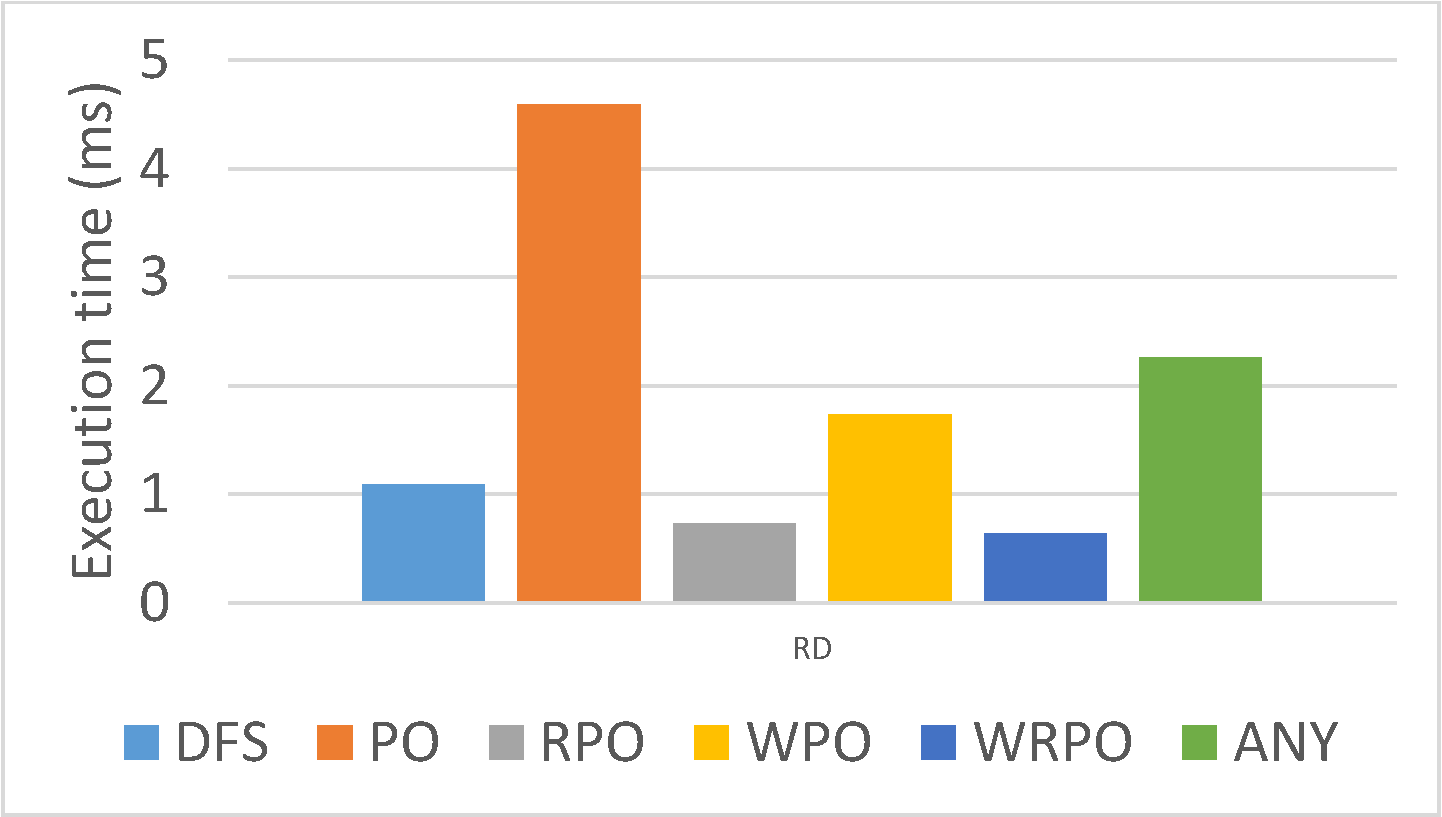
\includegraphics[width=.5\linewidth]{figures/motivation-a-rd}
}
\subfloat[Post-dominator analysis.] {
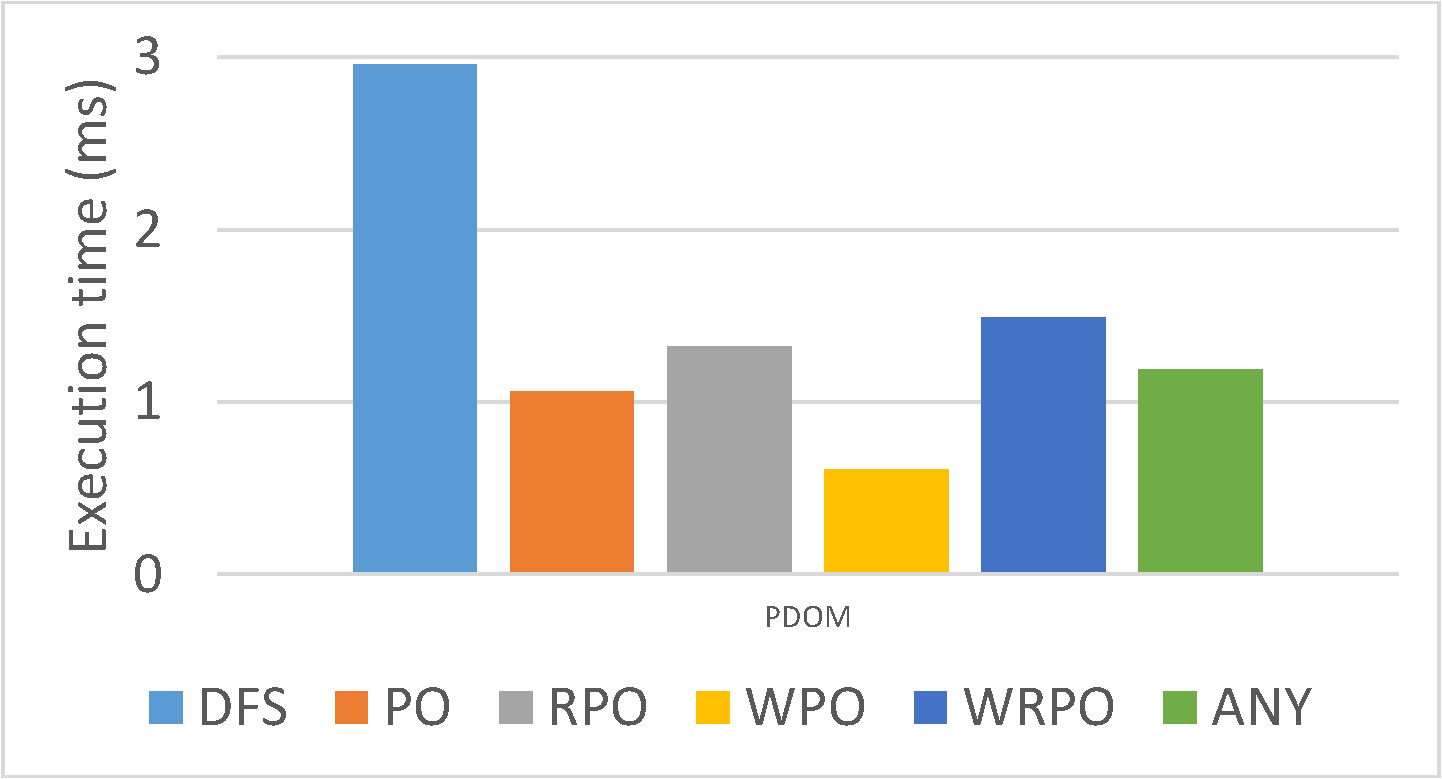
\includegraphics[width=.5\linewidth]{figures/motivation-a-pdom}
}\\
\subfloat[Collector analysis.] {
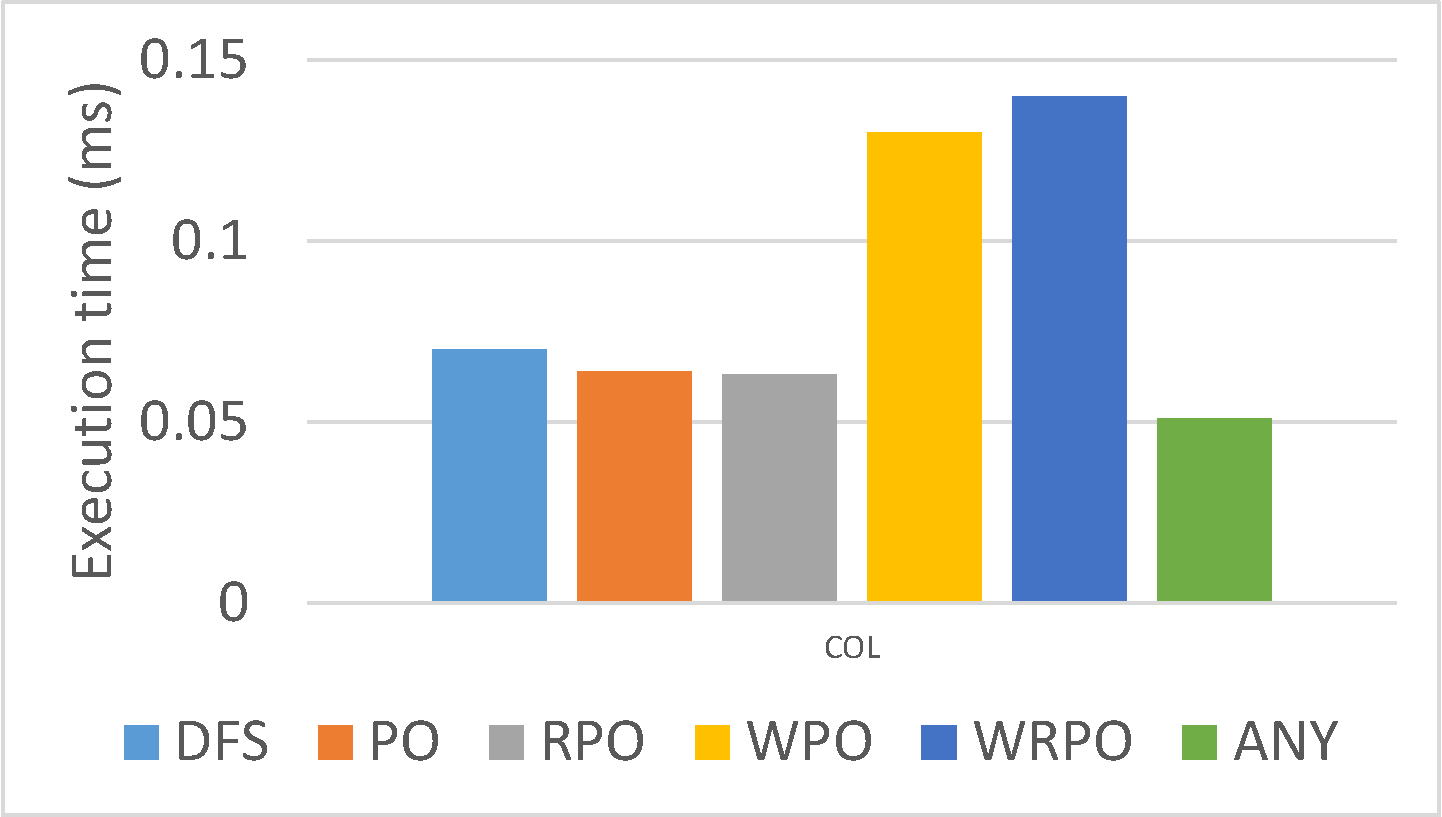
\includegraphics[width=.5\linewidth]{figures/motivation-a-col}
}
\caption{Running times (ms) of the three analyses on graph A using different traversal strategies.}
\label{fig:example-a-graph}
\end{figure*}

{\bf Motivation and Key Observations.\ }
To motivate, consider a software engineering task that infers the temporal 
specifications between pairs of API method calls, i.e., a call to $a$ must be 
followed by a call to $b$ by ~\cite{engler-sosp2001,ramanathan-icse2007,weimer-tacas2005,yang-icse2006}. 
A data-driven approach for inference is to look for pairs of API calls that frequently go in pairs in 
the same order at API call sites in the client methods' code. Such an 
approach contains (at least) three source code analyses on the control flow graph 
(CFG) of each client method: 
%
1) identifying references of the API classes and call sites of the API 
methods which can be done using \emph{reaching definition} analysis(~\cite{programanalysis}); 
%
2) identifying the pairs of API calls ($a$, $b$) where $b$ follows $a$ in the 
client code which can be done using \emph{post-dominator} analysis(~\cite{compilers}); and 
%
3) collecting pairs of temporal API calls by traversing all nodes in the 
CFG--let us call this \emph{collector} analysis. 
%
These analyses need to be run on a large number of client methods to 
produce temporal specifications with high confidence.

Implementing each of these analyses involves traversing the CFG 
of each client method. The traversal strategy could be chosen from a 
set of standard strategies e.g depth-first search (DFS), post-order 
(PO), reverse post-order (RPO), worklist with post-ordering (WPO), 
worklist with reverse post-ordering (WRPO) and any order (ANY).
In ANY order traversal strategy, nodes can
be visited in any order. In post-order traversal, the successors of
any node are visited before visiting the node, while in reverse post-order traversal, the
predecessors of any node are visited before visiting the node. In Worklist with Post-Order and Worklist with reverse post-order, the nodes are visited in the order they appear in the worklist. A worklist is a
data structure used to keep track of nodes to be visited. In WPO, worklist is
initialized with post-ordering of nodes, while in WRPO, The
worklist is initialized with nodes in the reverse post-order.

Figure \ref{fig:example-a-graph} shows the performance of each of these three 
analyses when using standard traversal strategies.
These runs are analyzing the CFG of a method in the DaCapo 
benchmark(~\cite{blackburn2006dacapo}). 
Actual implementation of this method is not important, but it suffices
to know that the CFG, which we shall refer to as Graph A, has 50 nodes
and has branches but no loops. Figure \ref{fig:example-a-graph} shows
that, for graph A, the WRPO performs better than other strategies for
the reaching definition analysis while the WPO outperforms the others
for the post-dominator analysis and the ANY traversal works best for
the collector analysis.

{\bf No Traversal Strategy Fits All.\ } The performance results are
somewhat expected, but require understanding the subtleties of the
analyses. Reaching definition analysis is a forward data-flow analysis
where the output at each node in the graph is dependent on the outputs
of their predecessor nodes.
So, DFS, RPO and WRPO by nature are the most suitable.
However, worklist is the most efficient strategy here because it
visits only the nodes that are yet to reach fixpoint unlike other
strategies that also visit notes that have already reached fixpoint.
Post-dominator analysis, on the other hand, is a backward analysis
meaning that the output at each node in the graph is dependent on the
outputs of their successor nodes. Therefore, the worklist with
post-ordering is the most efficient traversal.
For the collector analysis, any order traversal works better than
other traversal strategies for graph A. This is because for this
analysis the output at each node is not dependent on the output of any
other nodes and hence it is independent of the order of nodes visited.
The any order traversal strategy does not have the overhead of
visiting the nodes in any particular order like DFS, PO, RPO nor the
overhead to maintain the worklist. Therefore any order traversal
performs better than other traversal strategies.

{\bf Properties of Input Graph Determine Strategy.\ }
For the illustrative example discussed above, DFS and RPO were worse
than WRPO for the reaching definition analysis and PO was worse than
WPO for post-dominator because they require one extra iteration of
analysis to be performed and realize that fixpoint has been reached.
However, since graph A does not have any loops, if the graph A's nodes
are visited in such a way that each node is visited after its
predecessors for reaching definition analysis and after its successors
for post-dominator analysis, then the additional iteration is actually
redundant. Given that graph A has no loops, one could optimize RPS or
PO to bypass the extra iteration and fixpoint checking. Thus, the
optimized RPS or PO would run the same number of iterations as the
respective worklist-based ones and finish faster than them because the
overhead of maintaining the list is eliminated.

\begin{figure}
\centering
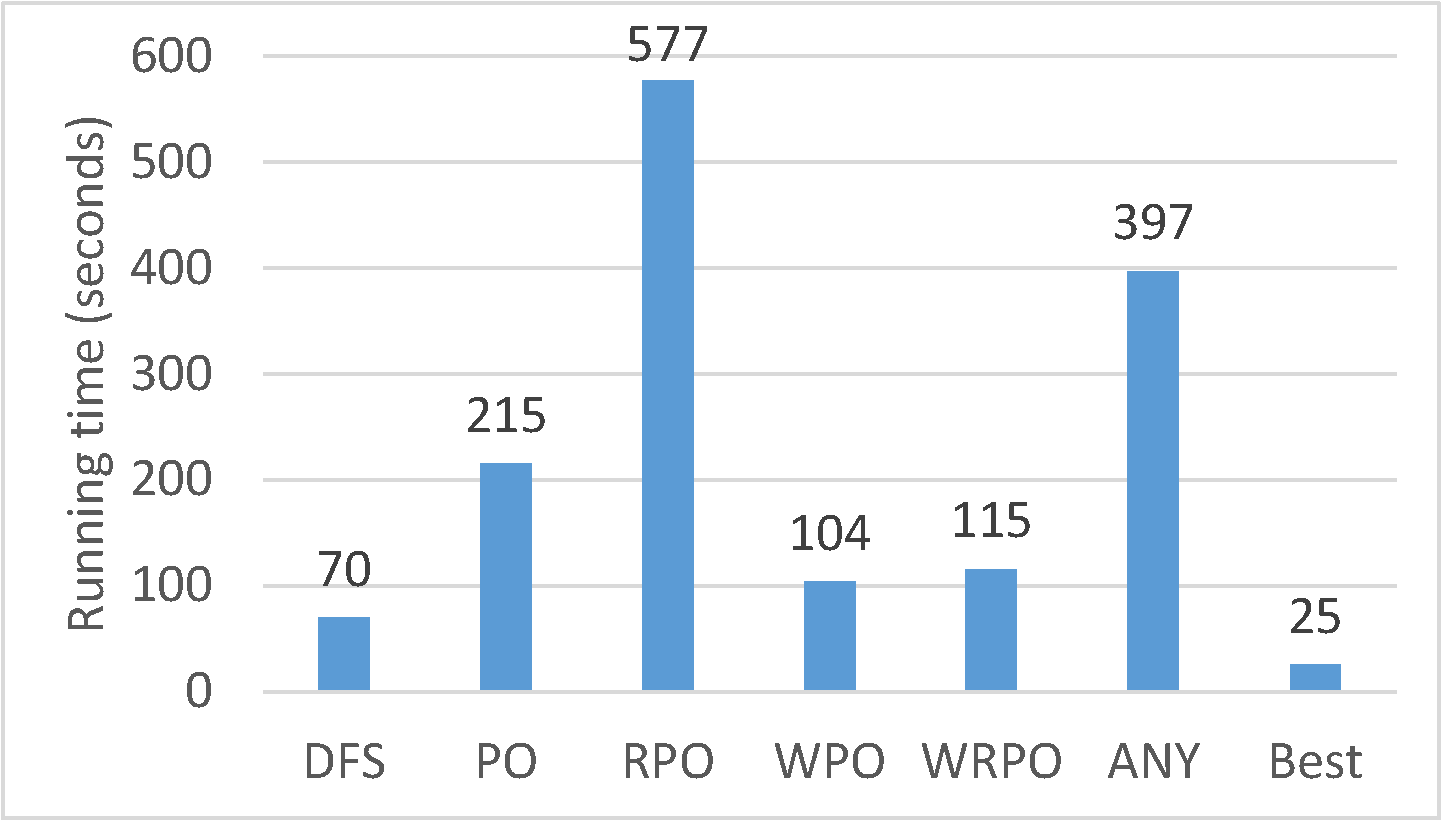
\includegraphics[width=.6\textwidth]{figures/motivation-sum.pdf}
\caption{Running times of three analyses using different traversal strategies on a large codebase.}
\label{fig:motive}
\end{figure}

The potential gains of selecting a suitable traversal strategy can be 
significant.
To illustrate, consider \figref{fig:motive} that shows the performance of 
our entire illustrative example (inferring temporal specifications) on a 
large corpus of 287,000 CFGs extracted from the DaCapo
benchmark dataset(~\cite{blackburn2006dacapo}).
\figref{fig:motive} shows the 
bar chart for the total running times of the three analyses. The \textbf{Best}
 strategy is an ideal one where we can always choose the most efficient with 
all necessary optimizations. The bar chart confirms that fixing a traversal 
strategies for running different analyses on different types of graphs is not 
efficient. Selecting and optimizing traversal strategy for each analysis on 
each graph is desirable. Such a strategy could reduce the running time on a 
large dataset from 64\% (against DFS) to 96\% (against RPO).

Our approach relies on our observations that a suitable traversal strategy is
dependent on both the source code analyses and input graphs' properties.
The former are static properties and the latter are runtime properties.
More importantly, depending on the properties of analyses and graphs, existing
traversals could be optimized to improve their performance.  
We have evaluated our technique using a set of 21 source code analysis that
includes control and data-flow analysis, and analysis to find bugs. The
evaluation is performed on two datasets: a dataset containing well-maintained
projects from DaCapo benchmark (contains a total of 287K graphs), and a
ultra-large dataset containing more than 380K projects from GitHub (contains a
total of 162M graphs). Our evaluation shows that our technique successfully selected
the most time-efficient traversal strategy for 99.99\%--100\% of the time and
using the selected traversal strategy and optimizing it, the running times of a
representative collection of source code analysis in our evaluation
were considerably reduced by 1\%-28\% (13 minutes to 72 minutes in absolute time) when compared against the best performing traversal strategy.
The overhead imposed by our approach is negligible (less than 0.2\% of the total 
running time for a large dataset and less than 0.01\% for an ultra-large dataset). 

The rest of the thesis is organized as follows. Chapter 2 lists the contribution of our work. Chapter 3 gives a background of many ideas that this thesis builds upon, such as Graph and its traversal, various traversal strategies, Program analysis, Control and data flow analysis. Chapter 4.1 describes our system For expressing source code analysis as traversals, while Chapter 4.2 presents the factors that influence the selection of the optimal traversal strategy for any given traversal. Chapter 4.3 lists all the candidate traversal strategies while Chapter 4.4 describes our decision tree to select traversal strategy and also presents an example analysis and graph and walks through the decision tree. Chapter 5 gives the implementation detail on how we extended Boa language to have hybrid capability. Chapter 6 presents our experimental setup and the dataset used. Chapter 7 provides the evaluation and the anlaysis that we did on running time comparison between hybrid and various other strategies. Chapter 8 presents the correctness of analysis using Hybrid approach. Chapter 9 presents the Hybrid's traversal strategy prediction precision. Chapter 10 analyses our decision tree's distribution while Chapter 11 analyses the importance of our traversal optimization. Chapter 12 discusses the two case studies that we implemented using our formalism for source code analysis and their results. Chapter 13 discusses about the threat to validity while Chapter 14 discusses related work. Chapter 15 concludes and gives some possible ideas for future work.
\chapter{Contributions}

In this work, we develop {\em hybrid traversal selection}, a novel program
analysis optimization technique for BigCode analyses expressed as graph traversals.
Our approach relies on our observations that a suitable traversal strategy is
dependent on both the program analyses and input graphs' properties.
The former are static properties and the latter are dynamic properties.
More importantly, depending on the properties of analyses and graphs, existing
traversals could be optimized to improve their performance.  
Hybrid traversal selection relies on several technical underpinnings: 

\noindent{\bf [Traversal Declaration and Traverse Expression]} 
Programmers can declare their program analyses
as one or more {\bf traversal} declarations and run them using {\bf traverse} expression.
The runtime implementation of the {\bf traverse} expression selects a suitable 
traversal strategy based on the {\bf traversal} declaration and the input graph.
Main benefit of these linguistic abstractions is that they abstract away 
traversal related code so that the traversal strategy can be replaced as needed 
by the analysis runtime.

\noindent{\bf [Data-Flow and Loop Sensitivity Analyses for Traversals]}
We show that traversal strategy selection depends on three critical properties
of the traversal: {\em data-flow sensitivity}, {\em loop sensitivity}, and 
{\em traversal direction}. We propose algorithms for computing these properties.
Our analysis system implements these algorithms.
These properties are computed statically and their values are stored as metadata 
to be utilized by the traversal selection at runtime.

\noindent{\bf [Graph \Graphprop{}]}
We have observed that the traversal strategy selection depends on one
dynamic property of the input which is {\em graph \graphprop{}}. This property partitions
the set of graphs into three categories: those that are sequential, those with branches
but no cycles, and those with cycles. Our system computes this property at 
graph construction time and stores it as an attribute in the runtime graph representation. 

\noindent{\bf [Decision Tree for Traversal Strategy Selection]}
We have devised a {\em decision tree} for traversal strategy selection that 
given data-flow sensitivity, loop sensitivity, and traversal direction properties 
of the analysis and the \graphprop{} property of the input graph produces 
a selection for traversal strategy.
While the tree is utilized by our automated system, it could also be used by 
a programmer for manual traversal selection.

Hybrid traversal selection has two direct benefits. First, it improves the 
efficiency of BigCode analysis thus speeding up data-driven science in this important area.
Second, it frees up programmers from having to write traversal related code 
and then optimizing it based on the analysis and the graph at hand. 

We have evaluated our technique using a set of 21 source code analysis that
includes control and data-flow analysis, and analysis to find bugs. The
evaluation is performed on two datasets: a dataset containing well-maintained
projects from DaCapo benchmark (contains a total of 287K graphs), and a
ultra-large dataset containing more than 380K projects from GitHub (contains a
total of 162M graphs). Our evaluation shows that our technique successfully selected
the most time-efficient traversal strategy for 99.99\%--100\% of the time and
using the selected traversal strategy and optimizing it, the running times of a
representative collection of source code analysis in our evaluation
were considerably reduced by 1\%-28\% (13 minutes to 72 minutes in absolute time) when compared against the best performing traversal strategy. The case studies show that hybrid traversal reduces 80--175 minutes in running times for three software engineering tasks.
The overhead imposed by our approach is negligible (less than 0.2\% of the total 
running time for a large dataset and less than 0.01\% for an ultra-large dataset). 

In summary, this paper makes the following contributions:
\begin{itemize}
	\item It describes a system for expressing source code analysis as traversals. The
	constructs and operations in the system allows different source code analysis to
	be expressed in a manner that allows automatic selection of the best traversal
	strategies.
	\item It defines a set of novel properties about the traversal expressed 
	in our system. It also describes algorithms for analysing traversals for inferring 
	these properties. 
	\item It describes a novel decision tree for selecting the most suitable traversal 
	strategy. The static and runtime properties also allows
	certain optimizations to be performed on the selected traversal strategy to
	further improve the performance.
	\item It demonstrates the potentially broad range of applications of
	hybrid traversal selection for optimizing source code analysis such
	as available expressions, local may alias, live variable, nullness
	analysis, post dominator, reaching definitions, resource status,
	very busy expression, etc.
\end{itemize} 

% The rest of the paper is organized as follows: the next section
% (\secnref{sec:language}) describes our system for expressing program analysis as
% traversals, followed by an overview of our approach in \secnref{sec:overview}.
% Key details about our hybrid technique is provided in \secnref{sec:approach}.
% Section \secnref{sec:eval} presents our evaluation, followed by a discussion of
% the key related works in \secnref{sec:related} and a conclusion.
% 
% 
% The next section describes the constructs that we are going to use describe
% our analysis. This construct will in-turn be used in our algorithms to
% analyze our analysis.

% 
% Graph traversal is a well-studied problem, and various traversal strategies
% exist e.g. the postorder, reverse postorder, worklist-based traversal, etc.
% These strategies significantly outperform the alternative when applied to the
% kind of program artifacts that suits them well.
% On the other hand, adopting a traversal that is not suitable to the artifact may
% lead to more traversals over the graphs and more operations per node for the
% analysis. \newline
% 
% Software repositories like  SourceForge (350,000+ projects), GitHub (250,000+
% projects), and Google Code (250,000+ projects) contain massive codebases, also
% called Big code.
% Big code mining as its most basic operation contains huge number of traversals
% of the AST and other derived artifacts such as the control flow graph (CFG), the
% data-flow graph (DFG), etc. These artifacts are of different kinds. So,
% selecting a single traversal strategy may not be desirable. And the mining task
% that needs to be performed on such large scale data can have various
% characteristics that they may warrant a particular strategy. Selecting a
% in-appropriate traversal may lead to significant increase in execution time and
% for such large scale software repository
% analysis~\cite{bajracharya2014sourcerer},
% ~\cite{bevan2005facilitating},~\cite{gousios2009alitheia},~\cite{gousios2012ghtorrent}
% this could be costly.\newline
% 
% Our hybrid approach is based on the intuition that the analysis task that needs
% to be performed can have different characteristics and the large scale data that
% the analysis has to be performed upon contains artifacts of different
% characteristics. These information may lead us to the traversal strategy best
% suited for the analysis and the artifact. Leveraging this information from
% analysis code statically and information from artifact dynamically, we can apply
% the best traversal that needs fewer node visits and fewer operations per node to
% perform the analysis when compared to other approaches.\newline
% 
% We have applied our approach to twenty traversal-based formulation of fairly
% standard program analyses, showing broad applicability of our ideas. For these
% analyses we see an improvement between 10-40\% over existing traversal
% strategies in terms of the total execution time. Most importantly, hybrid
% approach improves performance significantly from worklist approach which is the
% most used approach for solving data flow analysis. We achieve these performance
% gain without compromising the soundness of the result. Last but not least, we
% show very high accuracy in traversal selection between 99-100\% owing to our
% selection criteria and algorithms. We believe that our approach can help
% decrease the turnaround time of data-driven experiments in this area.
% 
% We summarize the other contribution of this paper to realize hybrid traversal
% selection:
% \begin{itemize}
% 	\item Proposed efficient way of identifying the static properties(data flow sensitivity, loop sensitivity) from the analysis code.
% 	\item A decision tree to identify the best traversal strategies among the candidates based on the static properties of the traversal and the dynamic property of the graph.
% 	\item Identified the optimization that could be performed on the selected traversal strategy that makes it the traversal that has the best execution time among the candidates for the given analysis and the graph.
% 	\item Introduced a traversal property called "Loop sensitivity" for data flow analysis that identifies whether the loops present in the graph introduces more traversal of the graph to reach fixpoint.
% 	%\item Identified the characteristics of the analysis and the input graph for which fix point checking is redundant for data flow analysis.
% 	%\item Proposed efficient way of identifying the dynamic properties(type of control flow) from the CFG.
% \end{itemize}

\chapter{Hybrid Traversal Selection for Efficient Source Code Analysis}
\label{sec:approach}
\label{sec:overview}
 
In this chapter we first provide a brief overview of our technique, 
followed by an overview of the constructs used for expressing source code analyses.
We then describe properties, analyses, and a decision tree that are 
the technical underpinnings of our selection technique.

\begin{figure*}[ht!]
  \centering 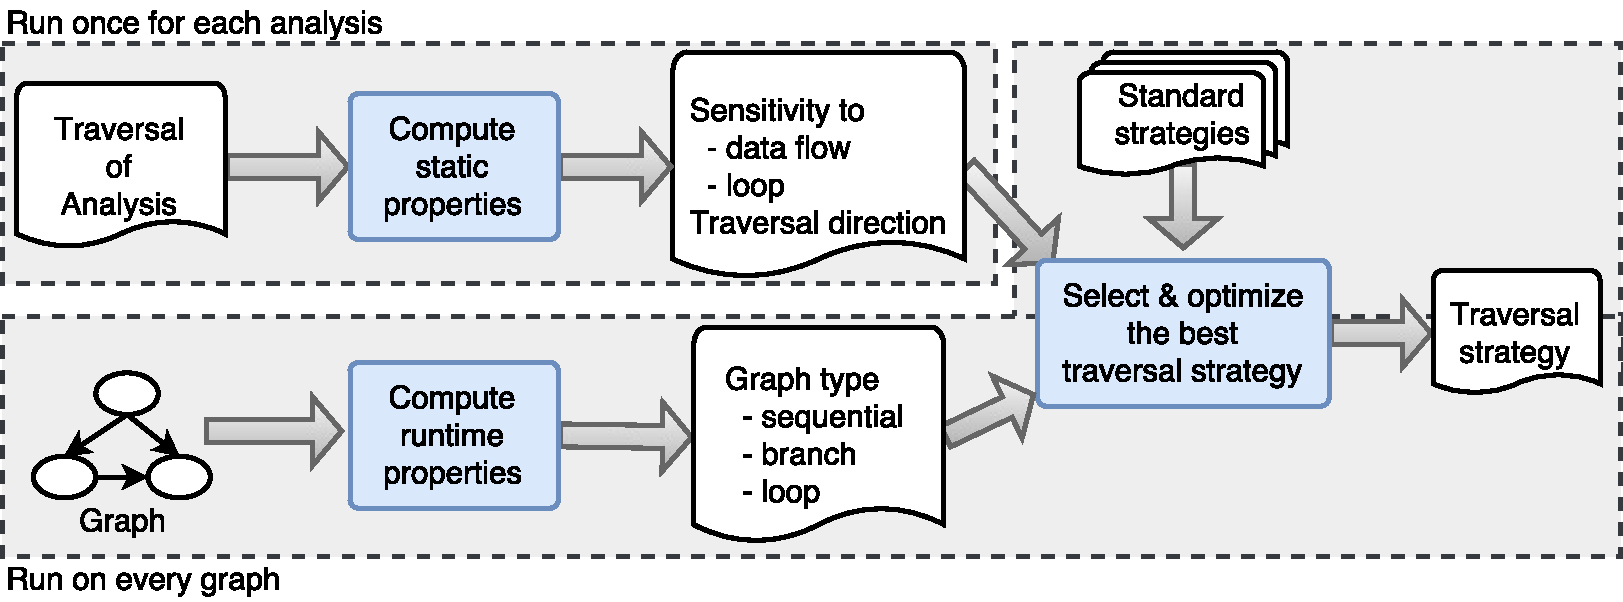
\includegraphics[width=0.9\linewidth]{figures/hybrid-overview.pdf}
\caption{Overview of the hybrid approach for selecting and optimizing graph traversal strategy.}
  \label{fig:overview}
\end{figure*}

\fignref{fig:overview} provides an overview of our approach and its key components.
Inputs to our approach are source code analysis that contains one or more 
traversals (\secref{sec:language}), and a graph. 
Output of our technique is an optimal traversal strategy for every
traversal in the analysis. For selecting an optimal traversal strategy for a
traversal, our technique computes a set of static properties of 
the analysis (\secref{sec:compute-properties}),
such as data-flow sensitivity, loop sensitivity, and extracts a runtime property
about the graph that defines the \graphprop{} in the graph
(sequential/branch/loop). Upon computing the static and runtime properties, our
approach selects a traversal strategy from a set of candidate strategies (\secref{sec:candidates}) for
each traversal in the analysis (\secref{sec:decision-tree}) and 
optimizes it (\secref{subsec:optimizations}). The static properties of the
traversals are computed only once for each analysis, whereas graph \graphprop{} 
is determined for every input graph.

\section{A System For Expressing Source Code Analysis As Traversals}
\label{sec:language}
% \section{Program analysis and traversals}
% \label{sec:programanalysis}
A source code analysis is performed on various source code artifacts such as
source code text, intermediate representations like abstract syntax trees
(ASTs), graph-based representations like control flow graphs (CFGs) and call
graphs (CGs), etc. In our system, source code analysis such as control- and
data-flow analysis are expressed as traversals over CFGs.

\begin{definition}\label{def:cfg}
A control flow graph (CFG) is a directed graph $G$ = $(N, E, n_{start},
N_{end})$ with a set of nodes $N$ representing the program statements and a set
of edges $ E \subseteq N \times N$ representing the control flow relation
between the program statements. A CFG has a single start node, $n_{start}$, and
a set of end nodes, $N_{end}$.
\end{definition}

% A source code analysis such as control flow analysis, data-flow analysis, etc can be
% expressed as traversals over program graphs.
% \begin{definition}\label{def:cfg}
% A \textbf{Program Graph} of a program is defined as $G$ = $(N, E, n_{start},
% N_{end})$, where $G$ is a directed graph with a set of nodes $N$ representing program statements,
% and a set of edges $ E \subseteq N \times N$ representing analysis relevant
% relationship between the nodes in the graph.
% 
% representing possible flow of execution between the nodes in the
% graph.
% A program graph has a single start, $n_{start}$, and a set of end nodes, 
% $N_{end}$.
% All the nodes in a program graph are reachable from the $n_{start}$ and the
% $n_{end}$ node is reachable from all nodes in the program graph.
% \end{definition}
For any node $n \in N$, $n.preds$ is a set of immediate predecessors, $n.succs$
is a set of immediate successors, $n.stmt$ provides the program statement at the
node, and $n.id$ is a unique identifier of the node. Here on, we use graph to
refer to CFG.
% Note that, depending on the analysis, node ids are assigned while constructing
% the graph. For instance, in case of control flow graphs, node ids may be
% assigned in the order of the flow of execution.
% Note that, node ids are assigned in the order of the flow of
% execution, while constructing a graph. 
% Examples of program graph includes control flow graph (CFG), control dependence
% graph (CDG), program dependence graph (PDG), etc. Hereon, we refer to program
% graphs simply as graphs. 
% 
% \newline \tab $n.preds = P$ where $P =
% \{p_{0}, p_{1},.., p_{p}\}$ such that $\forall p_{i}, (p_{i}, n) \in E$,
% \newline \tab $n.succs = S$ where $S = \{s_{0}, s_{1},.., s_{s}\}$ such that
% $\forall s_{i}, (n, s_{i}) \in E$, \newline \tab $n.stmt$ = program statement
% contained in the node $n$, \newline \tab $n.id$ = unique identifier of the node
% $n$. $ids$ are integers that are assigned to the nodes in topological order.
% \end{definition}

A source code analysis over a graph visits nodes in the graph in certain order
and collects information at nodes (aka, analysis facts or outputs). For
instance, the {\em reaching definition} analysis over a CFG, visits every node
in the CFG and collects the variable definitions at nodes as analysis facts.
An analysis may require multiple traversals over a graph and each traversal may
visit nodes multiple times (for fixpoint).
For instance, the {\em reaching definition} analysis requires two traversal of
the CFG: an {\em initialization} traversal for collecting the variable
definitions at nodes as analysis facts, and a {\em propagation} traversal for
propagating the analysis facts along the graph. The {\em initialization}
traversal visits every node exactly once, whereas the {\em propagation}
traversal may visit the nodes multiple times until a fixpoint is reached and the
analysis facts at nodes does not change further.

% A program analysis, such as control or data flow analysis visits nodes in
% the CFG, in certain order, and collects analysis facts at nodes. For
% instance, the {\em reaching definition} analysis visits every node in the CFG
% and collects variable definitions at nodes as analysis facts. An analysis
% may require multiple traversals of a CFG. For instance, the {\em reaching
% definition} analysis, in the {\em initialization} traversal, collects variable
% definitions at nodes as analysis facts, and in the {\em propagation}
% traversal, updates the analysis facts until a fixpoint is reached, where no
% further changes to analysis facts at nodes is required.

In our system, a source code analysis over a graph is expressed by defining and
invoking one or more traversals. A traversal is defined using a special
\lstinline|traversal| block: 
\begin{lstlisting} 
t := traversal(n : Node) : T { tbody }
\end{lstlisting}
In this traversal block definition, \lstinline|t| is the name of the traversal
that takes a single parameter \lstinline|n| representing the graph node that is
being visited. A traversal may define a return type \lstinline|T| representing
the output type. The output type can be a primitive or a collection data type. A
block of code that generates the traversal output at a graph node is given by
\lstinline|tbody|. The \lstinline|tbody| may contain common statements and
expressions, such as variable declarations, assignments, conditional statements,
loop statements, and method calls, along with some special expressions discussed
in this chapter.
% 
% 
% A traversal visits every node in the control flow graph and executes a block of
% code. The traversal visits the nodes in a certain fashion and produces a output
% of certain type for each node. Signature to express our traversals is shown
% below.
%\begin{verbatim}
	%t := traversal(n : Node) : OType { tbody }
%\end{verbatim}
% 
% The traversal block shown above defines a variable \lstinline|t| of
% traversal type and the traversal visits every node in the graph in certain order
% and while visiting a node \lstinline|n|, it executes a block of code
% \lstinline|tbody| to produce an output of type \lstinline|T| for the
% visited node.
% 
% A \lstinline|traversal| block always take one parameter of type \lstinline|Node|
% representing a graph node, and it has an optional output type,
% \lstinline|T|.
% The output type can be a primitive or a collection data type. 
% Semantically, a traversal that defines \lstinline|T|, generates and collects
% analysis facts for nodes in the graph.
% A block of code that generates the analysis facts at a graph node is given by
% \lstinline|tbody|. The instructions or operations in the \lstinline|tbody| block
% is defined in the language for expressing the source code analysis. A traversal
% block can be assigned a name, \lstinline|t| in the above listing, which
% can be used to invoke the traversal. The type of \lstinline|t| is a
% special traversal type. 

A traversal can be invoked using a special \lstinline|traverse| expression:
\begin{lstlisting}
traverse(g, t, d, df, ls, fp)
\end{lstlisting}

A \lstinline|traverse| expression takes six parameters: \lstinline|g| is the
graph to be traversed, \lstinline|t| is the traversal to be invoked,
\lstinline|d| is the traversal direction and \lstinline|df|, \lstinline|ls|, \lstinline|fp| are optional
parameters. \lstinline|df| is of boolean type which indicates whether the analysis is data flow sensitive or not. \lstinline|ls| is also an boolean variable, indicating whether the analysis is loop sensitive or not. If \lstinline|df| is not provided, Algorithm 1 in Chapter 3.2.1 will be used to compute this property. Similarly, if \lstinline|ls| is not provided, Algorithm 2 in Chapter 3.2.3 will be used to compute this property. \lstinline|fp| is a variable name of the user defined fixpoint function. A
traversal direction is a value from the set \{\lstinline|FORWARD|,
\lstinline|BACKWARD|, \lstinline|ITERATIVE|\}, where \lstinline|FORWARD| is used
to represent a forward analysis (predecessors of a node are processed before the
node), \lstinline|BACKWARD| is used to represent a backward analysis (successors
of a node are processed before the node), and \lstinline|ITERATIVE| is used to
represent a sequential analysis (visits nodes as they appear in the nodes
collection).
A user defined fixpoint function can be defined using the \lstinline|fixp|
block:
\begin{lstlisting}
fp := fixp(...) : bool { fbody }
\end{lstlisting}

In this \lstinline|fixp| block, \lstinline|fixp| is a keyword for defining a
fixpoint function. A fixpoint function can take any number of parameters, and it
must always return a boolean. The body of the fixpoint function is defined in
the \lstinline|fbody| block. A fixpoint function can be assigned a name, which
can be passed in the \lstinline|traverse| expression.

\para{Accessing Facts of Other Nodes}
We also provide a special expression \lstinline|output(n, t)| for querying the
traversal output associated with a graph node \lstinline|n|, in the traversal
\lstinline|t|.

\begin{table*}[ht!] \centering \small
\caption{Syntax reference.}
\label{tab:syntax}
% \resizebox{\textwidth}{!}{
\begin{tabular}{|p{1.5cm}|p{2.5cm}|p{11cm}|}
\hline 
\textbf{Construct} & \textbf{Syntax} & \textbf{Description}\\\hline
Traversal & \lstinline|t := traversal(n : Node) : T { tbody }| & \lstinline|t| is the name of the traversal that takes a single parameter \lstinline|n| representing the graph node that is being visited. A traversal may define a return type \lstinline|T| representing the output type. A block of code that generates the traversal output at a graph node is given by \lstinline|tbody|.\\\hline
Traverse & \lstinline|traverse(g, t, d, df, ls, fp)| & \lstinline|g| is the
graph to be traversed, \lstinline|t| is the traversal to be invoked,
\lstinline|d| is the traversal direction and \lstinline|df|, \lstinline|ls|, \lstinline|fp| are optional
parameters. \lstinline|df| is of boolean type which indicates whether the analysis is data flow sensitive or not. \lstinline|ls| is also an boolean variable, indicating whether the analysis is loop sensitive or not. \lstinline|fp| is a variable name of the user defined fixpoint function. A traversal direction is a value from the set \{\lstinline|FORWARD|,
\lstinline|BACKWARD|, \lstinline|ITERATIVE|\}\\\hline 
Fixpoint & \lstinline|fp := fixp(...) : bool { fbody }| & \lstinline|fixp| is a keyword for defining a fixpoint function. A fixpoint function can take any number of parameters, and it
must always return a boolean. The body of the fixpoint function is defined in
the \lstinline|fbody| block.\\\hline 
Output & \lstinline|output(n, t)| & \lstinline|output| is used for querying the
traversal output associated with a graph node \lstinline|n|, in the traversal
\lstinline|t|\\\hline 
\end{tabular}
% }
\end{table*}

% 
% 
% 
% \lstinline|tbody| represents the block of code that will be executed when
% traversing a node. Here \texttt{t} is the name of the traversal.
% The traversal \texttt{t} produces a output of OType for each visited node. This
% output can be queried by a special function \textit{output} which takes the form
% given below.
% \begin{verbatim}
% 			output(n, t)
% \end{verbatim}
% Here \texttt{n} represents the node and \texttt{t} represents the traversal.
% \textit{output} returns the output associated with the node n visited in the
% traversal t. In-order to invoke a traversal on a control flow graph, we use the
% \textit{traverse} operation.
% \begin{verbatim}
% 			traverse(g, t, d, fp); 
% \end{verbatim}
% The \textit{traverse} operation takes four arguments. where \texttt{g} is the
% control flow graph to be traversed, \texttt{t} is the traversal, \texttt{d} is
% the traversal direction which can take either of the two values
% \{\texttt{FORWARD}, \texttt{BACKWARD}\}, \texttt{fp} is the optional user
% defined fixpoint function, which will run the traversal until the fixpoint
% condition is satisified by all the nodes. Fixpoint function has the following
% syntax.
% \begin{lstlisting}[caption={Fixpoint construct.},label={lst:fixp}]
% fp := fixp(...) : bool {
%         fbody
% }
% \end{lstlisting}
% Here \textit{fixp} is a keyword and it can take any number of parameters and
% always returns a boolean. \texttt{fp} is the name of the fixpoint fucntion and
% \texttt{fbody} is the user written block of code. If the return value is
% \texttt{TRUE}, then it indicates that the fixpoint is reached. \newline There is
% no option to specify the traversal strategy in traverse operation as the best
% traversal strategy will be decided based on the input control flow graph and the
% body of the traversal. \newline

\begin{table*}[ht!] \centering \small
\caption{Operations on collections.}
\label{tab:operations}
% \resizebox{\textwidth}{!}{
\begin{tabular}{|l|l|}
\hline 
\textbf{Operation} & \textbf{Description}\\\hline
\lstinline|add(C, e)| & Adding an element e to collection C \\\hline
\lstinline|addAll(C1, C2)| & Adding all elements from collection C2 to collection
C1\\\hline 
\lstinline|remove(C, e)| & Removing an element e from collection C \\\hline 
\lstinline|removeAll(C1, C2)| & Removing all elements from collection C1 that are
also present in collection C2\\\hline 
\lstinline|get(C, i)| & Element at index i from collection C is accessed\\\hline
\lstinline|has(C, e)| & Checking if collection C has element e\\\hline
\lstinline|equals(C1, C2)| & Checking if collection C1 and collection C2 has the
same elements\\\hline 
\lstinline|C1 = C2| & Assigning collection C2 to collection C1\\\hline
\lstinline|union(C1, C2)| & Returns the union of the elements in collection C1 and
collection C2\\\hline 
\lstinline|intersection(C1, C2)| & Returns the intersection of the elements in collection C1 and collection C2\\\hline
\end{tabular}
% }
\end{table*}
\para{Data Types and Collections}
% \label{sec:Data-Types}
Our system for expressing source code analysis as traversals provides primitive and
collection data types. Primitive types include: \lstinline|bool, int, string|
and collection types include: \lstinline|Set and Seq|, where \lstinline|Set| is a
collection with distinct and unordered elements, whereas, \lstinline|Seq| is a
collection with distinct and ordered elements. A set of operations that can be
performed on collection types is described in \tabref{tab:operations}.
% 
% There are three primitive types (bool , int , string) that could be used in our
% traversal. We also provides two types of collection : Set and Sequence. Elements
% in a Set are unique but unordered. Elements in a Sequence are not unique but
% ordered. Operations that are allowed in the collection are specified in Table
% \ref{tab:operations}.

To summarize, we described a system for expressing source code analysis as
traversals over graphs using two special constructs: \lstinline|traversal| for
defining a traversal, and \lstinline|traverse| for invoking a defined traversal. 
A traversal may visit graph nodes multiple times (in case of fixpoint) and it
can be invoked using several parameters specifying the direction of the
traversal, a user defined fixpoint function, etc.
A traversal output associated with graph nodes can be queried using a special
expression \lstinline|output()|. 
To be able to express a variety of source code analysis, our system provides
primitive and collection datatypes with well-defined operations.
Later in this chapter we demonstrate how the constructs and operations of the
system enables determining properties of the source code analysis expressed
in our system, such that optimal traversal strategies can be automatically
selected.

% We also provide a special expression \lstinline|output()| to query the analysis
% output of nodes and a set of operations to compose and manipulate traversal
% output of nodes. 
% The special constructs and operations defined here solves a
% challenging problem of determining certain static properties of the analyses, as
% described in \secnref{sec:compute-properties}.
\para{An Example: Post dominator analysis} We now describe how to use our system
to express source code analysis as traversals using an example source code analysis.
Post dominator analysis is a backward control flow analysis that collects node
ids of all nodes that post dominates every node in the CFG~\cite{compilers}.
This analysis can be expressed using our system as shown in Listing
\ref{lst:dominators}.

\begin{lstlisting}[basicstyle=\footnotesize\ttfamily, numbers=left, numbersep=-8pt, 
escapechar=@, caption={Post dominator analysis: an example source code analysis
expressed using our system.}, label={lst:dominators}] 
	allNodes: Set<int>;
	initT := traversal(n: Node) { 
		add(allNodes, n.id);
	}
	domT := traversal(n: Node): Set<int> { 
		Set<int> dom;
		if (output(n, domT) != null) {
			dom = output(n, domT);
		} else {
			if (node.id == exitNodeId) {
				dom = {};
			} else {
				dom = allNodes;
			}
		}
		foreach (s : n.succs) 
			dom = intersection(dom, output(s, domT)) 
		add(dom, n.id); 
		return dom; 
	} 
	fp := fixp(Set<int> curr, Set<int> prev): bool {
		if(equals(curr, prev))
			return true;
		return false;
	}
	traverse(g, initT, ITERATIVE); @\label{line:traverse}@
	traverse(g, domT, BACKWARD, fp); 				
\end{lstlisting}

Listing \ref{lst:dominators} mainly defines two traversals \textbf{\lstinline|initT|}
(lines 2-4) and \textbf{\lstinline|domT|} (lines 5-20), and invokes them using
\textbf{\lstinline|traverse|} expressions (lines 26 and 27). Line 21-25 defines a
fixpoint function using \textbf{\lstinline|fixp|} block, which is used in the
\textbf{\lstinline|traverse|} expression in line 27. Line 1 defines a variable
\textbf{\lstinline|allNodes|} of collection type \textbf{\lstinline|Set|}, where
\textbf{\lstinline|Set<int>|} defines a collection type \textbf{\lstinline|Set|} with elements of
type \textbf{\lstinline|int|}. Line 3 uses an operation \textbf{\lstinline|add|} (defined in
\tabref{tab:operations}) on collection \textbf{\lstinline|allNodes|}. The common
statements and expressions used in the language to express the analysis are not
described in our system, however all standard statements and expressions are
allowed.
For instance, \textbf{\lstinline|if-else|} statements are used in lines 7-15,
\textbf{\lstinline|foreach|} iteration is used in lines 16-17, and so on.
Lines 26 and 27 provides two flavors of invoking traversals using
\textbf{\lstinline|traverse|} expressions: one without a fixpoint and other with a
user-defined fixpoint function. A usage of special expression
\textbf{\lstinline|output(n, domT)|} can be seen in line 8. The traversal
\textbf{\lstinline|initT|} does not define any output for CFG nodes, whereas, the
traversal \textbf{\lstinline|domT|} defines an output of type \textbf{\lstinline|Set<int>|} for
every node in the CFG. For managing the analysis output of nodes,
\textbf{\lstinline|domT|} traversal maintains an internal map that contains analysis
output for every node, which can be queried using \textbf{\lstinline|output(n, domT)|}.
A pre-defined variable \textbf{\lstinline|g|} that represents the CFG is used in the
\textbf{\lstinline|traverse|} expressions in lines 26 and 27.

\begin{figure}[ht!]
\centering
% \caption{}
% % 
% % 
% % Dominator analysis performs traversal over the graph to determine the
% % dominators of each node. It has two traversals. \textit{init} traversal collects
% % all node ids. \textit{dom\_T} is called with a fixpoint and it runs till all the
% % nodes reach the fixpoint condition.}
% \label{fig:dominator}
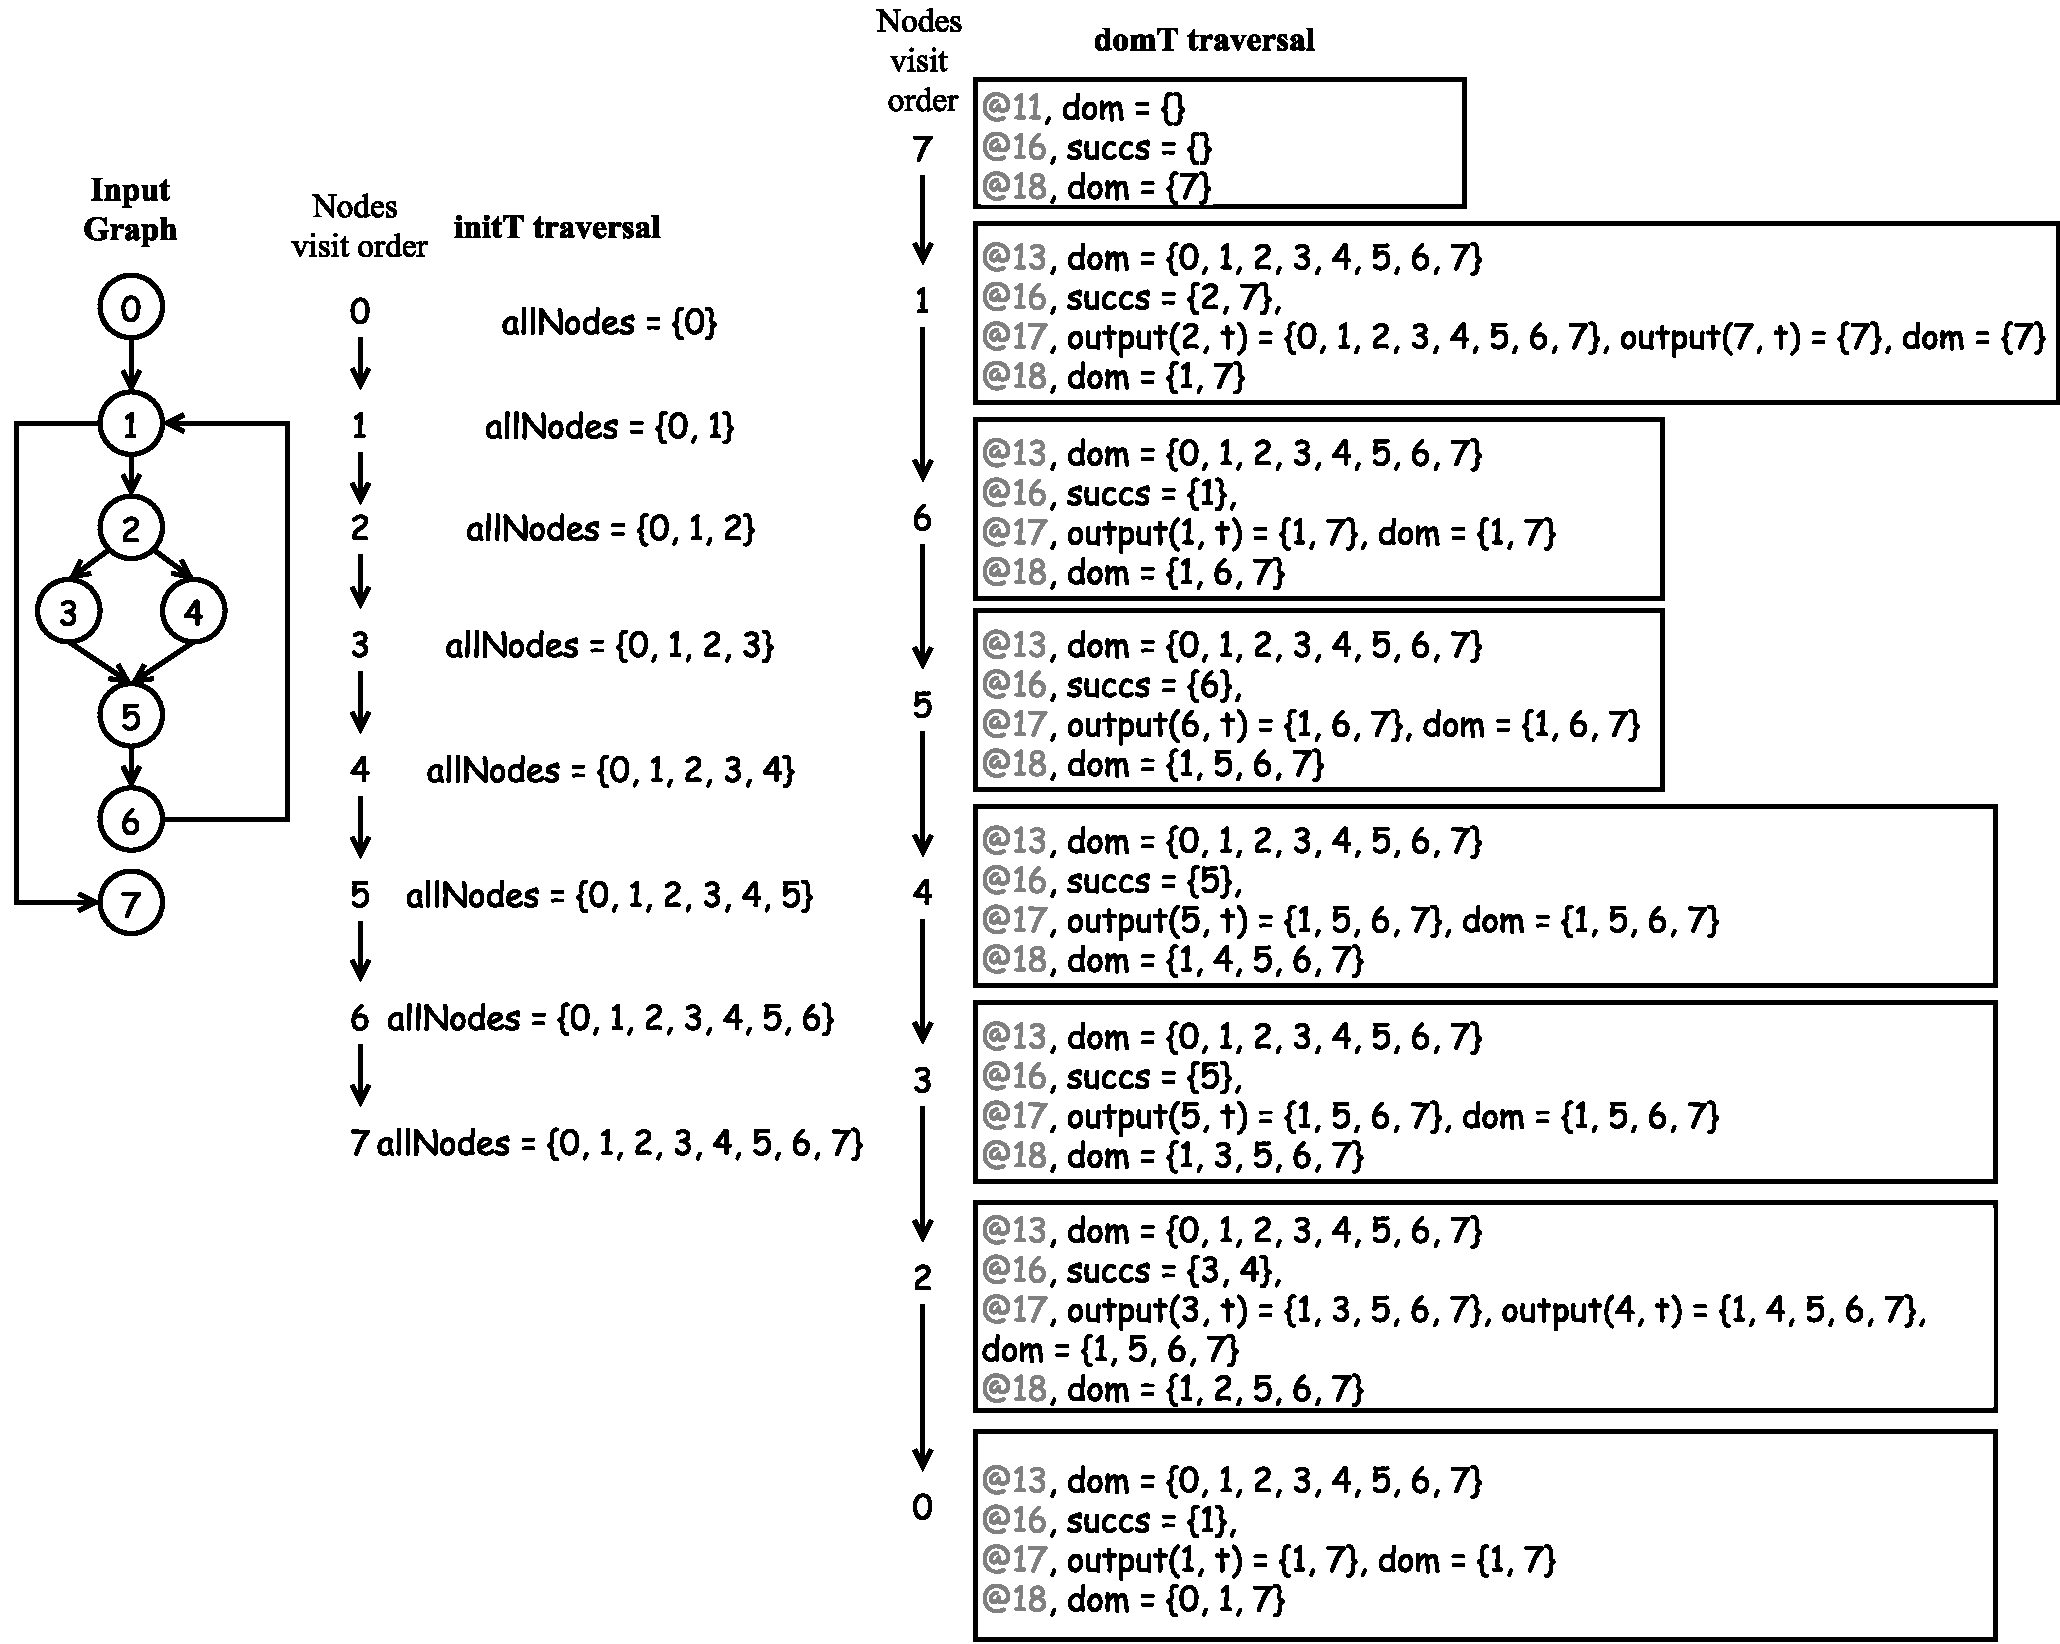
\includegraphics[width=0.9\linewidth]{figures/running-example.pdf}
\caption{Running example of applying the post dominator analysis on an input
graph containing branch and loop.}
\label{fig:running-example}
\end{figure}



\fignref{fig:running-example} takes an example graph, and shows the results of
\lstinline|initT| and \lstinline|domT| traversals. Our example graph is a CFG
containing seven nodes with a branch and a loop. The \lstinline|initT| traversal
visits nodes sequentially and adds node id to the collection
\lstinline|allNodes|. The \lstinline|domT| traversal visits nodes in the
post-order\footnote{The traversal strategies chosen for \lstinline|initT| and
\lstinline|domT| traversals is explained in \secnref{subsec:example}.} and
computes a set of nodes that post dominate every visited node (as indicated by
the set of node ids). For instance, node 7 is post dominated by itself, hence
the output at node 7 is \{7\}.
In \fignref{fig:running-example}, under \lstinline|domT| traversal, for each
node visited, we show the key intermediate steps indicated by $@$ line number.
These line numbers correspond to the line numbers shown in Listing
\ref{lst:dominators}. We will explain the intermediate results while visiting
node 2. In the \lstinline|domT| traversal, at line 13, the output set
\lstinline|dom| is initialized using \lstinline|allNodes|, hence \lstinline|dom|
= \{0, 1, 2, 3, 4, 5, 6, 7\}. At line 16, node 2 has two successors: \{3, 4\}.
At line 17, the set \lstinline|dom| is updated by performing an
\lstinline|intersection| operation using the outputs of successors 3 and 4. The
output of 3 and 4 are \{1, 3, 5, 6, 7\} and \{1, 4, 5, 6, 7\} respectively. By
performing the intersection of these two sets, the \lstinline|dom| set becomes
\{1, 5, 6, 7\}. At line 18, the id of the visited node is added to the
\lstinline|dom| set and it becomes \{1, 2, 5, 6, 7\}.
Hence, the post dominator set for node 2 is \{1, 2, 5, 6, 7\}. Similarly,
the post dominator set for other nodes can be calculated.

% 
% 
% \textit{Dominator analysis} written using the traversal constructs is shown in
% Figure \ref{fig:dominator}. The goal of this analysis is to find the dominator
% of each node in the cfg. Initially we have to traverse the cfg to collect all
% the nodes present in the cfg. This is realized by the init traversal in line
% which adds \textit{Dominator analysis} has two traversals - \texttt{init,
% dominator}. Line 24 applies \texttt{init} traversal on control flow graph
% \texttt{g} and the traversal direction is \texttt{FORWARD}, which means
% traversing the graph \texttt{g} from start node to end node. \texttt{init}
% traversal visits every node in the graph \texttt{g} and returns an output of
% type \texttt{int} (Line 2). Line 3 in \texttt{init} traversal has a global
% variable \texttt{allNodes} collecting the node ids. \texttt{init} traversal
% returns the current node's id as output. Line 25 applies \texttt{dominator}
% traversal on graph \texttt{g} and the traversal direction is \texttt{FORWARD}.
% It also takes fixpoint function \texttt{fp} which implies that
% \texttt{dominator} traversal will be called multiple times till the fixpoint is
% reached. Line 8 queries the output of node \texttt{n} associated with
% \texttt{dominator} traversal. If there is no output, it means that this is the
% first time node \texttt{n} is traversed using \texttt{dominator} traversal. So
% we assign \texttt{dom} to \texttt{allNodes} which contains ids of all the nodes.
% If there is output for node \texttt{n} asscoiated with \texttt{dominator}
% traversal, then we assign the output to the \texttt{dom} (Line 10-12). Line
% 13-14 merges the \texttt{dom} with the node \texttt{n}'s predecessor's output
% associated with \texttt{dominator} traversal using the \texttt{intersection}
% operation. Line 15 queries the output of node \texttt{n} associated with
% \texttt{init} traversal and assigns to \texttt{gen} variable. This also implies
% that \texttt{init} traversal should be applied before \texttt{dominator}
% traversal. Line 16-17 adds the \texttt{gen} variable to \texttt{dom} and returns
% it as output.

%\textit{Dominator analysis} written using the traversal constructs is shown in Figure \ref{fig:dominator}. \textit{Dominator analysis} has two traversals - \texttt{init, dominator}. Line 24 applies \texttt{init} traversal on control flow graph \texttt{g} and the traversal direction is \texttt{FORWARD}, which means traversing the graph \texttt{g} from start node to end node. \texttt{init} traversal visits every node in the graph \texttt{g} and returns an output of type \texttt{int} (Line 2). Line 3 in \texttt{init} traversal has a global variable \texttt{allNodes} collecting the node ids. \texttt{init} traversal returns the current node's id as output. Line 25 applies \texttt{dominator} traversal on graph \texttt{g} and the traversal direction is \texttt{FORWARD}. It also takes fixpoint function \texttt{fp} which implies that \texttt{dominator} traversal will be called multiple times till the fixpoint is reached. Line 8 queries the output of node \texttt{n} associated with \texttt{dominator} traversal. If there is no output, it means that this is the first time node \texttt{n} is traversed using \texttt{dominator} traversal. So we assign \texttt{dom} to \texttt{allNodes} which contains ids of all the nodes. If there is output for node \texttt{n} asscoiated with \texttt{dominator} traversal, then we assign the output to the \texttt{dom} (Line 10-12). Line 13-14 merges the \texttt{dom} with the node \texttt{n}'s predecessor's output associated with \texttt{dominator} traversal using the \texttt{intersection} operation. Line 15 queries the output of node \texttt{n} associated with \texttt{init} traversal and assigns to \texttt{gen} variable. This also implies that \texttt{init} traversal should be applied before \texttt{dominator} traversal. Line 16-17 adds the \texttt{gen} variable to \texttt{dom} and returns it as output.

%Live variable analysis written using the traversal constructs is shown in Figure \ref{fig:live-variable}. Line 1 denotes the node properties. Each node has a property called stmt which represents program statements. \textit{Live variable} has three traversal blocks. \textit{kill\_traversal} captures the variables that are defined in the node. In this traversal, output of each node is the variable defined in it, which we call as killed variables in this analysis. In \textit{gen\_traversal}, output of each node is the variable used in it, which we call as generated variables. The \textit{live\_analysis} traversal is the traversal which performs the live variable analysis. This traversal is called with fixpoint function as it is a data flow analysis and runs till the fixpoint is reached. The traverse method calls in line 29, 30, 31 calls the respective traversals passed.
% 
% The next section gives an overview of our approach where we analyse our
% traversal and the input cfg to arrive at the best traversal strategy to traverse
% the graph.


% \section{Dynamic Properties of Graphs}
% \label{sec:dynamic-properties}
% Our approach requires classifying input graphs based on the connectivity of
% nodes.
% \begin{itemize}
%   \item {\em Sequential}: All nodes in the graph have single successor and
%   predecessor.
%   \item {\em Branch}: There exists nodes that have more than one successors or
%   predecessors.
%   \item {\em Loop}: There exists cycle(s) in the graph.
% \end{itemize}

% the nature of the control flow in it. Based on the nature of the control flow we
% classify graphs into:
% \begin{itemize}
%   \item {\em Sequential control flow}: CFG contains no branch instructions and
%   all nodes have single successor.
%   \item {\em Conditional branch control flow}: CFG contains branch instructions,
%   such as \lstinline|if-else|, \lstinline|switch-case|, etc, however no loop
%   instructions, such as \lstinline|for|, \lstinline|while|, etc, exists. 
%   \item {\em Loop based control flow}: CFG contains loop instructions.
%   \begin{itemize}
%     \item {\em With conditional branch}: CFG contains loop instructions and
%     branch instructions. 
%     \item {\em Without conditional branch}: CFG contains loop instructions, but
%     no branch instructions.
%   \end{itemize}
% \end{itemize}

\section{Static and Runtime Properties}
\label{sec:compute-properties}
While it is known in the literature that choosing a right traversal strategy for
the source code analysis can significantly improve the
performance. For example, ~\cite{atkinson2001implementation} have developed a hybridized iterative-worklist algorithm that processes fewer blocks than the traditional algorithm. Despite these advances, how to choose a right traversal
strategy, what factors influence the selection of the right traversal strategy,
what properties of the analysis and graph are important, and how to determine
them, were not known.

In this section, we describe the factors that influence the selection of the
optimal traversal strategy for any given traversal. These factors include: the
static properties of the analysis and the runtime properties of the graph. We
also describe how the challenge of computing these properties is solved with the
help of the constructs and operations proposed in our system of expressing
source code analysis as traversals (\secnref{sec:language}).
% 
% 
% In this section, we describe properties that our technique relies upon and 
% provide algorithms for computing them. 
% Algorithms for computing the static properties requires that the
% analysis traversals are expressed using our system that is described in
% \secnref{sec:language}. 
% While it is conceivable that these properties can be inferred, we leave 
% such inference for future work. 

\subsection{Data-Flow Sensitivity}
The {\em data-flow sensitivity} property of a traversal models the dependence of
the traversal outputs of nodes in the input graph. A traversal is data-flow
sensitive if the output of a node is computed using the outputs of other
nodes. For instance, in the reaching definition data-flow analysis, the outputs
of nodes are computed using the outputs of predecessors and in live variable
data-flow analysis, the outputs of nodes are computed using the outputs of
successors. Hence, both reaching definition and live variable analysis are
data-flow sensitive.

% Data flow sensitivity is a property defined for every traversal in the analysis.
% A traversal is said to be data flow sensitive, if the traversal output of a node
% is computed using the traversal outputs of its neighbors (successors or
% predecessors). 

\begin{definition}\label{def:dataflow}
$P_{DataFlow}$ (\textbf{Data-flow sensitivity}).\ Given a traversal
\lstinline|t| with body \lstinline|tbody|, a map $O$ that collects and maintains
the traversal output of nodes ($O$ is indexed using node ids), and $F$, a
function representing the computation of $O[.]$ in the traversal body
\lstinline|tbody|, if for any node $n$, its output $O[n]$ is computed by
applying $F$ over one or more of $O[n']$, where $n' \neq n$, then \lstinline|t|
is data-flow sensitive. That is $P_{DataFlow}$ is \textit{true} otherwise
\textit{false}.
\end{definition}
% 
% A traversal is data flow sensitive, if
% \begin{equation}
% O[n] = F(O[n'])
% \end{equation}

For instance, consider the lines 16 and 17 of the \lstinline|domT| traversal
shown in Listing \ref{lst:dominators}. Here, a variable \lstinline|dom| holds
the traversal output of a node $n$ and it is computed by applying an
\lstinline|intersection| operation on the traversal outputs of successors of
$n$. Here, the function $F$ is \lstinline|intersection| over the outputs of all
successors of a node.

\begin{algorithm}[ht!]
\caption{Algorithm to detect data-flow sensitivity}
\label{algo:flow-sensitive}
\KwIn{\lstinline|t := traversal(n : Node) : T \{ tbody \}|}
\KwOut{\textit{true/false}}
$A$ $\leftarrow$ \textit{getAliases}(\lstinline|tbody|, \lstinline|n|)\;
\ForEach{ \lstinline|stmt| $\in$ \lstinline|tbody|}{
	\If{$stmt$ $=$ \lstinline|output(n', t')|}{
		\If{\lstinline|t'| $==$ \lstinline|t| and \lstinline|n'| $\notin$ $A$ }{
			return \textit{true}\;
		}
	}
	
}
return \textit{false}\;
\end{algorithm}

\subsection{Computing Data-Flow Sensitivity}
\label{sec:df-algo}
To determine the data-flow sensitivity property of a traversal, the operations
performed in the traversal needs to be analyzed to check if the output of a
node is computed using the outputs of other nodes. In our system of expressing
analysis as traversals, the only way to access the output of a node is via
\lstinline|output()| expression, hence given a traversal \lstinline|t| :=
\lstinline|traversal(n : Node)| :
\lstinline|T| \{ \lstinline|tbody| \} as input, \algoref{algo:flow-sensitive}
parses the statements in the traversal body \lstinline|tbody| to identify method
calls of the form \lstinline|output(n', t')| that fetches the output of a node
\lstinline|n'| in the traversal \lstinline|t'|. If such method calls exists,
they are further investigated to determine if \lstinline|n'| does not point to
\lstinline|n| and \lstinline|t'| points to \lstinline|t|.
If such method calls exists, it means that the traversal output for the current
node \lstinline|n| is computed using the traversal outputs of other nodes
(\lstinline|n'|) and hence the traversal is data-flow sensitive.
For performing the points to check, \algoref{algo:flow-sensitive} assumes that
an alias environment is computed by using must alias
analysis~\cite{must-alias}. \algoref{algo:flow-sensitive} requires that
the must alias analysis computes all names in the \lstinline|tbody| that must
alias each other at any program point. The must alias information ensures that
\algoref{algo:flow-sensitive} never classifies a data-flow sensitive traversal
as data-flow insensitive.
A \lstinline|tbody| may contain more than one \lstinline|output()| statement,
however \algoref{algo:flow-sensitive} requires only one \lstinline|output()|
statement that fetches the output of other nodes than the current node, to
classify the traversal as data-flow sensitive. The control and loop statements
in the \lstinline|tbody| do not have any impact on \algoref{algo:flow-sensitive}
for computing the data-flow sensitivity property.

\subsection{Loop Sensitivity}
The loop sensitivity property models the effect of the loops in the input graph.
If an input graph contains loops and if the traversal is affected by the loop,
the traversal may require multiple iterations to compute the output of nodes.
In the multiple iterations, the traversal outputs of nodes either shrinks or
expands to reach a fixpoint. Hence, we define a traversal as loop sensitive,
if the traversal output of nodes in subsequent iterations shrinks or expands.

\begin{definition}\label{def:loop-sensitivity}
$P_{Loop}$ (\textbf{Loop sensitivity}). Given a traversal \lstinline|t|, a map
$O$ that collects and maintains the traversal output of nodes ($O$ is indexed
using node ids), and $O^i[n]$ represents the output of node $n$ in the $i^{th}$
iteration, if $O^{i+1}[n]$ $\lll$ $O^{i}[n]$ or $O^{i+1}[n]$ $\ggg$ $O^{i}[n]$,
then $t$ is loop sensitive, i.e. $P_{Loop}$ is \textit{true} otherwise
\textit{false}.
The relation $\lll$ represents \lstinline|shrink| and it is given by,
$O^{i+1}[n]$ $\lll$ $O^{i}[n]$, if $|O^{i+1}[n]|$ $<$ $|O^{i}[n]|$, and the
relation $\ggg$ represents \lstinline|expand| and it is given by, $O^{i+1}[n]$
$\ggg$ $O^{i}[n]$, if $|O^{i+1}[n]|$ $>$ $|O^{i}[n]|$, where $|C|$ is the
cardinality of the output collection $C$.
\end{definition}

Since the loop sensitivity property is defined only for data-flow sensitive
traversals, we know that the traversal output of nodes in each iteration is
computed using the traversal output of other nodes (possible neighbors), we have
$O^{i}[n]$ = $F(O^{i}[n'])$ and $O^{i+1}[n]$ = $F(O^{i+1}[n'])$, where $n$, $n'$
are any two nodes such that $n' \neq n$. By substituting these in the
\lstinline|shrink| relation $O^{i+1}[n]$ $\lll$ $O^{i}[n]$, we get,
$F(O^{i+1}[n'])$ $\lll$ $F(O^{i}[n'])$. For this relation to be
\lstinline|true|, 1) the output of any node $n'$ in any two subsequent
iterations $i$ and $i+1$ must shrink and 2) the function $F$ has the shrink
property. Similarly, for expand relation, 3) the output of any node $n'$ in any
two iterations $i$ and $i+1$ must expand and 4) the function $F$ has the expand
property.
As we know $F$ represents the function in the traversal body that computes the
outputs of nodes, if $F$ has the property of shrink or expand, then the
traversal can be classified as loop sensitive.
% 
% 
% To summarize, for the traversal output of any node to shrink between any two
% subsequent iterations, the traversal outputs of neighbor (predecessors or
% successors) must also shrink in the subsequent iterations, and the functions
% applied must have the shrink property. Similarly, for the traversal output of
% any node to expand between any two subsequent iterations, the traversal outputs
% of neighbor (predecessors or successors) must also expand in the subsequent
% iterations, and the functions applied must have the expand property.
% 
% 
% and for this to be true, $O^{i+1}[n']$ $\lll$ $O^{i}[n']$ and $F(O^{i}[n'])$
% $\lll$ $O^{i}[n']$. Similarly, $O^{i+1}[n']$ $\ggg$ $O^{i}[n']$ and
% $F(O^{i}[n'])$ $\ggg$ $O^{i}[n']$ holds for the expand case.

% \begin{definition}\label{def:loop-sensitivity}
% $P_{Loop}$ (\textbf{Loop sensitivity}) is a property of a data flow
% sensitive traversal that indicates whether the data flow in the traversal
% is affected by the loops (or cycles) present in the input graph. 
% The domain of values for $P_{DataFlow}$ are \{\textit{true}, \textit{false}\}.
% If a traversal is affected by the loops in the graph, the traversal requires
% multiple iterations to compute output for nodes.
% The traversal output either shrinks or expands before reaching a fixpoint, if
% it is affected by the loops. Hence, if the traversal output shrinks or expands
% in the subsequent iterations, then the traversal is said to be loop sensitive.
% If $O[n, i]$ represents the traversal output of a node $n$ in iteration $i$, and
% if $O[n, i+1]$ $\lll$ $O[n, i]$ or $O[n, i+1]$ $\ggg$ $O[n, i]$, then $P_{Loop}$
% = \textit{true}. The symbol $\lll$ represents \lstinline|shrink| and the symbol
% $\ggg$ represents \lstinline|expand|. 
% \end{definition}
% 
% Loop sensitivity is defined for only the data flow sensitive traversals (data
% flow insensitive traversals do not have loop sensitivity property). When the
% input graph contains loops, the traversal may or may not get affected by it. If
% a traversal gets affected by the loops in the input graph, the traversal visits
% nodes multiple times (requires multiple iterations) to stabilize the output and
% reach a fix-point. To determine this statically, we assume that the traversal
% takes multiple iterations (visits nodes multiple times), and we check if the
% traversal output of nodes expands or shrinks in the subsequent iterations. If
% the traversal output expands or shrinks in the subsequent iterations, we can
% conclude that the traversal will get affected by the loops in the input graph.
% The expand and shrink conditions are given by:  $O[n, i+1]$ $\lll$ $O[n, i]$ and
% $O[n, i+1]$ $\ggg$ $O[n, i]$. For these conditions to hold, the conditions below
% must also be true. \\
% 
% When the input graph contains loops, the traversal visits nodes multiple times
% to stabilize the output and reach a fix-point. A traversal is checked for loop
% sensitivity if the traversal is data flow sensitive, hence following conditions
% holds for a traversal to be loop sensitive: \\
% 
% $F(O[n_p]) \lll O[n_p]$ $\wedge$ $O[n_p, i+1] \lll O[n_p, i]$ $\Rightarrow$
% $O[n, i+1] \lll O[n, i]$ \\
% $F(O[n_p]) \ggg O[n_p]$ $\wedge$ $O[n_p, i+1] \ggg O[n_p, i]$ $\Rightarrow$
% $O[n, i+1] \ggg O[n, i]$, where $n_p \in n.preds$ or $n_p \in n.succs$. \\

To give an example, consider the \lstinline|domT| traversal shown in Listing
\ref{lst:dominators}. Since \lstinline|domT| is data-flow sensitive, we can
check the loop sensitivity property. There are two functions that contributes to
the traversal output of any node $n$ in \lstinline|domT| traversal body. These
are \lstinline|intersection| (line 16) and \lstinline|add| (line 17). For
\lstinline|domT| to be loop sensitive, we require that both
\lstinline|intersection| and \lstinline|add| have either shrink or expand
property. However, \lstinline|intersection| has the shrink property and
\lstinline|add| has the expand property, hence we cannot classify
\lstinline|domT| to be loop sensitive.

%\begin{wrapfigure}{R}{.5\textwidth}
\begin{algorithm}
\caption{Algorithm to detect loop sensitivity}
\label{algo:loop-sensitive}
\begin{multicols}{2}
\KwIn{\lstinline|t := traversal(n: Node) : T \{ tbody \}|}
\KwOut{\textit{true/false}}
$V$ $\leftarrow$ \{\} // a set of output variables related to n\;
$V'$ $\leftarrow$ \{\} // a set of output variables not related to n\; 
\lstinline|expand| $\leftarrow$ \textit{false}\; 
\lstinline|shrink| $\leftarrow$ \textit{false}\;
\lstinline|gen| $\leftarrow$ \textit{false}\; 
\lstinline|kill| $\leftarrow$ \textit{false}\;
$A$ $\leftarrow$ \textit{getAliases($n$)}\; 
\ForEach{ \lstinline|stmt| $\in$ \lstinline|tbody| }{
	\If{ \lstinline|stmt| is \lstinline|v| = \lstinline|output|($n'$,
	$t'$)}{ \If{$t'$ $==$ \lstinline|t|}{
			\eIf{$n'$ $\in$ $A$}{
				$V$ $\leftarrow$ $V$ $\cup$ \textit{\lstinline|v|}\;
			}{
				$V'$ $\leftarrow$ $V'$ $\cup$ \textit{\lstinline|v|}\;					
			}
		}
	}
}
\ForEach{ \lstinline|stmt| $\in$ \lstinline|tbody| }{
		\If{ \lstinline|stmt| $=$ \lstinline|union|($c_1$, $c_2$) }{
			\If{ ($c_1$ $\in$ $V$ and $c_2$ $\in$ $V'$) $||$ ($c_1$ $\in$ $V'$ and $c_2$
			$\in$ $V$)}{ 
				\lstinline|expand| $\leftarrow$ \textit{true}\; 
			}
		}
		\If{ \lstinline|stmt| $=$ \lstinline|intersection|($c_1$, $c_2$)}{
			\If{($c_1$ $\in$ $V$ and $c_2$ $\in$ $V'$) $||$ ($c_1$ $\in$ $V'$
			and $c_2$ $\in$ $V$)}{ 
				\lstinline|shrink| $\leftarrow$ \textit{true}\;
			}
		}
		\If{ \lstinline|stmt| $=$ \lstinline|add|($c_1$, $e$) $||$	
		\lstinline|addAll|($c_1$, $c_2$)}{ 
			\If{$c_1$ $\in$ $V$}{ 
				\lstinline|gen| $\leftarrow$ \textit{true}\; 
			}
		}
		\If{ \lstinline|stmt| $=$ \lstinline|remove|($c_1$, $e$) $||$
		\lstinline|removeAll|($c_1$, $c_2$)}{ 
			\If{$c_1$ $\in$ $V$}{ 
				\lstinline|kill| $\leftarrow$ \textit{true}\;
			}
		}
}
\eIf{ (\lstinline|expand| and \lstinline|gen|) $||$ (\lstinline|shrink| and
\lstinline|kill|) }{ return \textit{true}\;
}{
	return \textit{false}\;
}
\end{multicols}
\end{algorithm}
%\end{wrapfigure}
\subsection{Computing Loop Sensitivity}
\label{sec:ls-algo}
In general, computing the loop sensitivity property statically is challenging in
the absence of an input graph, however the constructs and operations of our
system enables static inference of this property.

A traversal is loop sensitive, if the output of any node in any two subsequent
iterations either shrinks or expands. 
To determine if the traversal output expands or shrinks in the subsequent
iterations, the operations performed in the traversal needs to be analyzed.
\tabref{tab:operations} provides several operations that can be performed on the
traversal outputs. The operations \lstinline|add|, \lstinline|addAll|,
and \lstinline|union| always expands the output and the operations
\lstinline|remove|, \lstinline|removeAll|, and \lstinline|intersection| always
shrinks the output.
% 
% A combination of operations like \lstinline|union| with \lstinline|add| suggests
% that the traversal output expands, and a combination of operations like
% \lstinline|intersection| with \lstinline|remove| suggests that the traversal
% output shrinks. 
% We provide an algorithm to determine this property by analyzing the operations
% performed in the traversal body in \algoref{algo:loop-sensitive}.
% The key idea of our algorithm to determine loop sensitivity is as follows: When
% the input graph contains a loop, a traversal may visit nodes multiple times,
% until a fixpoint is reached (where the output of nodes do not change further).
% {\em Our key observation is that, for traversal output to get affected by the
% loops present in the input graph, output of nodes in multiple iterations either
% expands or shrinks}. It is possible to determine statically, whether the output
% of nodes in multiple iterations either shrinks or expands by investigating the
% operations used in the traversal body. Operations like \lstinline|add|,
% \lstinline|addAll|, \lstinline|union|, etc, always expands the output, and
% operations like \lstinline|remove|, \lstinline|removeAll|,
% \lstinline|intersection|, always shrinks the output. 

Given a traversal \lstinline|t| := \lstinline|traversal(n : Node)| :
\lstinline|T| \{ \lstinline|tbody| \}, \algoref{algo:loop-sensitive} determines
the loop sensitivity of \lstinline|t|.
\algoref{algo:loop-sensitive} investigates the statements in the
\lstinline|tbody| to determine if the traversal outputs of nodes in multiple
iterations either expands or shrinks. For doing that, first it parses the
statements to collect all output variables related and not related to input node
\lstinline|n| using the must alias information as in
\algoref{algo:flow-sensitive}. This is determined in lines 8-14, where all
output variables are collected (output variables are variables that gets
assigned by the \lstinline|output| operation) and added to two sets $V$ (a set
of output variables related to n) and $V'$ (a set of output variables not
related to n).
Upon collecting all output variables, \algoref{algo:loop-sensitive} makes
another pass over all statements in the \lstinline|tbody| to identify six kinds
of operations: \lstinline|union|, \lstinline|intersection|, \lstinline|add|,
\lstinline|addAll|, \lstinline|remove|, and \lstinline|removeAll|. These
operations are defined in \tabref{tab:operations}\footnote{The operations not
listed here do not expand or shrink the output.}.
In lines 16-18, the algorithm looks for \lstinline|union| operation, where one
of the variables involved is an output variables related to \lstinline|n| and
the other variable involved is not related to \lstinline|n|. These conditions
are simply the true conditions for the data-flow sensitivity, where the output
of the current node is computed using the outputs of other nodes (neighbors).
Similarly, in lines 19-21, the algorithm looks for \lstinline|intersection|
operation. The lines 22-27, identifies add and remove operations that adds or
removes elements from the output related to node \lstinline|n|. Finally, if
there exists \lstinline|union| and \lstinline|add| operations, the output of a
node always expands, and if there exists \lstinline|intersection| and
\lstinline|remove| operations, the output of a node always shrinks. For a
data-flow traversal to be loop sensitive, the output of nodes must either expand
or shrink, not both (lines 28-29). 

\subsection{Graph \Graphprop}
So far we have described the two static properties of the analysis that
influences the traversal strategy selection. A property of the input graph
also influences the selection. This property is the \graphprop{} in the
graph. Based on the \graphprop{}, we classify graphs into four categories:
\{sequential, branch only, loop w/o branch, loop w/ branch\}. In case of
sequential graphs, all nodes in the graph have no more than one successor and
predecessor. In case of graphs with branches, nodes may have more than one
successor and predecessor. In case of graphs with loops, there exists cycles in
the graph. The graph \graphprop{} is determined during the construction of the
graph.

In a source code analysis, traversal output of nodes may depend on each other.
For instance, in forward data-flow analysis, output of a node is computed using
the outputs of its predecessors. Similarly, in the backward data-flow analysis,
output of the successors is required.
Graph cyclicity plays an important role in the selection of the appropriate
traversal strategy. In case of graphs with branches and loops, the outputs of
all dependent nodes of a node (predecessors or successors) may not be available
at the time of visiting the node, hence a traversal strategy must be selected
that guarantees that the outputs of all dependent nodes of a node are available
prior to computing the node's output. 

% 
% output of the predecessors of a node
% flows to the node and it is consumed to construct the output of the node.
% Similarly, in the backward control flow analysis, output of the successors
% of a node flows to the node. 
% Also, the output of all dependent nodes of a node (predecessors or successors)
% may not be available at the time of visiting the node in case of graphs with
% branches and loops. For this reason, a traversal may take multiple iterations to
% correctly compute and propagate the results. Hence, the graph \graphprop{} plays
% an important role in selecting an appropriate order of visiting the nodes (the
% traversal strategy), such that output of the dependent nodes are available for
% computing the output of a node.

% 
% The graph connectivity property is determined during the construction of the
% graph. If every node in the graph has single successor and predecessor, the
% graph is said to have sequential connectivity. If there exists nodes with more
% than one successors and predecessors, then the graph has branch connectivity. If
% there exists a node in the graph that can reach itself by traversing in the
% forward direction (via successors), the graph is said to have loop connectivity.

% \begin{table}[ht!]
\caption{Traversal strategies}
\label{tab:strategies}
\begin{tabular}{c|c}
Traversal stategy & Description \\\hline\hline
\textit{SEQ} & Sequential order \\\hline
\textit{INC} & Increasing order of node ids \\\hline
\textit{DEC} & Decreasing order of node ids \\\hline 
\textit{PO} & Post order \\\hline
\textit{RPO} & Reverse post order \\\hline 
\textit{WPO} & Worklist with post order \\\hline
\textit{WRPO} & Worklist with reverse post order \\\hline
\end{tabular}
\end{table}

\section{Traversal Strategies - Candidates}
\label{sec:candidates}

We have picked seven traversal strategies as candidates for choosing an optimal
traversal strategy for given a traversal and an input graph. The selected candidate strategies were arrived at by carefully reviewing compilers textbooks, implementations, and source code analysis frameworks. We also made sure that the selected candidate strategies are applicable to any graphs and analysis. We did not consider strategies like chaotic iteration based on Weak Topological Ordering because they are effective only for computing fixed points of continuous function over lattices of infinite height ~\cite{bourdoncle93}.
The selected traversal strategies are describe below:
\begin{itemize}
  \item \textbf{Any order (\textit{ANY})}: In this traversal strategy, nodes can
  be visited in any order. In our implementation, we visit the nodes in the
  order they appear in the nodes list $N$ (\defref{def:cfg}).
  \item \textbf{Increasing order of node ids (\textit{INC})}: In this traversal
  strategy, the nodes are visited in the increasing order of their node ids. The
  node ids are assigned during the construction of the graph. For instance, while
  constructing a CFG, the node ids are assigned in the control flow order. 
%   
%   of their control flow. During the
%   construction of the CFG, the nodes are created and assigned ids based on their
%   control flow order.
  \item \textbf{Decreasing order of node ids (\textit{DEC})}: In this traversal
  strategy, the nodes are visited in the reverse order of their node ids
  (decreasing order of node ids).
  \item \textbf{Post-Order (\textit{PO})}: In this traversal, the successors of
  any node are visited before visiting the node.
  \item \textbf{Reverse Post-Order (\textit{RPO})}: In this traversal, the
  predecessors of any node are visited before visiting the node.
  \item \textbf{Worklist with Post-Order (\textit{WPO})}: In this traversal, the
  nodes are visited in the order they appear in the worklist. A worklist is a
  data structure used to keep track of nodes to be visited. In WPO, worklist is
  initialized with post-ordering of nodes. The worklist is maintained as
  follows: whenever a node from the worklist is removed and visited, all its
  successors (for forward traversals) or predecessors (for backward traversals)
  are added to the worklist as done in~\cite{atkinson2001implementation}.
  \item \textbf{Worklist with Reverse Post-Order (\textit{WRPO})}: In this
  traversal, the nodes are visited in the order they appear in the worklist. The
  worklist is initialized with nodes in the reverse post-order.
\end{itemize}

\begin{figure}[ht!]
\centering
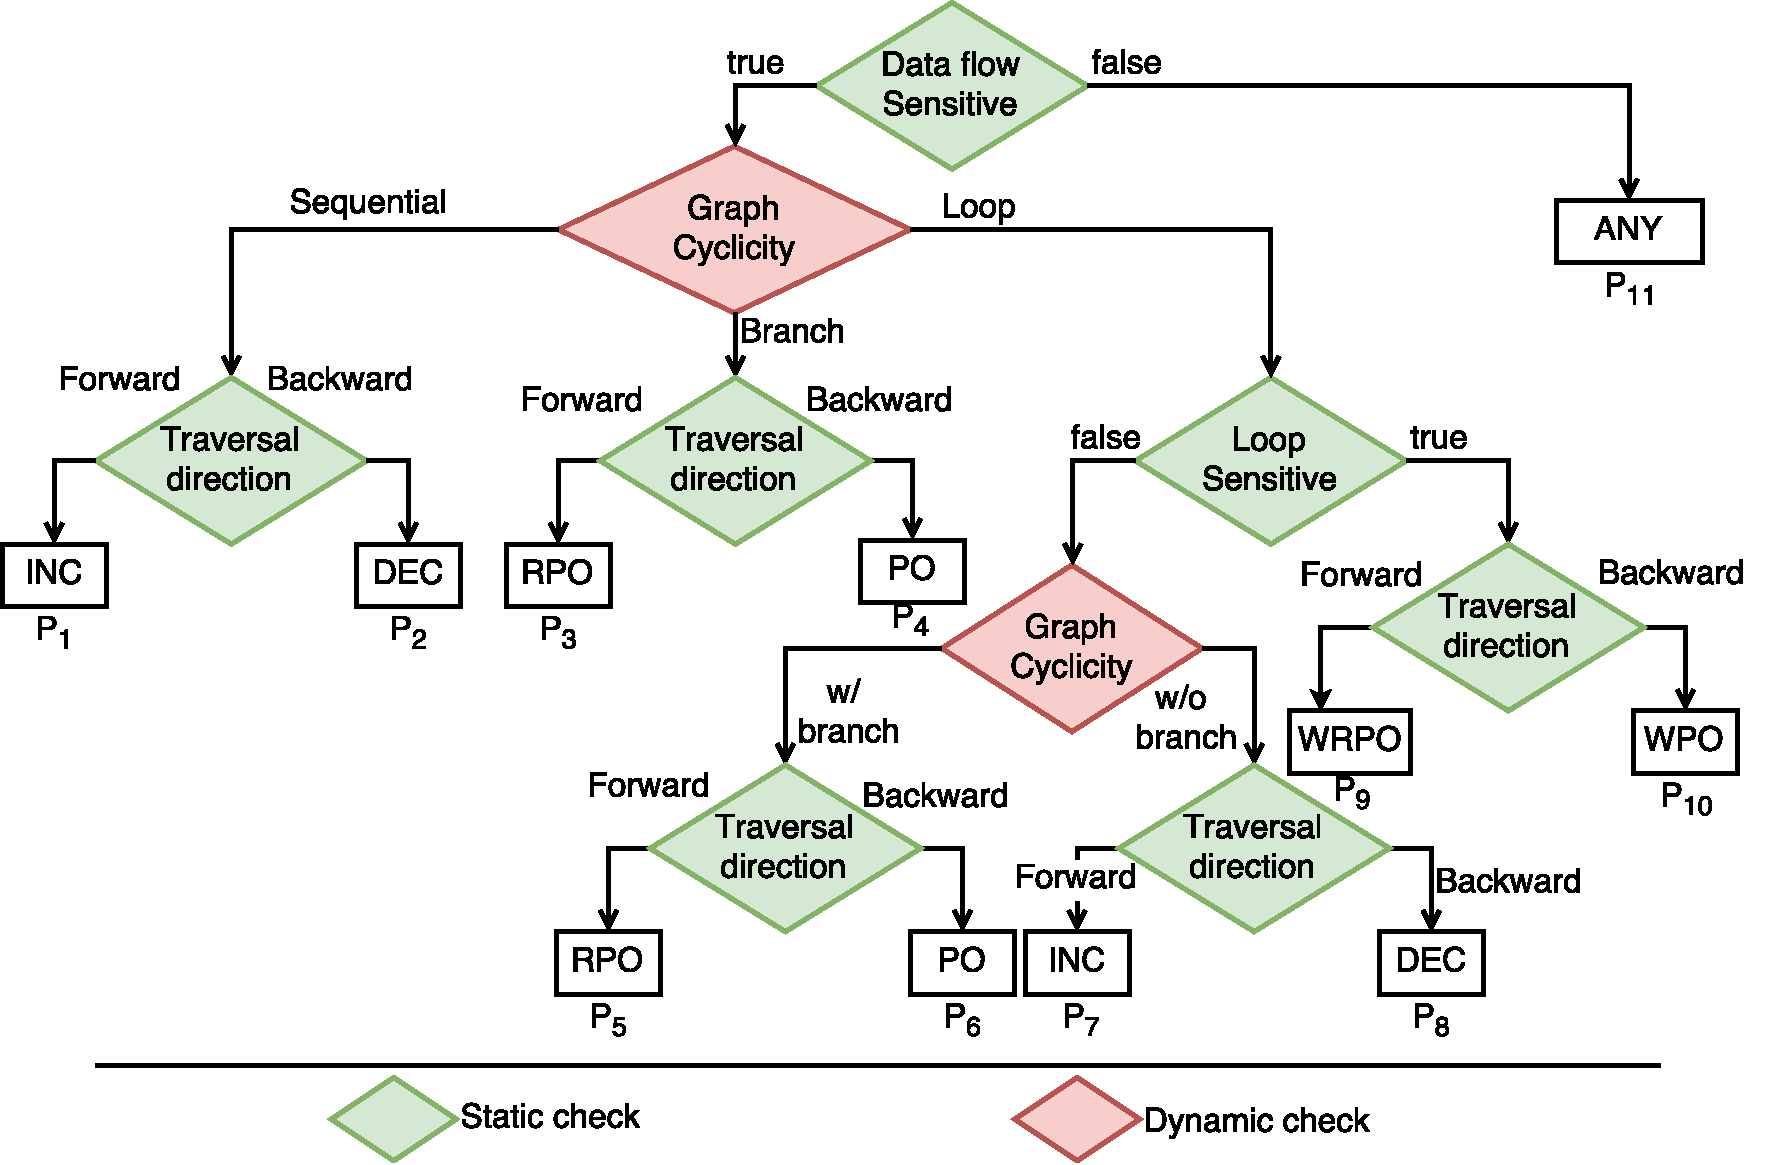
\includegraphics[width=1\linewidth]{figures/decision.pdf}
\caption{Traversal strategy selection decision tree.}
\label{fig:decision-diagram}
\end{figure}

\section{Decision Tree for Traversal Strategy Selection}
\label{sec:decision-tree}
At this point, we know the factors that influence the traversal strategy
selection: the static properties of the analysis, and the runtime property of
the graph. Our goal is to check these properties in certain order to quickly
decide the best traversal strategy for a given analysis and a graph, such that
only relevant properties are checked and the overhead of static/runtime check is
minimized\footnote{Our evaluation shows that the overhead is less than 0.2\% 
of the total running time for a large dataset and less than 0.01\% for an ultra-large dataset.}.
To that end, we carefully devised a decision tree as shown in
\fignref{fig:decision-diagram} for traversal strategy selection.

%\fignref{fig:decision-diagram} shows our decision tree for traversal strategy selection. 
The leaf nodes of the tree are one of the seven traversal strategies
and non-leaf nodes are static/runtime checks. The decision tree has eleven paths
marked $P_1$ through $P_{11}$. Given a traversal and an input graph, one of the
eleven paths will be taken to decide the best traversal strategy. The longest
paths $P_5$, $P_6$, $P_7$, and $P_8$ requires five checks and the shortest path
$P_{11}$ requires only one check. The static checks are marked green and the
runtime checks are marked red. The static properties that are checked are:
data-flow sensitivity ($P_{DataFlow}$), loop sensitivity ($P_{Loop}$), and
traversal direction. The runtime property that is checked is the graph
\graphprop{}: sequential, branch, loop w/ branch, and loop w/o branch. We now
provide rationale for arranging the decision tree as shown in
\fignref{fig:decision-diagram}.

The first property that is checked is the data-flow sensitivity of the
traversal. This is a static property determined by analyzing the traversal that
indicates whether the traversal output of any node is dependent on the traversal
output of its neighbors (successors or predecessors). This property is defined
in \defref{def:dataflow} and an algorithm to compute this property is given in
\algoref{algo:flow-sensitive}. The rationale for checking this property first is
that, if a traversal is data-flow insensitive ($P_{DataFlow}$ is
\textit{false}), irrespective of the type of the input graph, the traversal
can finish in a single iteration (no fixpoint computation is necessary). In
such cases, visiting nodes in any order will be efficient, hence we assign
any order (\textit{ANY}) traversal strategy (path $P_{11}$).

For traversals that are data-flow sensitive ($P_{DataFlow}$ is \textit{true}),
further checks are performed to determine the best traversal strategy. Next
property that is checked is the input graph \graphprop{}.
This is because the loop sensitive property is applicable to only graphs with
loops. 
\begin{itemize}
  \item \textit{Sequential Graphs (paths $P_1$ and $P_2$)}:
  In this type of graphs, no branches or loops exists, and all nodes have
  a single successor and predecessor.
  At this point, we know that the traversal is data-flow sensitive and it
  requires output of the neighbors to compute the output for any node. As
  sequential graphs have only one neighbor (successor or predecessor), a
  traversal strategy that visits the neighbor prior to visiting any node is
  sufficient to produce an optimal traversal order. To determine which neighbor
  (successor or predecessor), we check the traversal direction property. For
  \lstinline|FORWARD| traversal direction, predecessor of the node must be
  visited before the node and for \lstinline|BACKWARD| traversal direction,
  successor of the node must be visited before the node. These two traversal
  orders are provided by our \textit{INC} and \textit{DEC} traversal
  strategies. The corresponding paths in the decision tree are: $P_1$ and $P_2$.
  \item \textit{Graphs with branches (paths $P_3$ and $P_4$)}:
  In this type of graphs, branches exists, however loops don't exists, which
  means that a node may have more than one successor or predecessor. At this
  point, we know that our traversal is data-flow sensitive and it requires
  output of all neighbors (successors or predecessors) to compute the output for
  any node, we need a traversal order that ensures that all successors and
  predecessors are visited prior to visiting any node. This traversal order is
  given by the post-order (\textit{PO}) and reverse post-order (\textit{RPO})
  traversal strategies. To pick between \textit{PO} and \textit{RPO}, we check
  the traversal direction.
  For \lstinline|FORWARD| traversal direction, we need to visit all predecessors
  of any node prior to visiting the node, hence we pick the \textit{RPO}
  traversal strategy. For \lstinline|BACKWARD| traversal direction, we need to
  visit all successors of any node prior to visiting the node, hence we pick the
  \textit{PO} traversal strategy.
  \item \textit{Graphs with loops (paths $P_5$ to $P_{10}$)}: In this type of
  graphs, loops exists and in addition branches may also exists. We first need
  to check if the traversal is sensitive to the loop (the loop sensitive
  property). At this point, we know that our analysis is data-flow sensitive and
  the input graph has loop based control flow.
  	\begin{itemize}
	\item \textit{Loop sensitive (paths $P_9$ and $P_{10}$)}: When the traversal is
	loop sensitive, for correctly propagating the output, the traversal visits
	nodes multiple times until a fix point condition is satisfied (user may
	provide a fix point function). No iterative traversal strategy can guarantee
	that fix point will be reached in a single traversal of the nodes, hence we
	adopt a worklist based traversal strategy that visits only required 
	nodes (property of the worklist strategy). The worklist traversal strategy
	requires that the worklist (a data structure) is initialized with nodes.
	For picking the best order of nodes for initialization, we further investigate
	the traversal direction. We know that, for \lstinline|FORWARD| traversal
	direction, \textit{RPO} traversal strategy gives the best order of nodes and for
	\lstinline|BACKWARD| traversal direction, \textit{PO} traversal strategy gives
	the best order of nodes, we pick worklist strategy with reverse post-order
	\textit{WRPO} for \lstinline|FORWARD| and worklist strategy with post-order
	\textit{WPO} for \lstinline|BACKWARD| traversal directions.
	 \item \textit{Loop insensitive (paths $P_5$ to $P_8$)}: When the traversal is
	 loop insensitive, the selection problem reduces to the sequential and branch case
	 that is discussed previously, because for loop insensitive traversal, the
	 loops in the input graph is irrelevant and what remains relevant
	 is the existence of the branches.
  	\end{itemize}
\end{itemize}

\subsection{An Example}
\label{subsec:example}
In this section we explain the decision tree using an example source code analysis
and a graph.
The example analysis that we choose is the {\em Post Dominator Analysis} shown
in Listing \ref{lst:dominators} and the graph that we choose is shown in
\fignref{fig:running-example}.
The \textit{Post Dominator Analysis} contains two traversals: \lstinline|initT|
and \lstinline|domT|. 
The \lstinline|initT| traversal is data-flow insensitive ($P_{DataFlow}$ is
\textit{false}) and loop insensitive ($P_{Loop}$ is \textit{false}). The
\lstinline|domT| traversal is data-flow sensitive ($P_{DataFlow}$ is
\textit{true}) and loop insensitive ($P_{Loop}$ is \textit{false}). The
traversal directions of \lstinline|initT| and \lstinline|domT| are
\lstinline|ITERATIVE| and \lstinline|BACKWARD| respectively. 
Our example graph shown in \fignref{fig:running-example} has branches and loops, 
meaning the graph has nodes with more than one successor or
predecessor and has cycles.
% 
% 
% For \lstinline|initT| traversal, $P_{DataFlow}$ is
% \textit{false} and $P_{Loop}$ is \textit{false}, and for \lstinline|domT|
% traversal, $P_{DataFlow}$ is \textit{true} and $P_{Loop}$ is \textit{false}. The
% traversal directions of \lstinline|initT| and \lstinline|domT| traversals are
% \lstinline|ITERATIVE| and \lstinline|BACKWARD| respectively. The connectivity of
% input graphs can be anything in the set \{sequential, branch only, loop w/o
% branch, loop w/ branch\}. We now select an optimal traversal strategy for each
% of them.

For selecting the best traversal strategies for \lstinline|initT| and the graph
with loops and branches, we check the data-flow sensitivity property of the
traversal.
As \lstinline|initT| is data-flow insensitive, \textit{ANY} traversal strategy
is picked as shown by the path $P_{11}$ in \fignref{fig:decision-diagram} and no
further checks are required. The traversal strategy \textit{ANY} represents
nodes visited in any order.

For selecting the best traversal strategies for \lstinline|domT| and the graph
with branch and loop, we check the data-flow sensitivity property of the
traversal.
As \lstinline|domT| is data-flow sensitive, the next property to be checked is
the graph \graphprop{}. As our input graph has loops, the next property to be
checked is whether \lstinline|domT| is loop sensitive ie sensitive to the loops
present in the graph. Since \lstinline|domT| is loop-insensitive, we ignore the
loops present in the graph and investigate the rest of the graph structure. As
our graph contains branches, the next property to be checked is the traversal
direction. The traversal direction for \lstinline|domT| is \lstinline|BACKWARD|,
we pick \textit{PO} traversal strategy for \lstinline|domT| traversal, as shown
by the path $P_6$ in \fignref{fig:decision-diagram}. The traversal strategy
post-order (\textit{PO}) visits all successors of a node before visiting that
node. This is most suitable for backward analysis like \lstinline|domT|, because
backward analysis analyzes successors of a node prior to analyzing the node.

\section{Optimizing the Selected Traversal Strategy}
\label{subsec:optimizations}
The properties of the analysis and the input graph not only helps us select the
best traversal strategy, it also helps to perform several optimizations to the
selected traversal strategies. 

Running an analysis on a cyclic graph may require multiple iterations of the
nodes to compute the fixpoint solution. At least one additional traversal of the
nodes is required before the fixpoint check that compares the result of the last
two traversals to to ensure that results at nodes have stabilized. This
additional traversal and the fixpoint checks at nodes can be eliminated based on
the selected traversal strategy.

For data-flow insensitive traversals, we know that the traversal outputs of
nodes does not depend on the outputs of other nodes, hence both the additional
traversal and the fixpoint checks can be eliminated irrespective of the graph
cyclicity (path $P_{11}$ in our decision diagram
\fignref{fig:decision-diagram}).
In case of data-flow sensitive traversals, the traversal output of a node is
computed using the traversal outputs of other nodes (predecessors or
successors). For data-flow sensitive analysis on a acyclic graph provides an
opportunity to eliminate the additional traversal and fixpoint checks iff the
selected traversal strategy guarantees that the nodes whose outputs are required
to compute the output of a node are visited prior to visiting the node (paths
$P_1$ to $P_4$). 
In case of data-flow traversals, but loop insensitive traversals, and acyclic
graphs, the additional traversal and fixpoint checks can be eliminated iff the
selected traversal strategy guarantees that the nodes whose outputs are required
to compute the output of a node are visited prior to visiting the node (paths
$P_5$ to $P_8$).
The optimizations does not apply for traversals that are both data-flow and loop
sensitive, and the graph has cycles (paths $P_9$ and $P_{10}$). For such
traversals, our technique selects the worklist-based traversal strategy which
must perform fixpoint checks every time a node is visited.
% 
% 
% \begin{itemize}
%   \item {\em [\lstinline|Opt1|] Eliminating the result re-computation
%   traversal}:
%   A traversal that re-computes the results at graph nodes for enabling a fixpoint
%   traversal to compare the two results (the analysis traversal result and the
%   re-computation result) can be eliminated, if it is known that results have
%   stabilized and not going to change.
%   \item {\em [\lstinline|Opt2|] Eliminating the fixpoint check traversal}: If we know that the results have stabilized and eliminated the result re-computation traversal as a result, then the fixpoint check traversal is automatically eliminated as there is no result to compare the analysis traversal result.
% \end{itemize}
% 
% The same static and runtime checks that are performed to determine a traversal
% strategies also helps to determine if the optimizations can be performed. For
% instance, consider path $P_1$ in our decision tree shown in
% \fignref{fig:decision-diagram}. This path selects \textit{INC} traversal
% strategy that visits nodes in the increasing order of the node ids. While
% selecting this strategy, we came to know that the analysis is data-flow
% sensitive (which means the analysis output of neighbors (predecessors or
% successors) is required for computing the output of a node), the graph is
% sequential, (which means there is only one successor or predecessor), and the
% analysis is a forward analysis (which means the output of the predecessor is
% required to compute the output of a node). Together, we know that if a traversal
% strategy ensures that the predecessor is visited before visiting any node, the
% analysis output can be computed in one traversal and no fixpoint check is
% necessary. The traversal strategy selected for this path is \textit{INC} and it
% ensures this property. Hence, both \lstinline|Opt1| and \lstinline|Opt2| can be
% applied to the selected traversal strategy to further improve the performance.
% As we show in our evaluation (\secnref{sec:analysis-traversal-opt}), upto 60\%
% of the analysis time can be saved by performing these optimizations.
% 
% In our decision tree shown in \fignref{fig:decision-diagram}, all paths from
% $P_1$ to $P_8$ are eligible for both the optimizations. The paths $P_9$ and
% $P_{10}$ uses a worklist-based traversal strategy that visits only relevant
% nodes (relevant nodes are the nodes whose outputs have changed from the last visit)
% and must perform a fixpoint check every time a node is visited, hence the
% optimizations cannot be performed. Finally, for path $P_{11}$, the optimizations
% are not applicable, because data-flow insensitive traversals requires only
% one traversal to compute the results and no fixpoint check is performed. 
% 
% 
% , as data-flow insensitive analysis are single iteration
% analysis and hence the number of iterations cannot be reduced (\lstinline|Opt1|)
% and it does not involve fixpoint (\lstinline|Opt2|).
% The decision procedure begins by checking the data flow sensitivity property of
% the traversal ($P_{DataFlow}$). For \lstinline|initT| traversal, $P_{DataFlow}$
% is \textit{false}, hence \textit{SEQ} traversal strategy is picked as shown in
% \fignref{fig:decision-diagram} and no further checking is required. The
% traversal strategy \textit{SEQ} represents sequential order that visits nodes in
% the order they appear in the nodes list.
% For \lstinline|domT| traversal, $P_{DataFlow}$ is \textit{true}. The next static
% propery to be checked is loop sensitivity property ($P_{Loop}$), however
% $P_{Loop}$ is only applicable to graphs with loops, we check the connectivity
% property of the input graph.
% \begin{itemize}
%   \item For graphs with sequential connectivity, we check the traversal
%   direction and assign \textit{DEC} strategy (path $P_2$ in
%   \fignref{fig:decision-diagram}). This is because, for sequential graphs, the
%   traversal is expected to visit every node only once and visiting the nodes in
%   the decreasing order of the node ids ensures that the graph is visited in
%   the reverse order it was constructed. For instance, for visiting CFGs, the
%   decreasing order of the node ids gives the reverse control flow order of
%   nodes.
%   The \textit{DEC} traversal strategy benefits traversals that have backward
%   traversal direction. The \lstinline|domT| traversal is a backward traversal.
%   \item For graphs with branch connectivity, \textit{PO} is
%   picked for backward traversals (path $P_4$). This is because, in backward
%   traversals, outputs of successors is required for computing the output at
%   any node, and post order (\textit{PO}) visits all successors
%   of a node before visiting that node, hence \textit{PO} is picked.
%   \item For graphs with loop connectivity, loop sensitivity property
%   ($P_{Loop}$) is checked. For \lstinline|domT| traversal, $P_{Loop}$ is
%   \textit{false}. The next property to be checked is whether the graph also
%   contains branches along with loop. This is because, for loop insensitive
%   traversals, the loops in the input graph have no effect on the traversal order
%   and the selection decision reduces to with or without branches. For graphs
%   with branches, \textit{PO} is picked (path $P_6$), and for graphs without
%   branches, \textit{DEC} is picked (path $P_8$). The reasoning is similar to the
%   sequential and branch case described above.
% \end{itemize}

% To summarize, for \lstinline|initT| traversal, \textit{SEQ} traversal strategy
% is picked (path $P_{11}$ in our decision tree shown in
% \fignref{fig:decision-diagram}) and for \lstinline|domT| traversal, any of the
% following strategies can be picked based on the graph connectivity:
% \{\textit{DEC}, \textit{PO}\} (along paths $P_2$, $P_4$, $P_6$, $P_8$).
% Further, our hybrid checking enables applying optimizations to the selected
% traversal strategy. One such optimization is eliminating the fix point check for
% graphs that are sequential. The fix point checking requires an additional
% traversal of the graph, and for sequential graphs, the fix point check is not
% needed, as the traversal only requires one iteration.

% \section{Selecting and Optimizing the Traversal Order}
% \label{sec:select-optimize}
% 
% We model the selection of optimal traversal strategy using the decision tree
% shown in \fignref{fig:decision-diagram}. Inputs to our decision tree are: a
% traversal and a graph, and output is a traversal strategy selected from a list
% of candidate traversal strategies shown in \tabref{tab:strategies}.
% The decision tree checks both static properties about the traversal, and the
% dynamic properties about the input graph~\footnote{Note that, when we say
% dynamic properties about the input graph, we mean the connectivity of nodes in
% the graph, which is available only at runtime}.
% The static properties includes: data flow sensitivity, loop sensitivity, and
% traversal direction. The dynamic property is the graph connectivity that
% describes how nodes are connected to each others.
% Based on connectivity, we classified graphs into: \{sequential, branch only,
% loop w/o branch, loop w/ branch\}~\footnote{In case of sequential graphs, all
% nodes in the graph have no more than one successor and predecessor. In case of graphs
% with branches, nodes may have more than one successor or predecessor. In case of
% graphs with loops, there exists cycles in the graph.}.

% Here, we briefly describe the traversal strategy selection steps using the
% \textit{Post Dominator Analysis} given in Listing \ref{lst:dominators}, for
% input graphs with different connectivity.
% The \textit{Post Dominator Analysis} contains two traversals:
% \lstinline|initT| and \lstinline|domT|.
% For \lstinline|initT| traversal, $P_{DataFlow}$ is \textit{false} and $P_{Loop}$
% is \textit{false}, and for \lstinline|domT| traversal, $P_{DataFlow}$ is
% \textit{true} and $P_{Loop}$ is \textit{false}. The traversal directions of
% \lstinline|initT| and \lstinline|domT| traversals are \lstinline|ITERATIVE| and
% \lstinline|BACKWARD| respectively.
% The connectivity of input graphs can be anything in the set \{sequential, branch
% only, loop w/o branch, loop w/ branch\}.
% We now select an optimal traversal strategy for each of them.

% The decision procedure begins by checking the data flow sensitivity property of
% the traversal ($P_{DataFlow}$). For \lstinline|initT| traversal, $P_{DataFlow}$
% is \textit{false}, hence \textit{SEQ} traversal strategy is picked as shown in
% \fignref{fig:decision-diagram} and no further checking is required. The
% traversal strategy \textit{SEQ} represents sequential order that visits nodes in
% the order they appear in the nodes list.
% For \lstinline|domT| traversal, $P_{DataFlow}$ is \textit{true}. The next static
% propery to be checked is loop sensitivity property ($P_{Loop}$), however
% $P_{Loop}$ is only applicable to graphs with loops, we check the connectivity
% property of the input graph.
% \begin{itemize}
%   \item For graphs with sequential connectivity, we check the traversal
%   direction and assign \textit{DEC} strategy (path $P_2$ in
%   \fignref{fig:decision-diagram}). This is because, for sequential graphs, the
%   traversal is expected to visit every node only once and visiting the nodes in
%   the decreasing order of the node ids ensures that the graph is visited in
%   the reverse order it was constructed. For instance, for visiting CFGs, the
%   decreasing order of the node ids gives the reverse control flow order of
%   nodes.
%   The \textit{DEC} traversal strategy benefits traversals that have backward
%   traversal direction. The \lstinline|domT| traversal is a backward traversal.
%   \item For graphs with branch connectivity, \textit{PO} is
%   picked for backward traversals (path $P_4$). This is because, in backward
%   traversals, outputs of successors is required for computing the output at
%   any node, and post order (\textit{PO}) visits all successors
%   of a node before visiting that node, hence \textit{PO} is picked.
%   \item For graphs with loop connectivity, loop sensitivity property
%   ($P_{Loop}$) is checked. For \lstinline|domT| traversal, $P_{Loop}$ is
%   \textit{false}. The next property to be checked is whether the graph also
%   contains branches along with loop. This is because, for loop insensitive
%   traversals, the loops in the input graph have no effect on the traversal order
%   and the selection decision reduces to with or without branches. For graphs
%   with branches, \textit{PO} is picked (path $P_6$), and for graphs without
%   branches, \textit{DEC} is picked (path $P_8$). The reasoning is similar to the
%   sequential and branch case described above.
% \end{itemize}
% 
% To summarize, for \lstinline|initT| traversal, \textit{SEQ} traversal strategy
% is picked (path $P_{11}$ in our decision tree shown in
% \fignref{fig:decision-diagram}) and for \lstinline|domT| traversal, any of the
% following strategies can be picked based on the graph connectivity:
% \{\textit{DEC}, \textit{PO}\} (along paths $P_2$, $P_4$, $P_6$, $P_8$).
% Further, our hybrid checking enables applying optimizations to the selected
% traversal strategy. One such optimization is eliminating the fix point check for
% graphs that are sequential. The fix point checking requires an additional
% traversal of the graph, and for sequential graphs, the fix point check is not
% needed, as the traversal only requires one iteration.



% 
% 
% For instance, for CFGs, if there exists conditional branch instructions,
% such as \lstinline|if|, \lstinline|switch|, etc, the branch control flow
% property set to \textit{true}. If there exists loop instructions, such as
% \lstinline|for|, \lstinline|while|, etc, the loop based control flow property is
% set to \textit{true}. Based on branch control flow property and loop based
% control flow property, every CFG is assigned one of the below four control flow
% property:
% \begin{itemize}
%   \item sequential control flow
%   \item branch control flow
%   \item loop w/ branch control flow
%   \item loop w/o branch control flow
% \end{itemize}

\chapter{Empirical Evaluation}
\label{sec:eval}

We conducted an empirical evaluation on a set of 21 basic source code analyses
and 2 public massive code datasets to evaluate several factors about our hybrid
approach for selecting and optimizing traversal strategies.
First, we show the benefit of using our optimized selected traversal over
standard ones by evaluating the \emph{reduction in running times} of our hybrid
approach over the standards ones (\secref{sec:performance-gain}).
Then, we evaluate the correctness of the analysis results using our hybrid
approach to show that the decision analyses and optimizations in our approach
does not affect the correctness of the source code analyses
(\secref{sec:soundness}).
We also evaluate the precision of our selection algorithm by measuring how often
the hybrid approach selects the most time-efficient traversal
(\secref{sec:prediction-accuracy}).
Finally, we evaluate how the different components in the approach and different
kinds of static and runtime properties impact the overall performance? This is
done in \secref{sec:analysis-decision-tree} and
\secref{sec:analysis-traversal-opt}, and via various insight analysis of our
results.

%\noindent
%%
%\textbf{RQ1.} \emph{How much reduction in running time can be achieved using 
%our hybrid approach?} The answer to this shows the benefit of using our 
%optimized selected traversal over standard ones.
%
%\noindent
%%
%\textbf{RQ2.} \emph{Are the analysis results correct using the hybrid approach?}
 %This will show that the decision analyses and optimizations in our approach 
%does not affect the correctness of the source code analyses' results.
%
%\noindent
%%
%\textbf{RQ3.} \emph{How often does the hybrid approach select the most 
%time-efficient traversal?} 
%
%\noindent
%%
%\textbf{RQ4.} \emph{How do the different components in the approach and 
%different kinds of static and runtime properties impact the overall 
%performance?} This is done by various insight analysis of our evaluation 
%results.

\section{Analyses, Datasets and Experiment Setting}
\label{sec:exp-settings}

\begin{table*}[t]
	\scriptsize
  \centering
  \caption{List of source code analyses and the properties of their involved 
	traversals.}
	%\setlength{\tabcolsep}{5.5pt}
\begin{tabular}{rrrcccccrccc}
\toprule
      & \multicolumn{1}{c}{Analysis} & \multicolumn{1}{c}{Ts} & \multicolumn{3}{c}{$t_1$} & \multicolumn{3}{c}{$t_2$} & \multicolumn{3}{c}{$t_3$} \\
\cmidrule(lr){4-6} \cmidrule(lr){7-9} \cmidrule(lr){10-12}
      & \multicolumn{1}{c}{} & \multicolumn{1}{c}{} & Flw   & Lp  & Dir & Flw   & Lp  & \multicolumn{1}{c}{Dir} & Flw   & Lp  & Dir \\
\midrule
1     & Copy propagation (CP) & 3     & \xmark & \xmark & ---   & \cmark & \cmark & $\rightarrow$ & \xmark & \xmark & --- \\
2     & Common sub-expression detection (CSD) & 3     & \xmark & \xmark & ---   & \cmark & \cmark & $\rightarrow$ & \xmark & \xmark & --- \\
3     & Dead code (DC) & 3     & \xmark & \xmark & ---   & \cmark & \cmark & $\leftarrow$ & \xmark & \xmark & --- \\
4     & Loop invariant code (LIC) & 3     & \xmark & \xmark & ---   & \cmark & \cmark & $\rightarrow$ & \xmark & \xmark & --- \\
5    & Upsafety analysis (USA) & 3     & \xmark & \xmark & ---   & \cmark & \cmark & $\rightarrow$ & \xmark & \xmark & --- \\
6    & Valid FileReader (VFR) & 3     & \xmark & \xmark & ---   & \cmark & \cmark & $\rightarrow$ & \xmark & \xmark & --- \\
7    & Mismatched wait/notify (MWN) & 3     & \xmark & \xmark & ---   & \cmark & \cmark & $\rightarrow$ & \xmark & \xmark & --- \\
8     & Available expression (AE)  & 2     & \xmark & \xmark & ---   & \cmark & \cmark & $\rightarrow$ & \cellcolor{lightgray} & \cellcolor{lightgray} & \cellcolor{lightgray} \\
9     & Dominator (DOM)  & 2     & \xmark & \xmark & ---   & \cmark & \xmark & $\rightarrow$ & \cellcolor{lightgray} & \cellcolor{lightgray} & \cellcolor{lightgray} \\
10     & Local may alias (LMA) & 2     & \xmark & \xmark & ---   & \cmark & \cmark & $\rightarrow$ & \cellcolor{lightgray} & \cellcolor{lightgray} & \cellcolor{lightgray} \\
11     & Local must not alias (LMNA) & 2     & \xmark & \xmark & ---   & \cmark & \cmark & $\rightarrow$ & \cellcolor{lightgray} & \cellcolor{lightgray} & \cellcolor{lightgray} \\
12     & Live variable (LV) & 2     & \xmark & \xmark & ---   & \cmark & \cmark & $\leftarrow$ & \cellcolor{lightgray} & \cellcolor{lightgray} & \cellcolor{lightgray} \\
13    & Nullness analysis (NA) & 2     & \xmark & \xmark & ---   & \cmark & \cmark & $\rightarrow$ & \cellcolor{lightgray} & \cellcolor{lightgray} & \cellcolor{lightgray} \\
14    & Post dominator (PDOM) & 2     & \xmark & \xmark & ---   & \cmark & \xmark & $\leftarrow$ & \cellcolor{lightgray} & \cellcolor{lightgray} & \cellcolor{lightgray} \\
15    & Reaching definition (RD)  & 2     & \xmark & \xmark & ---   & \cmark & \cmark & $\rightarrow$ & \cellcolor{lightgray} & \cellcolor{lightgray} & \cellcolor{lightgray} \\
16    & Resource status (RS) & 2     & \xmark & \xmark & ---   & \cmark & \cmark & $\rightarrow$ & \cellcolor{lightgray} & \cellcolor{lightgray} & \cellcolor{lightgray} \\
17    & Very busy expression (VBE)  & 2     & \xmark & \xmark & ---   & \cmark & \cmark & $\leftarrow$ & \cellcolor{lightgray} & \cellcolor{lightgray} & \cellcolor{lightgray} \\
18    & Safe Synchronization (SS) & 2     & \xmark & \xmark & ---   & \cmark & \cmark & $\rightarrow$ & \cellcolor{lightgray} & \cellcolor{lightgray} & \cellcolor{lightgray} \\
19    & Used and defined variable (UDV) & 1     & \xmark & \xmark & ---   & \cellcolor{lightgray} & \cellcolor{lightgray} & \multicolumn{1}{c}{\cellcolor{lightgray}} & \cellcolor{lightgray} & \cellcolor{lightgray} & \cellcolor{lightgray} \\
20    & Useless increment in return (UIR) & 1     & \xmark & \xmark & ---   & \cellcolor{lightgray} & \cellcolor{lightgray} & \multicolumn{1}{c}{\cellcolor{lightgray}} & \cellcolor{lightgray} & \cellcolor{lightgray} & \cellcolor{lightgray} \\
21    & Wait not in loop (WNIL) & 1     & \xmark & \xmark & ---   & \cellcolor{lightgray} & \cellcolor{lightgray} & \multicolumn{1}{c}{\cellcolor{lightgray}} & \cellcolor{lightgray} & \cellcolor{lightgray} & \cellcolor{lightgray} \\
\bottomrule
\end{tabular}%
  \label{tab:analysis-table}%
\end{table*}%


\subsection{Analyses.} We collected source code analyses that traverse control flow 
graphs from textbooks and source code analysis tools. We also made sure that the 
analyses list covers all the static properties discussed in  
\secnref{sec:compute-properties}, i.e., data-flow sensitivity, loop sensitivity and 
traversal direction. We ended up with 21 source code analyses as shown in 
\tabref{tab:analysis-table}. They include 10 basic ones (analyses 1, 2, 8, 9, 
10, 11, 12, 14, 15 and 19) from textbooks~\cite{compilers, programanalysis} and 11 
tothers for detecting source code bugs, and code smells from the Soot 
framework~\cite{vallee1999soot} (analyses 3, 4, 5, 13, 17 and 18), and 
FindBugs tool~\cite{findbugs-paste2007} (analyses 6, 7, 16, 20 and 21). 
%We included analysis that needs control flow information to act upon. 
%The standard textbook analysis were chosen since these are the base analysis upon which more complicated analysis act on.
\tabref{tab:analysis-table} also shows the number of traversals each analysis 
contains and their static properties as described in \secref{sec:compute-properties}. 
%Most analyses have 2 traversals and all the first traversals are flow-insensitive and loop-insensitive.
The sets of traversals cover all types of static properties for 
flow-sensitivity, loop-sensitivity and direction (forward, backward and iterative).
All analyses are intra-procedural. We implemented all twenty one of these analysis using constructs described in \secref{sec:language}. In \tabref{tab:analysis-table}, Ts denotes total number of traversals, $t_i$ denotes properties of traversal $i$-th, \emph{Flw} denotes data-flow sensitive, \emph{Lp} denotes loop sensitive,
\emph{Dir} denotes traversal direction where ---, $\rightarrow$ and $\leftarrow$ 
mean iterative, forward and backward, respectively.
%For expressing these analyses, we made use of Boa language~\cite{dyer2013boa}. Boa is a domain-specific language for mining open-source software repositories at the large scale. We extended Boa data schema to support the graph data structure and extended its syntax to support program analysis constructs described in~ \secref{sec:language}.

\begin{table*}[t]
\scriptsize
\centering
\caption{Statistics of the generated control flow graphs from two datasets.}
%\setlength{\tabcolsep}{5pt}
\begin{tabular}{lrrrrrr}
\toprule
\multicolumn{1}{c}{Dataset} & \multicolumn{1}{c}{All graphs} & \multicolumn{1}{c}{Sequential} & \multicolumn{1}{c}{Branches} & \multicolumn{3}{c}{Loops} \\
\cmidrule(lr){5-7}      &       &       &       & \multicolumn{1}{c}{All graphs} & \multicolumn{1}{c}{Branches} & \multicolumn{1}{c}{No branches} \\
\midrule
DaCapo & 287K & 186K (65\%) & 73K (25\%) & 28K (10\%) & 21K (7\%) & 7K (2\%)\\
GitHub & 161,523K & 111,583K (69\%) & 33,324K (21\%) & 16,617K (10\%) & 11,674K (7\%) & 4,943K (3\%) \\
\bottomrule
\end{tabular}%
\label{tab:dataset-table}%
\end{table*}%


\begin{table}
%\begin{table}[ht!]
	\centering
	\scriptsize
	\caption{Time contribution of each phase (in miliseconds).}
\setlength{\tabcolsep}{4.5pt}
\begin{tabular}{rrrrrrrr}
\toprule
Analysis & \multicolumn{2}{c}{Avg. Time} & Static & \multicolumn{4}{c}{Runtime} \\
\cmidrule(lr){2-3} \cmidrule(lr){5-8}      & DaCapo & GitHub &       & \multicolumn{2}{c}{DaCapo} & \multicolumn{2}{c}{GitHub} \\
\cmidrule(lr){5-6} \cmidrule(lr){7-8}      &       &       &       & Avg.  & Total & Avg.  & Total \\
\midrule
\multicolumn{1}{l}{CP} & 0.21 &    0.008   &       53  &   0.21    &  62,469     &    0.008   & 1359K \\
\multicolumn{1}{l}{CSD} & 0.19 &  0.012     &       60  &     0.19  &   56,840    &   0.012    &  1991K \\
\multicolumn{1}{l}{DC} & 0.19 &   0.010    &       45  &    0.19   &  54,822     &   0.010    &  1663K \\
\multicolumn{1}{l}{LIC} & 0.21 &  0.006     &       69  &    0.20   &    60,223   &    0.006   &  992K \\
\multicolumn{1}{l}{USA} & 0.19 &   0.006    &       90  &   0.19    &   54,268    &  0.009     &  1444K \\
\multicolumn{1}{l}{VFR} & 0.18 &    0.007   &       42  &   0.18    &     52,483  &   0.007    &  1142K \\
\multicolumn{1}{l}{MWN} & 0.18 &    0.006   &       36  &   0.18    &     52,165  &   0.006    &  1109K \\
\multicolumn{1}{l}{AE} & 0.18 &    0.007   &       43  &   0.18    &     53,290  &   0.007    &  1169K \\
\multicolumn{1}{l}{DOM} & 0.21 &    0.008   &       35  &    0.21   &    62,416    &  0.008     &  1307K \\
\multicolumn{1}{l}{LMA} & 0.18 &    0.008   &       76  &   0.18    &     52,483  &   0.008    &  1346K \\
\multicolumn{1}{l}{LMNA} & 0.18 &    0.008   &       80  &     0.18  &   53,182    &  0.008     &  1407K\\
\multicolumn{1}{l}{LV} & 0.17 &   0.007    &       32  &    0.17   &     49,231  &   0.007    &  1273K\\
\multicolumn{1}{l}{NA} & 0.16 &   0.008    &       64  & 0.16      &    46,589   &   0.008    &  1398K\\
\multicolumn{1}{l}{PDOM} & 0.20 &    0.012   &       34  &   0.20    &   57,203    &   0.012    &  2040K\\
\multicolumn{1}{l}{RD} & 0.20 &   0.007    &       48  &    0.20   &   57,359    &  0.007     &  1155K\\
\multicolumn{1}{l}{RS} & 0.16 &   0.006    &       28  &   0.16    &   46,367    &   0.006    &  996K\\
\multicolumn{1}{l}{VBE} & 0.17 &  0.006     &       44  &   0.17    &   49,138    &   0.006    &  1062K\\
\multicolumn{1}{l}{SS} & 0.17 &  0.006     &       32  &   0.17    &   48,990    &   0.006    &  1009K\\
\multicolumn{1}{l}{UDV} & 0.14 &  0.005     &       10  &    0.14   &  41,617     &  0.005     &  928K\\
\multicolumn{1}{l}{UIR} & 0.14 &   0.006    &       14  &   0.14    &   41,146    &   0.006    &  1020K\\
\multicolumn{1}{l}{WNIL} & 0.14 &   0.007    &       15  &   0.14    &  41,808     &  0.007     &  1210K\\
\bottomrule
\end{tabular}%

	\label{tab:time}%
%\end{table}
\end{table}%

%\begin{table}[t]
	%\centering
	%\scriptsize
	%\caption{Time contribution of each phase (in miliseconds).}
	%%\setlength{\tabcolsep}{5pt}
%% Table generated by Excel2LaTeX from sheet 'Sheet1'
%\begin{tabular}{rrccrrr}
%\toprule
%\multicolumn{1}{c}{Analysis} & \multicolumn{1}{c}{Static} & \multicolumn{4}{c}{DaCapo}            & \multicolumn{1}{c}{SourceForge} \\
%\cmidrule(lr){3-6} \cmidrule(lr){7-7}
%\multicolumn{1}{c}{} & \multicolumn{1}{c}{} & \multicolumn{2}{c}{CFG creation} & \multicolumn{2}{c}{Traversal} & \multicolumn{1}{c}{Traversal} \\
%\cmidrule(lr){3-4} \cmidrule(lr){5-6} \cmidrule(lr){7-7}
%\multicolumn{1}{c}{} & \multicolumn{1}{c}{} & Avg.  & Total & \multicolumn{1}{c}{Avg.} & \multicolumn{1}{c}{Total} & \multicolumn{1}{r}{Total} \\
%\midrule
%\multicolumn{1}{l}{CP} &          53  & \multirow{18}{*}{0.05} & \multirow{18}{*}{13,171} &    0.17  &          49,298  &      1,359K  \\
%\multicolumn{1}{l}{CSD} &          60  &       &       &    0.15  &          43,671  &      1,991K  \\
%\multicolumn{1}{l}{DC} &          45  &       &       &    0.15  &          41,651  &      1,663K  \\
%\multicolumn{1}{l}{LIC} &          69  &       &       &    0.16  &          47,123  &     1,092K  \\
%\multicolumn{1}{l}{USA} &          90  &       &       &    0.14  &          41,168  &      1,444K  \\
%\multicolumn{1}{l}{AE} &          43  &       &       &    0.14  &          40,190  &      1,169K  \\
%\multicolumn{1}{l}{DOM} &          35  &       &       &    0.17  &          49,316   &      1,307K  \\
%\multicolumn{1}{l}{LMA} &          76  &       &       &    0.14  &          39,383  &      1,346K  \\
%\multicolumn{1}{l}{LMNA} &          80  &       &       &    0.14  &          40,082  &     1,407K  \\
%\multicolumn{1}{l}{LV} &          32  &       &       &    0.13  &          36,131  &      1,273K  \\
%\multicolumn{1}{l}{NA} &          64  &       &       &    0.12  &          33,489  &      1,398K  \\
%\multicolumn{1}{l}{PDOM} &          34  &       &       &    0.15  &          44,103  &      2,040K  \\
%\multicolumn{1}{l}{RD} &          48  &       &       &    0.15  &          44,259  &      1,155K  \\
%\multicolumn{1}{l}{RS} &          28  &       &       &    0.12  &          33,267  &      996K  \\
%\multicolumn{1}{l}{VBE} &          44  &       &       &    0.13  &          36,038  &     1,062K  \\
%\multicolumn{1}{l}{UDV} &          10  &       &       &    0.10  &          28,517  &      928K  \\
%\multicolumn{1}{l}{UIR} &          14  &       &       &    0.10  &          28,046  &     1,020K  \\
%\multicolumn{1}{l}{WNIL} &          15  &       &       &    0.10  &          28,708  &      1,210K  \\
%\bottomrule
%\end{tabular}%
%
	%\label{tab:time-break-down-table}%
%\end{table}%

%\begin{table}[t]
	%\centering
	%\scriptsize
	%\caption{Time contribution of each phase (in miliseconds).}
	%\setlength{\tabcolsep}{5pt}
%\begin{tabular}{rrccrr}
%\toprule
%\multicolumn{1}{l}{Analysis} & Static & \multicolumn{2}{c}{CFG creation} & \multicolumn{2}{c}{Traversal} \\
%\cmidrule(lr){3-4} \cmidrule(lr){5-6}
%\multicolumn{1}{c}{} & \multicolumn{1}{c}{} & Avg.  & Total & \multicolumn{1}{c}{Avg.} & \multicolumn{1}{c}{Total} \\
%\midrule
%\multicolumn{1}{l}{CP} &         53  & \multirow{18}{*}{0.05} & \multirow{18}{*}{13,170} &           0.17  &    49,297  \\
%\multicolumn{1}{l}{CSD} &         60  &       &       &           0.15  &    43,670  \\
%\multicolumn{1}{l}{DC} &         45  &       &       &           0.15  &    41,651  \\
%\multicolumn{1}{l}{LIC} &         69  &       &       &           0.16  &    47,122  \\
%\multicolumn{1}{l}{USA} &         90  &       &       &           0.14  &    41,168  \\
%\multicolumn{1}{l}{AE} &         43  &       &       &           0.14  &    40,190  \\
%\multicolumn{1}{l}{DOM} &         35  &       &       &           0.17  &    49,316  \\
%\multicolumn{1}{l}{LMA} &         76  &       &       &           0.14  &    39,382 \\
%\multicolumn{1}{l}{LMNA} &         80  &       &       &           0.14  &    40,081  \\
%\multicolumn{1}{l}{LV} &         32  &       &       &           0.13  &    36,130  \\
%\multicolumn{1}{l}{NA} &         64  &       &       &           0.12  &    33,488  \\
%\multicolumn{1}{l}{PDOM} &         34  &       &       &           0.15  &    44,103  \\
%\multicolumn{1}{l}{RD} &         48  &       &       &           0.15  &    44,259  \\
%\multicolumn{1}{l}{RS} &         28  &       &       &           0.12  &    33,267  \\
%\multicolumn{1}{l}{VBE} &         44  &       &       &           0.13  &    36,037  \\
%\multicolumn{1}{l}{UDV} &         10  &       &       &           0.10  &    28,517  \\
%\multicolumn{1}{l}{UIR} &         14  &       &       &           0.10  &    28,046  \\
%\multicolumn{1}{l}{WNIL} &         15  &       &       &           0.10  &    28,708  \\
%\bottomrule
%\end{tabular}%
	%\label{tab:time-break-down-table}%
%\end{table}%


\subsection{Datasets.} We ran the analyses on two datasets: DaCapo 9.12 benchmark~\cite{blackburn2006dacapo}, 
DaCapo for short, and a ultra-large-scale dataset containing projects from
GitHub, GitHub for short.
%
DaCapo dataset contains the source code of 10 open source Java projects: 
Apache Batik, Apache FOP, Apache Aurora, Apache Tomcat, Jython, Xalan-Java, 
PMD, H2 database, Sunflow and Daytrader. GitHub dataset contains the 
source code of more than 380K Java projects collected from 
GitHub.com. Each method in the datasets was used to generate a control 
flow graph (CFG) on which the analyses would be run. The statistics of the 
two datasets are shown in \tabref{tab:dataset-table}. DaCapo dataset contains 
287K non-empty CFGs while GitHub dataset contains more than 162M. Both 
have similar distributions of CFGs over graph \graphprop{}. Most CFGs are sequential 
and only 10\% have loops.

\subsection{Setting.} We compared our \textit{hybrid} approach against the six 
standard traversal strategies in \secref{sec:candidates}: DFS, PO, RPO, WPO, 
WRPO and ANY. The running time for each analysis is measured from the start 
to the end of the analysis which includes constructing CFGs and traversing 
CFGs. The running time for our hybrid approach also includes the time for 
computing the static and runtime properties, making the traversal strategy 
decision, optimizing it and then using the optimized traversal strategy to 
traverse the CFG and run the analysis.
%
The analyses on DaCapo dataset were run on  a single machine with 24 GB of 
memory and 24-cores, running on Linux 3.5.6-1.fc17 kernel. Running analyses 
on GitHub dataset on a single machine would take weeks to finish, so we 
run them on a distributed cluster which runs a  standard  Hadoop 1.2.1 
with 1 name and job tracker node, 10 compute nodes with totally 148 cores, 
and 1 GB of RAM for each map/reduce task.

%Our experiments were run on two modes.
%\begin{itemize}
%\item Sequential mode : Run on a single machine with 24 GB of memory and 24-cores, running
%on Linux 3.5.6-1.fc17 kernel.
%\item Cluster Mode : Programs  were  executed  on  a  standard  Hadoop 1.0.3
%install with 1 name node, 1 job tracker node, and 6 compute nodes.
%\end{itemize}

\section{Running Time and Time Reduction}
\label{sec:performance-gain}

We first report the running times and then study the achieved reductions against standard traversal strategies. 

\subsection{Running Time}

\tabref{tab:time} shows the running times for 21 analyses on the two 
datasets. On average (column \textbf{Avg. Time}), each analysis took 
0.14--0.21 ms and 0.005--0.012 ms to analyze a graph in Dacapo and GitHub 
datasets, respectively. The variation in the average analysis time is 
mainly due to the difference in the machines used to run the analysis for 
DaCapo and GitHub datasets, as described in Chapter 4.1. Also, the average 
sizes of graphs in DaCapo are much larger than the average sizes of the graphs in the GitHub.
%
Columns \textbf{Static} and \textbf{Runtime} show the time contributions for 
different components of the hybrid approach: the time for determining the 
static properties of each analysis which is done once for each analysis, and 
the time for constructing the CFG of each method and traversing the CFG which 
is done once for every constructed CFG. 
%From the results shown in table \ref{tab:time}, it can be seen that, about 70\%--80\% of the time 
%is contributed by the actual traversal and 20\%--25\% of the time is 
%contributed by CFG creation phase which also includes affixing dynamic 
%properties. 
We can see that the time for collecting static information is negligible, 
less than 0.2\% for DaCapo dataset and less than 0.01\% for GitHub 
dataset, when compared to the total runtime information collection time, as it is performed only 
once per traversal. When compared to the average runtime information collection time, the static 
time is quite significant. However, the overhead introduced by static 
information collection phase diminishes as the number of CFGs increases and 
becomes insignificant when running on those two large datasets. This result 
shows the benefit of our hybrid approach when applying on ultra-large-scale
analysis.

\subsection{Time Reduction}

%\begin{figure*}[ht!]
%\centering
%\textbf{a) \textit{DaCapo}}\\
%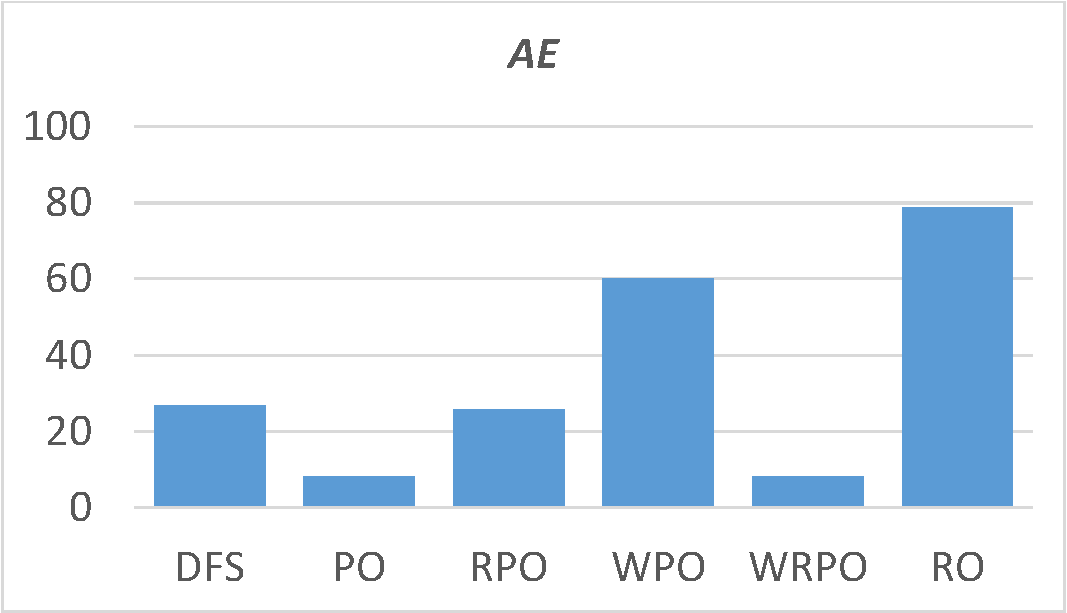
\includegraphics[width=0.32\linewidth]{ecoop-figures/ae-crop.pdf}
%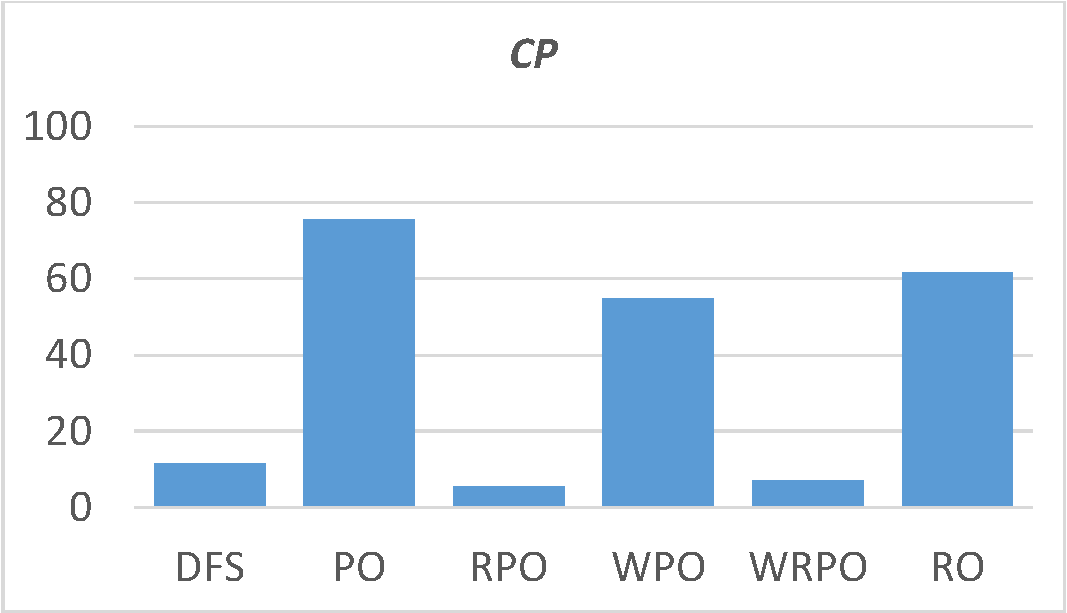
\includegraphics[width=0.32\linewidth]{ecoop-figures/cp-crop.pdf}
%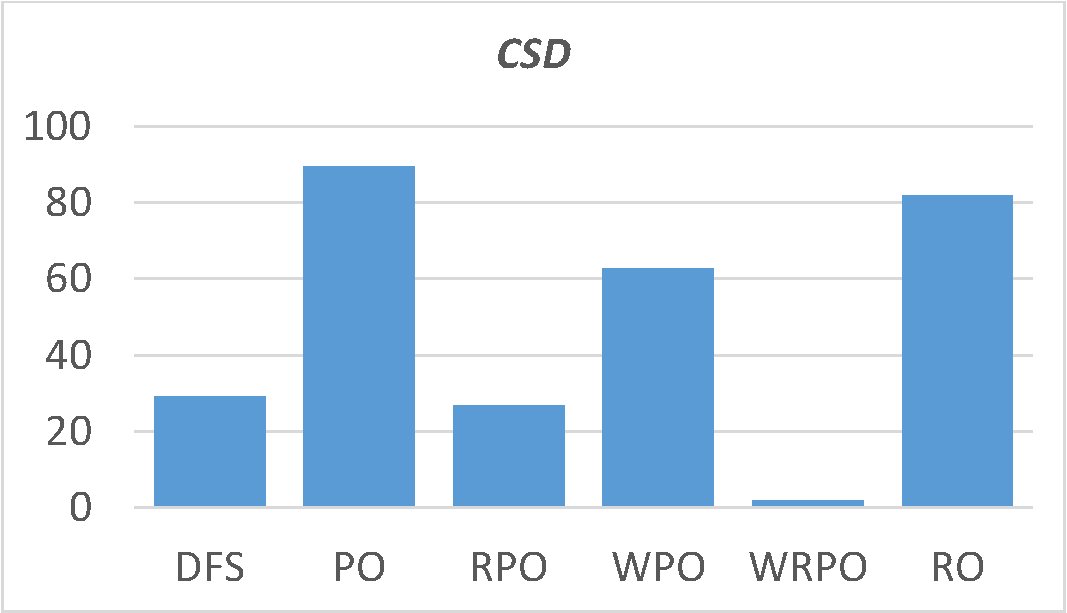
\includegraphics[width=0.32\linewidth]{ecoop-figures/csd-crop.pdf}
%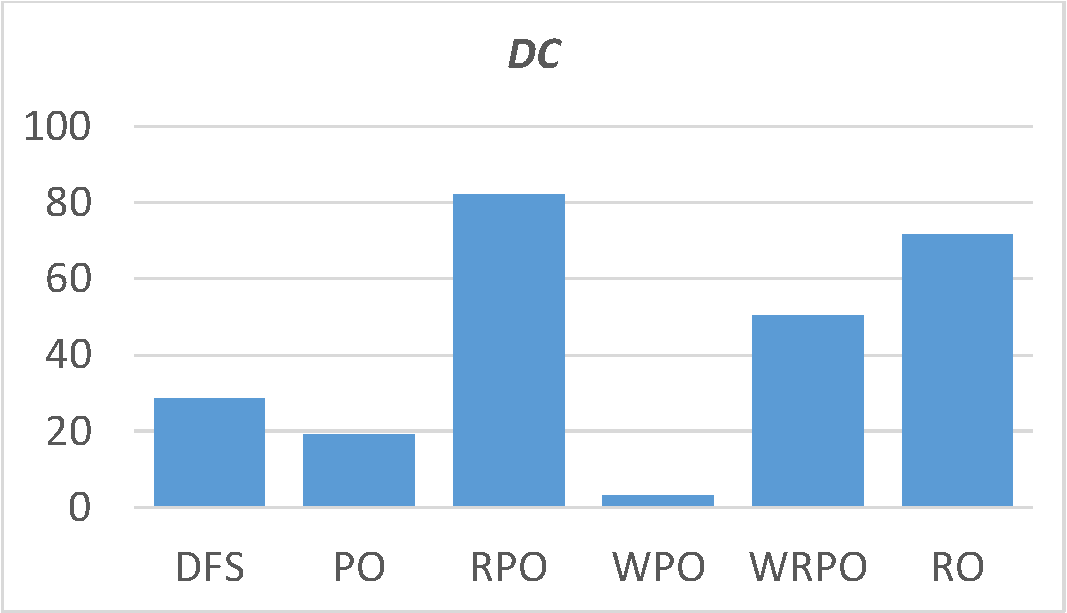
\includegraphics[width=0.32\linewidth]{ecoop-figures/dc-crop.pdf}
%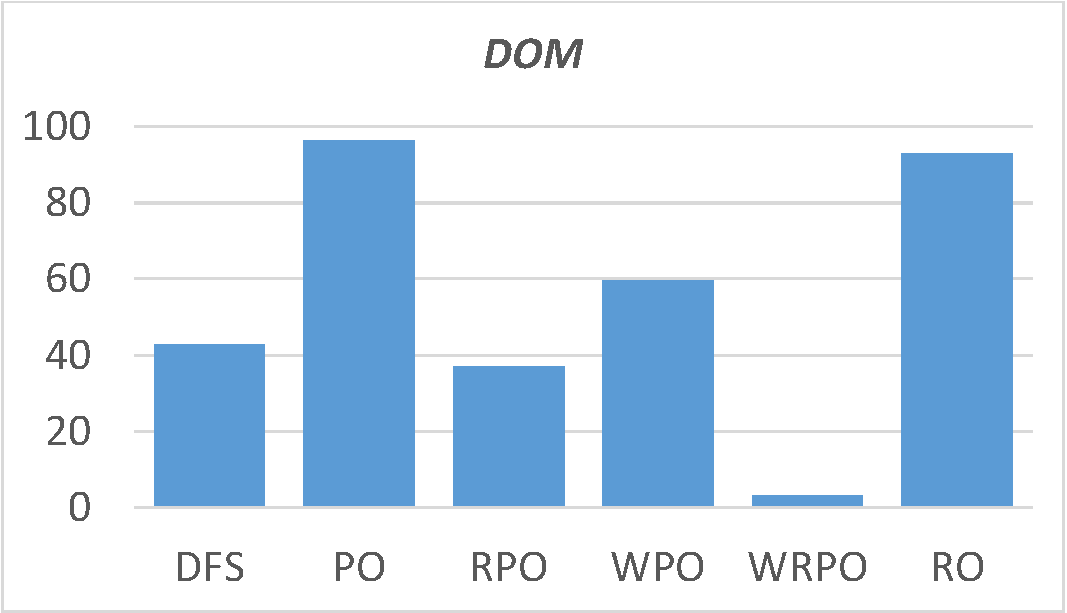
\includegraphics[width=0.32\linewidth]{ecoop-figures/dom-crop.pdf}
%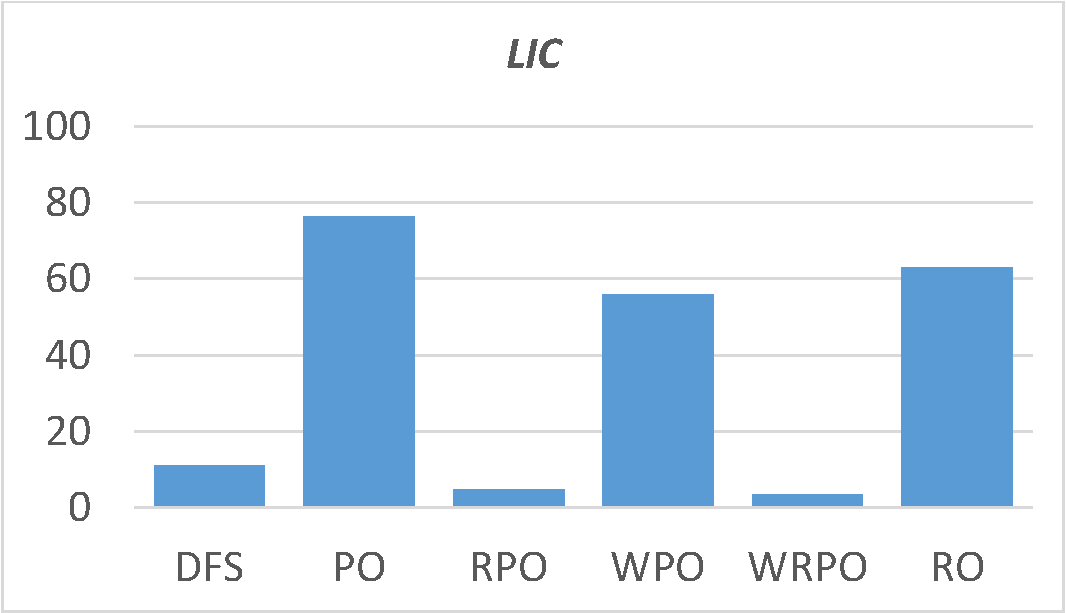
\includegraphics[width=0.32\linewidth]{ecoop-figures/lic-crop.pdf}
%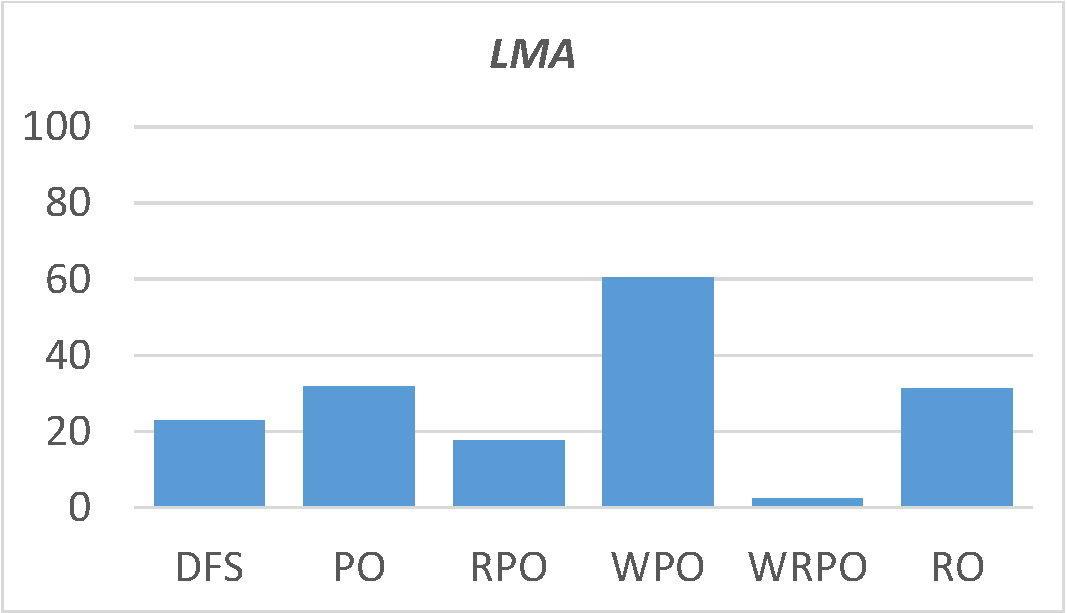
\includegraphics[width=0.32\linewidth]{ecoop-figures/lma-crop.pdf}
%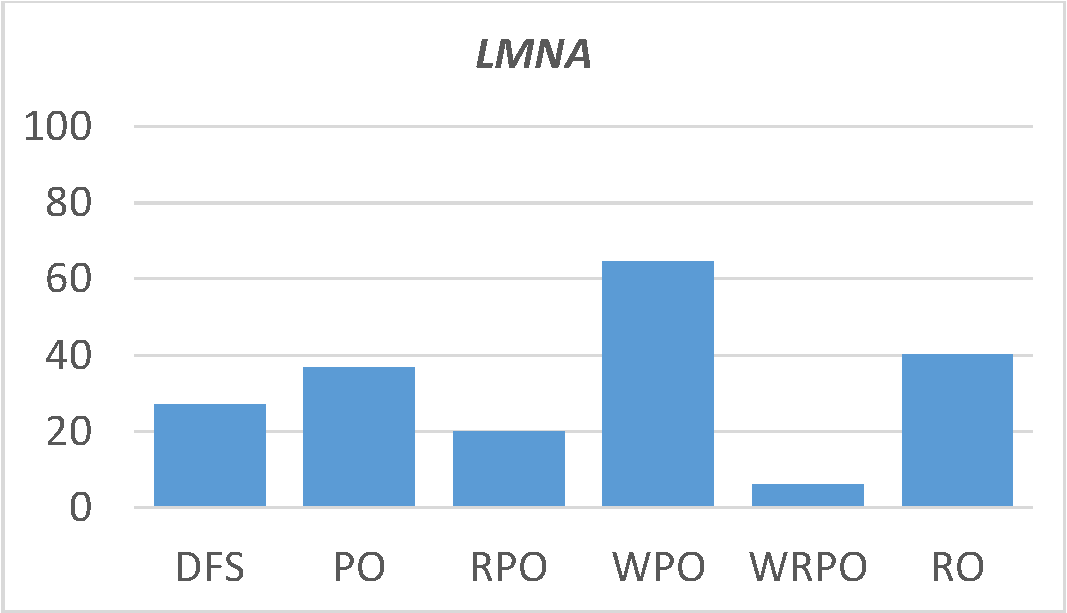
\includegraphics[width=0.32\linewidth]{ecoop-figures/lmna-crop.pdf}
%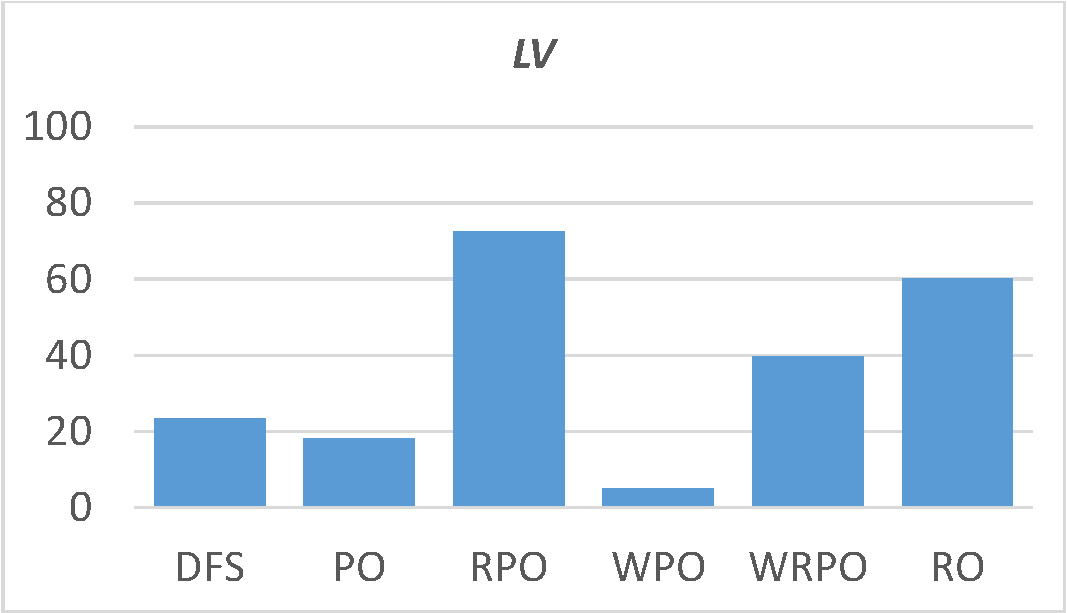
\includegraphics[width=0.32\linewidth]{ecoop-figures/lv-crop.pdf}
%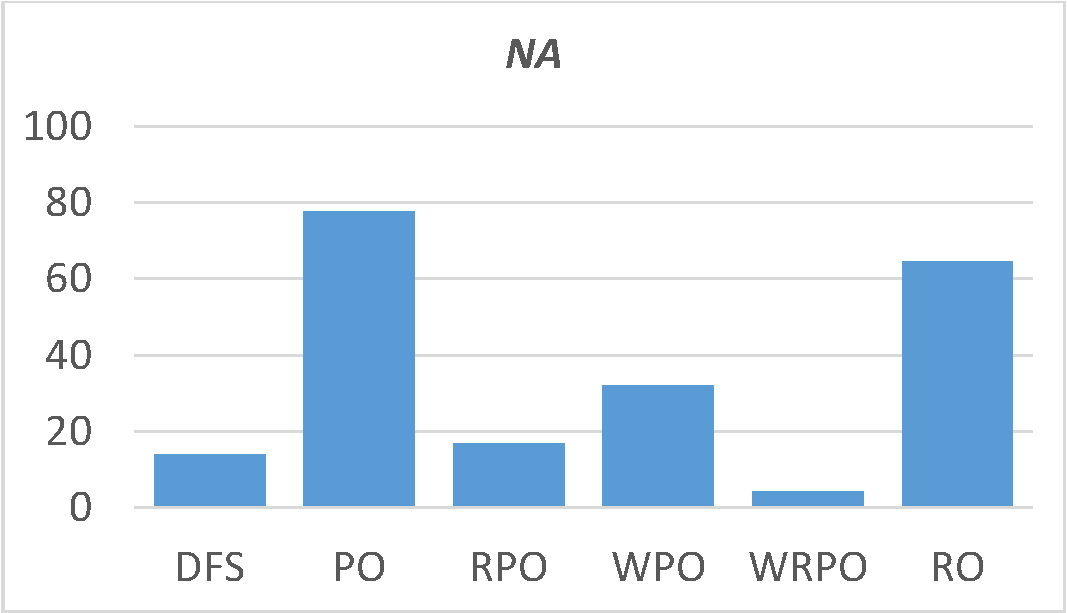
\includegraphics[width=0.32\linewidth]{ecoop-figures/na-crop.pdf}
%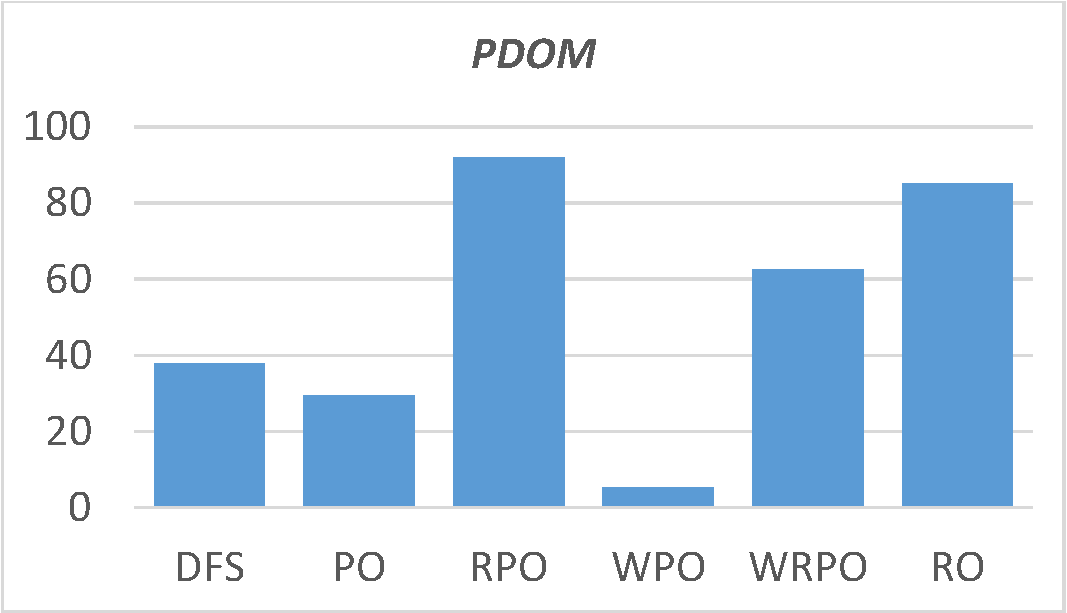
\includegraphics[width=0.32\linewidth]{ecoop-figures/pdom-crop.pdf}
%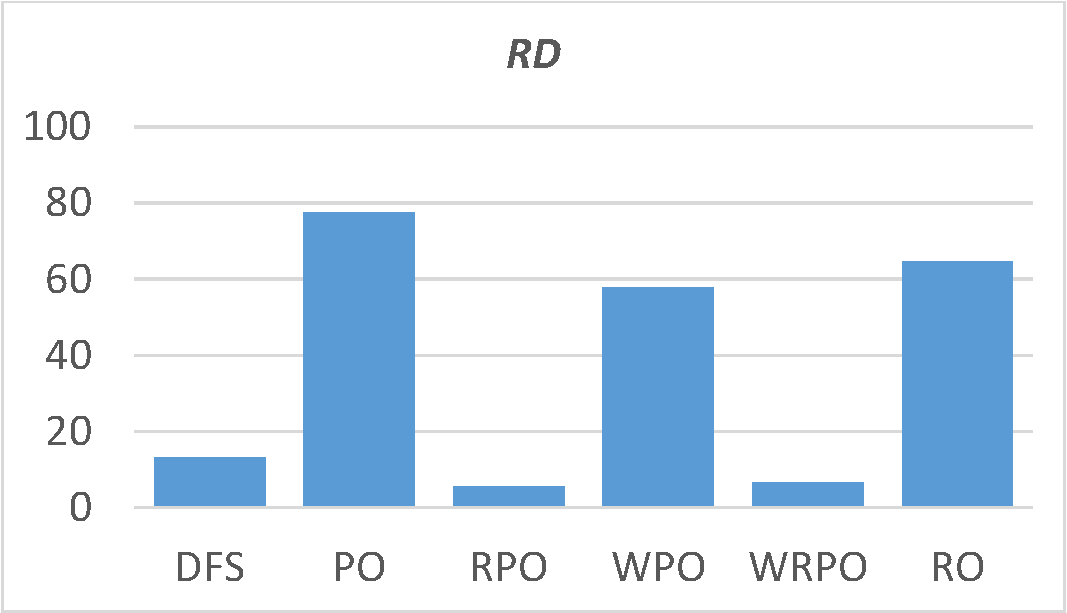
\includegraphics[width=0.32\linewidth]{ecoop-figures/rd-crop.pdf}
%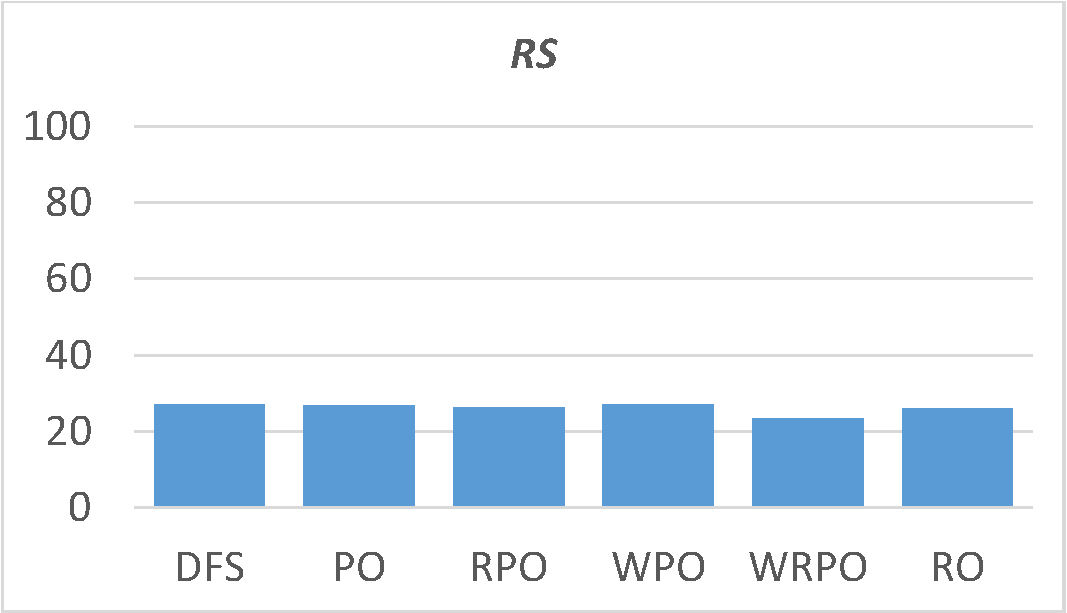
\includegraphics[width=0.32\linewidth]{ecoop-figures/rs-crop.pdf}
%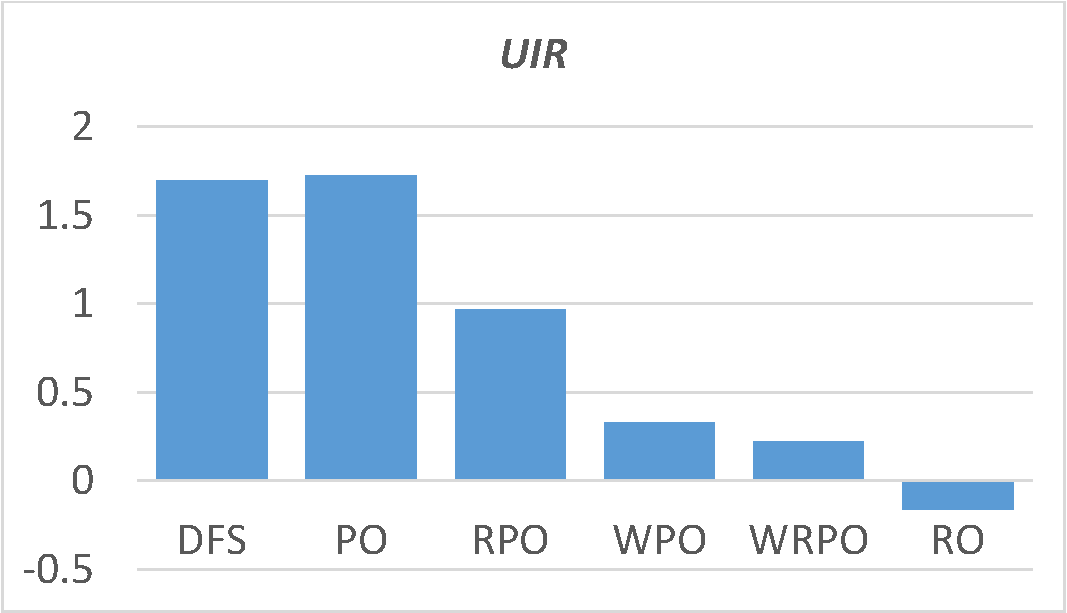
\includegraphics[width=0.32\linewidth]{ecoop-figures/uir-crop.pdf}
%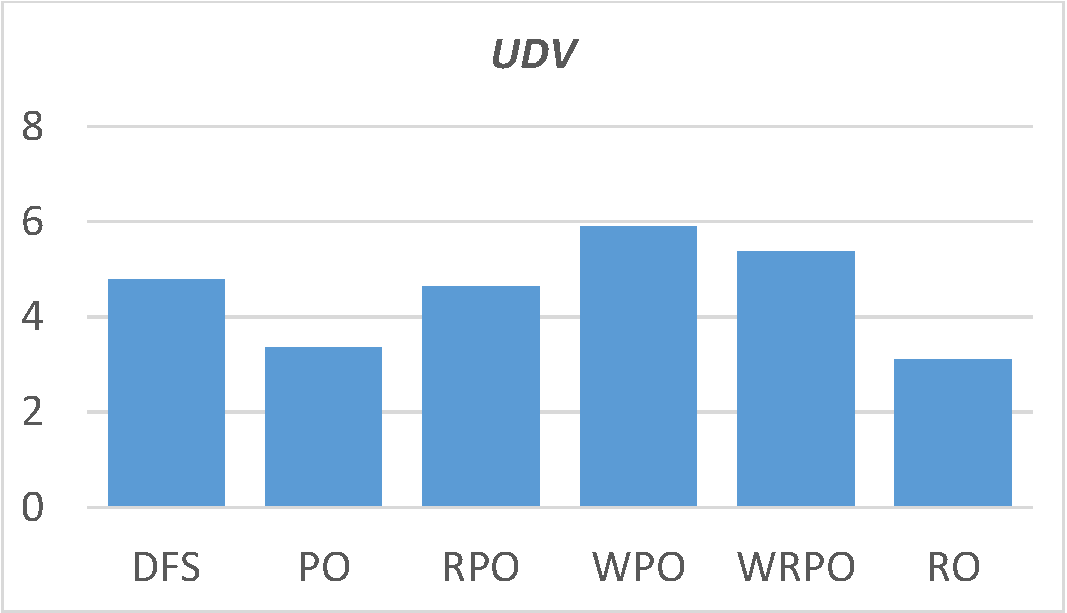
\includegraphics[width=0.32\linewidth]{ecoop-figures/udv-crop.pdf}
%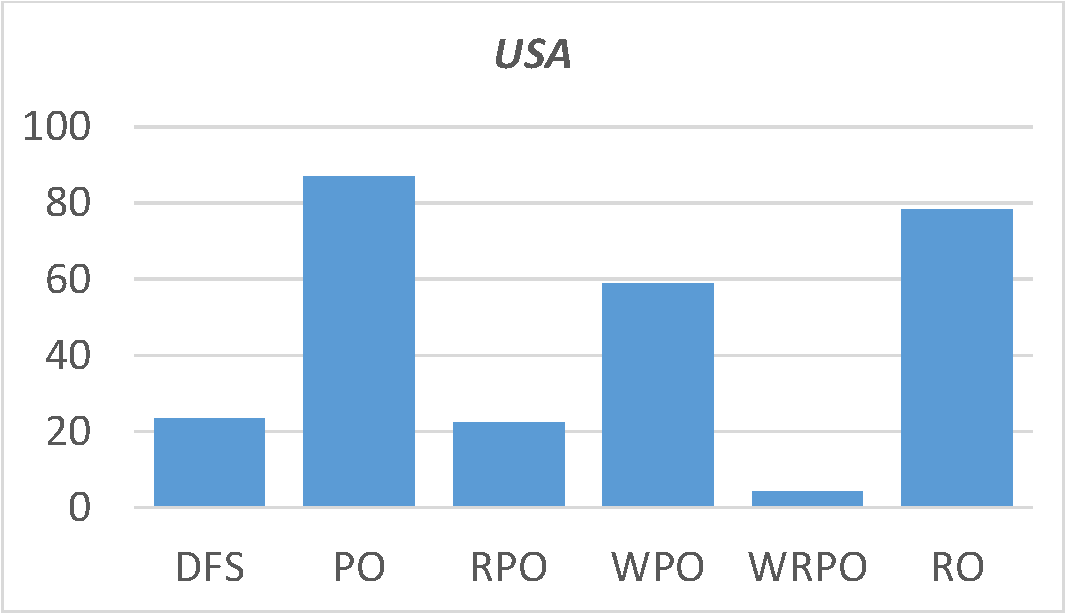
\includegraphics[width=0.32\linewidth]{ecoop-figures/usa-crop.pdf}
%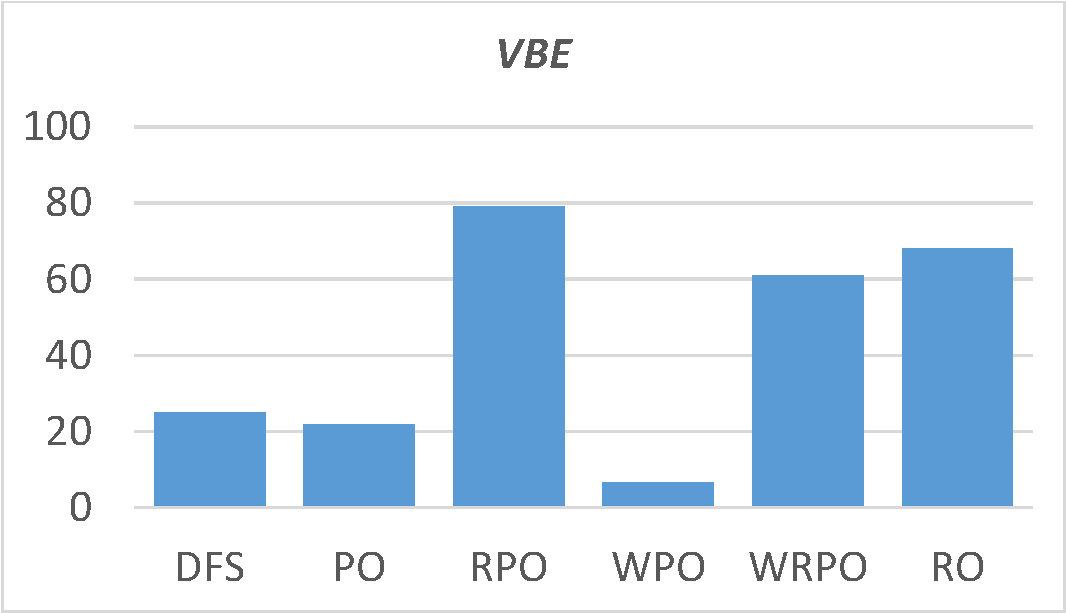
\includegraphics[width=0.32\linewidth]{ecoop-figures/vbe-crop.pdf}
%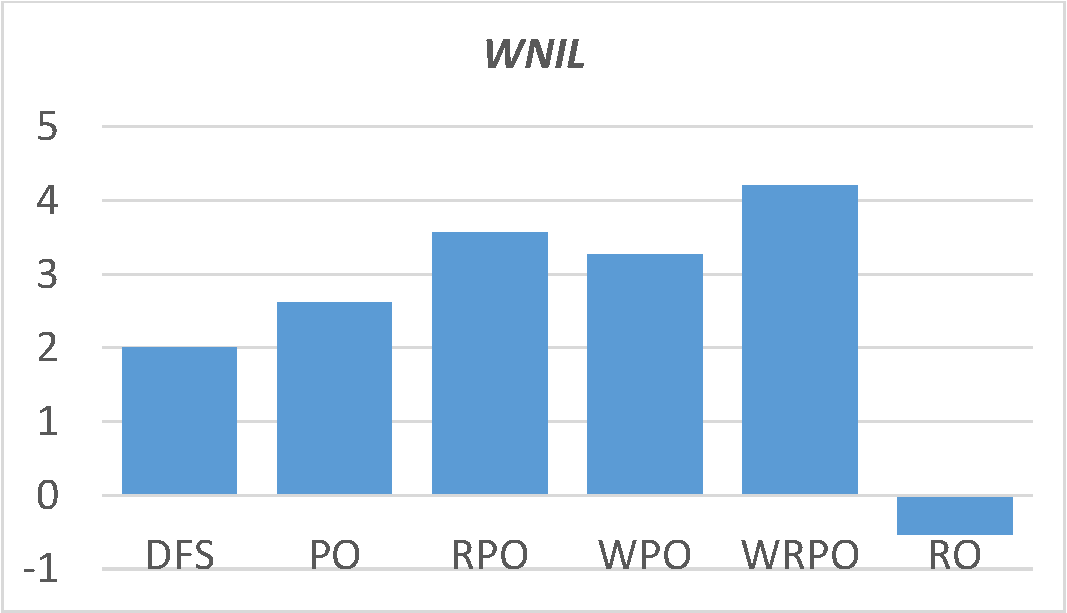
\includegraphics[width=0.32\linewidth]{ecoop-figures/wnil-crop.pdf}\newline
%\textbf{c) \textit{Overall}}\\
%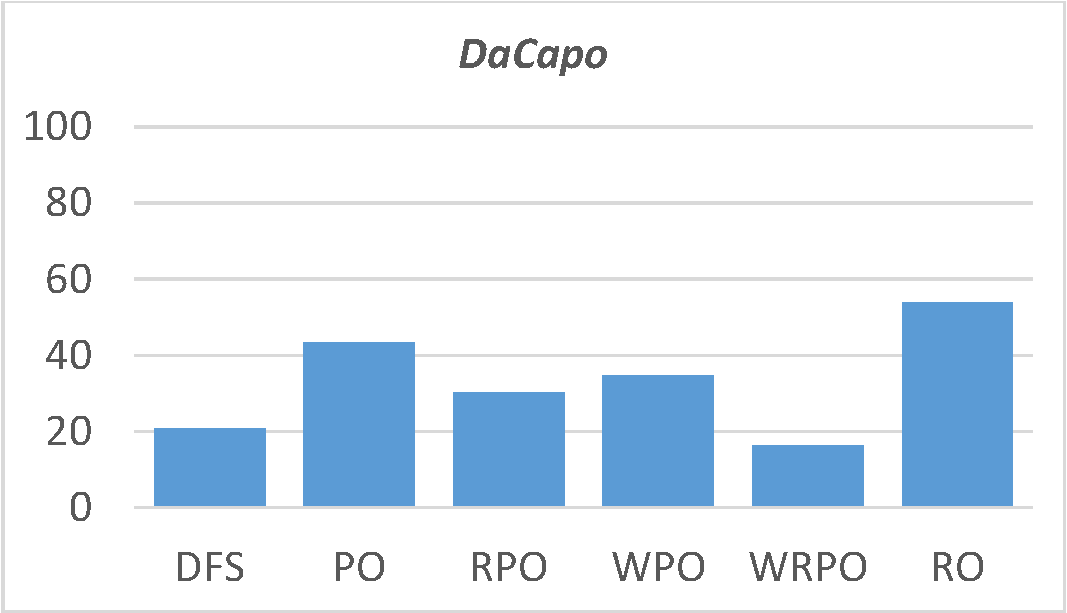
\includegraphics[width=0.32\linewidth]{ecoop-figures/dacapo-overall-crop.pdf}
  %\caption[Percentage reduction in execution time of hybrid approach over other candidate traversals on \textit{DaCapo} (Sequential mode) and \textit{SourceForge} (Cluster mode).]
%{Percentage reduction in execution time of hybrid approach over other candidate traversals on \textit{DaCapo} (Sequential mode) and \textit{SourceForge} (Cluster mode).
%\label{fig:dacapo-singlemachine-time-percentage}}
%\end{figure*}

%\begin{figure*}[ht!]
%\centering
%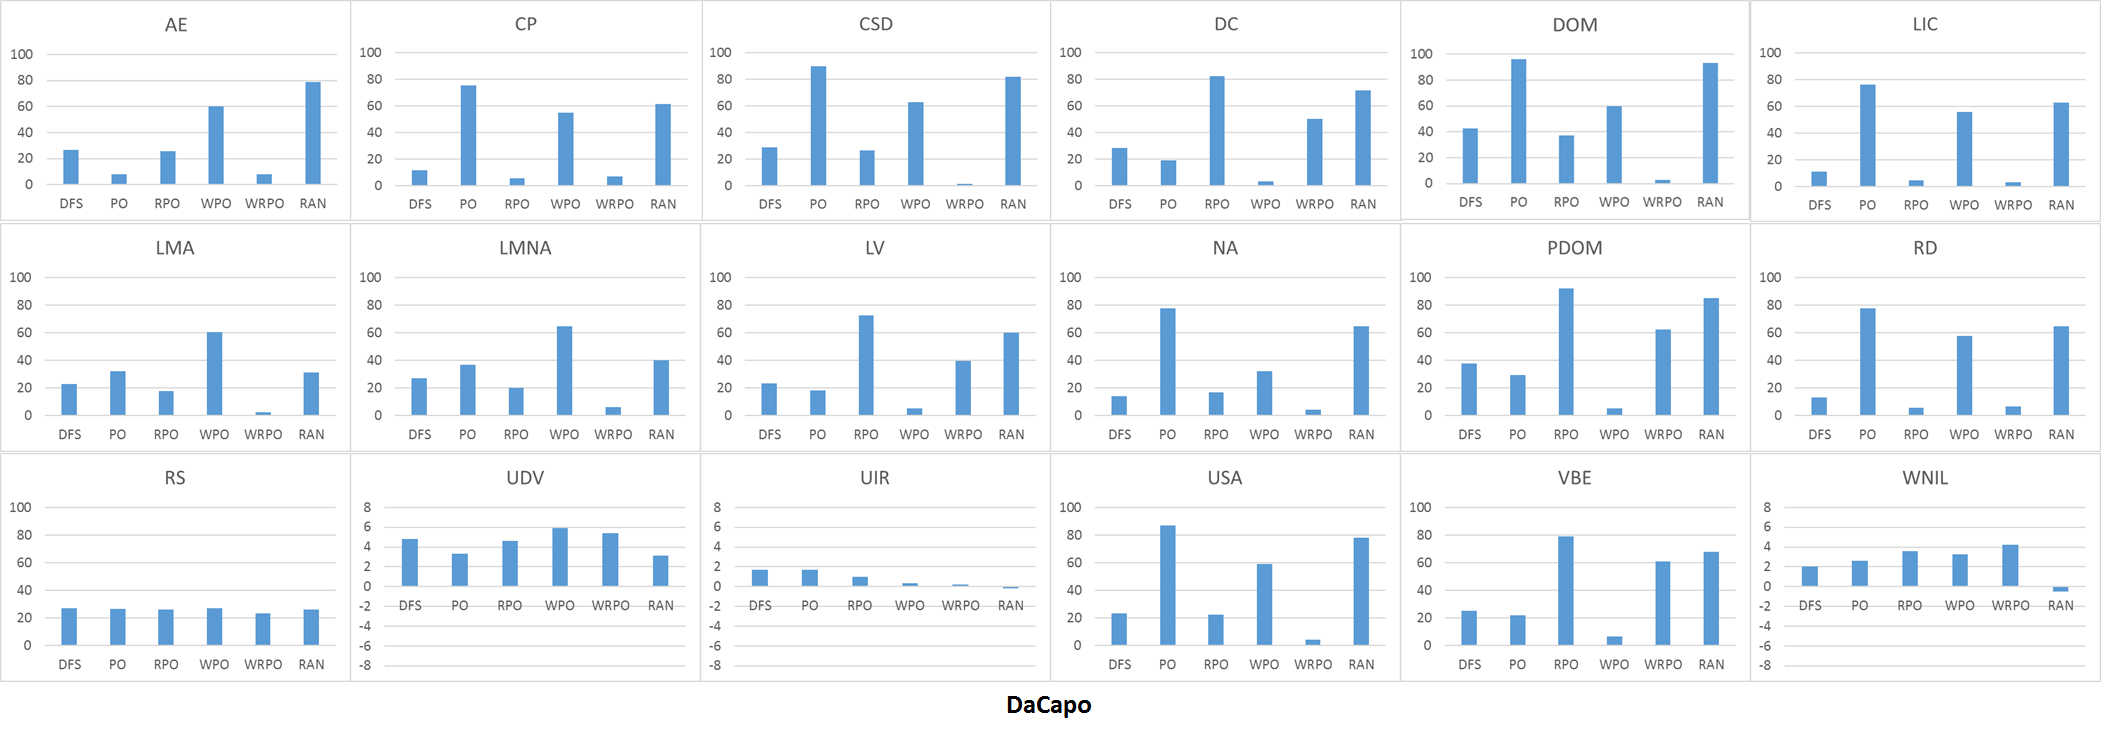
\includegraphics[width=\textwidth]{ecoop-figures/dacapo-seq-reduction.png}
%  \caption[Percentage reduction in execution time of hybrid approach over other candidate traversals on \textit{DaCapo} (Sequential mode), \textit{DaCapo} (Cluster mode), \textit{SourceForge} (Cluster mode).]
%{Percentage reduction in execution time of hybrid approach over other candidate traversals on \textit{DaCapo} (Sequential mode), \textit{DaCapo} (Cluster mode), \textit{SourceForge} (Cluster mode).
%\label{fig:dacapo-singlemachine-time-percentage}}
%\end{figure*}

\begin{figure*}[t]%
\centering
\scriptsize
\subfloat[Time reduction for each analysis.] {
\begin{tabular}{lrrrrrr|rrrrrr}
\toprule
\multicolumn{1}{l}{Analysis} & \multicolumn{6}{c|}{DaCapo}                    & \multicolumn{6}{c}{GitHub} \\
\cmidrule(lr){2-7} \cmidrule(lr){8-13}
      & DFS   & PO    & RPO   & WPO   & WRPO  & ANY    & DFS   & PO    & RPO   & WPO   & WRPO  & ANY \\
\midrule
\multicolumn{1}{l}{CP} & \cellcolor{lightblack}17\%  & \cellcolor{lightgreen}83\%  &  \cellcolor{lightblue}9\%   & \cellcolor{lightgreen}66\%  &  \cellcolor{lightblack}11\%   & \cellcolor{lightgreen}72\%  & \cellcolor{lightblack}17\%  & \cellcolor{lightgreen}88\%  &  \cellcolor{lightblack}12\%   & \cellcolor{lightgreen}80\%  &  \cellcolor{lightblue}5\%   & \cellcolor{lightgreen}82\% \\
\multicolumn{1}{l}{CSD} & \cellcolor{lightblack}41\%  & \cellcolor{lightgreen}93\%  & \cellcolor{lightblack}39\%  & \cellcolor{lightgreen}74\%  &  \cellcolor{lightblue}4\%   & \cellcolor{lightgreen}89\%  & \cellcolor{lightblack}31\%  & --  & \cellcolor{lightblack}24\%  & --  &  \cellcolor{lightblack}12\%   & -- \\
\multicolumn{1}{l}{DC} & \cellcolor{lightblack}41\%  & \cellcolor{lightblack}30\%  & \cellcolor{lightgreen}89\%  &  \cellcolor{lightblue}7\%   & \cellcolor{lightgreen}64\%  & \cellcolor{lightgreen}81\%  & \cellcolor{lightblack}25\%  & \cellcolor{lightblack}22\%  & --  &  \cellcolor{lightblue}7\%   & --  & -- \\
\multicolumn{1}{l}{LIC} & \cellcolor{lightblack}17\%  & \cellcolor{lightgreen}84\%  &  \cellcolor{lightblue}8\%   & \cellcolor{lightgreen}67\%  &  \cellcolor{lightblue}7\%   & \cellcolor{lightgreen}73\%  & \cellcolor{lightblack}19\%  & \cellcolor{lightgreen}89\%  &  \cellcolor{lightblack}15\%   & \cellcolor{lightgreen}81\%  &  \cellcolor{lightblack}19\%   & \cellcolor{lightgreen}88\% \\
\multicolumn{1}{l}{USA} & \cellcolor{lightblack}36\%  & \cellcolor{lightgreen}92\%  & \cellcolor{lightblack}34\%  & \cellcolor{lightgreen}72\%  &  \cellcolor{lightblue}9\%   & \cellcolor{lightgreen}87\%  & \cellcolor{lightblack}22\%  & --  & \cellcolor{lightblack}17\%  & --  &  \cellcolor{lightblue}9\%   & -- \\
\multicolumn{1}{l}{VFR} & \cellcolor{lightblack}20\%  & \cellcolor{lightblack}41\%  & \cellcolor{lightblack}18\%  & \cellcolor{lightgreen}51\%  & \cellcolor{lightblack}15\%  & \cellcolor{lightgreen}62\%  & \cellcolor{lightblack}15\%  & \cellcolor{lightblack}40\%  & \cellcolor{lightblue}10\%  & \cellcolor{lightblack}44\%  & \cellcolor{lightblue}9\%  & \cellcolor{lightgreen}53\% \\
\multicolumn{1}{l}{MWN} & \cellcolor{lightblack}21\%  & \cellcolor{lightblack}35\%  & \cellcolor{lightblack}16\%  & \cellcolor{lightblack}35\%  & \cellcolor{lightblack}22\%  & \cellcolor{lightblack}49\%  & \cellcolor{lightblack}17\%  & \cellcolor{lightblack}31\%  & \cellcolor{lightblack}12\%  & \cellcolor{lightblack}33\%  & \cellcolor{lightblack}11\%  & \cellcolor{lightblack}46\% \\
\multicolumn{1}{l}{AE} & \cellcolor{lightblack}40\%  &  \cellcolor{lightblack}14\%   & \cellcolor{lightblack}39\%  & \cellcolor{lightgreen}73\%  &  \cellcolor{lightblack}14\%   & \cellcolor{lightgreen}87\%  & \cellcolor{lightblack}16\%  &  --   & \cellcolor{lightblack}16\%  & --  &  \cellcolor{lightblack}11\%   & -- \\
\multicolumn{1}{l}{DOM} & \cellcolor{lightblack}54\%  & \cellcolor{lightgreen}97\%  & \cellcolor{lightblack}48\%  & \cellcolor{lightgreen}70\%  &  \cellcolor{lightblue}6\%   & \cellcolor{lightgreen}95\%  & \cellcolor{lightblack}27\%  & --  & \cellcolor{lightblack}32\%  & --  &  \cellcolor{lightblue}6\%   & -- \\
\multicolumn{1}{l}{LMA} & \cellcolor{lightblack}35\%  & \cellcolor{lightblack}46\%  & \cellcolor{lightblack}28\%  & \cellcolor{lightgreen}74\%  &  \cellcolor{lightblue}6\%   & \cellcolor{lightblack}46\%  & \cellcolor{lightblack}22\%  & --  & \cellcolor{lightblack}13\%  & --  &  \cellcolor{lightblue}6\%   & -- \\
\multicolumn{1}{l}{LMNA} & \cellcolor{lightblack}29\%  & \cellcolor{lightblack}39\%  & \cellcolor{lightblack}22\%  & \cellcolor{lightgreen}68\%  &  \cellcolor{lightblue}9\%   & \cellcolor{lightblack}41\%  & \cellcolor{lightblack}21\%  & --  & \cellcolor{lightblack}15\%  & --  &  \cellcolor{lightblue}7\%   & -- \\
\multicolumn{1}{l}{LV} & \cellcolor{lightblack}38\%  & \cellcolor{lightblack}30\%  & \cellcolor{lightgreen}84\%  &  \cellcolor{lightblack}11\%   & \cellcolor{lightblack}56\%  & \cellcolor{lightgreen}75\%  & \cellcolor{lightblack}25\%  & \cellcolor{lightblack}21\%  & \cellcolor{lightgreen}68\%  &  \cellcolor{lightblack}11\%   & \cellcolor{lightblack}69\%  & \cellcolor{lightgreen}80\% \\
\multicolumn{1}{l}{NA} & \cellcolor{lightblack}26\%  & \cellcolor{lightgreen}88\%  & \cellcolor{lightblack}30\%  & \cellcolor{lightblack}50\%  &  \cellcolor{lightblue}10\%   & \cellcolor{lightgreen}80\%  & \cellcolor{lightblack}13\%  & \cellcolor{lightgreen}87\%  & \cellcolor{lightblack}12\%  & \cellcolor{lightgreen}71\%  &  \cellcolor{lightblue}10\%   & \cellcolor{lightgreen}85\% \\
\multicolumn{1}{l}{PDOM} & \cellcolor{lightblack}51\%  & \cellcolor{lightblack}41\%  & \cellcolor{lightgreen}95\%  &  \cellcolor{lightblue}10\%   & \cellcolor{lightgreen}72\%  & \cellcolor{lightgreen}95\%  & \cellcolor{lightblack}24\%  & \cellcolor{lightblack}20\%  & --  &  \cellcolor{lightblack}24\%   & --  & -- \\
\multicolumn{1}{l}{RD} & \cellcolor{lightblack}15\%  & \cellcolor{lightgreen}80\%  &  \cellcolor{lightblue}7\%   & \cellcolor{lightgreen}62\%  &  \cellcolor{lightblue}9\%   & \cellcolor{lightgreen}68\%  & \cellcolor{lightblack}19\%  & \cellcolor{lightgreen}91\%  &  \cellcolor{lightblue}10\%   & \cellcolor{lightgreen}79\%  &  \cellcolor{lightblue}5\%   & \cellcolor{lightgreen}86\% \\
\multicolumn{1}{l}{RS} & \cellcolor{lightblack}31\%  & \cellcolor{lightblack}31\%  & \cellcolor{lightblack}30\%  & \cellcolor{lightblack}31\%  & \cellcolor{lightblack}28\%  & \cellcolor{lightblack}30\%  & \cellcolor{lightblack}16\%  & \cellcolor{lightblack}40\%  & \cellcolor{lightblue}9\%  & \cellcolor{lightblack}31\%  & \cellcolor{lightblue}7\%  & \cellcolor{lightblack}49\% \\
\multicolumn{1}{l}{VBE} & \cellcolor{lightblack}40\%  & \cellcolor{lightblack}36\%  & \cellcolor{lightgreen}88\%  &  \cellcolor{lightblack}13\%   & \cellcolor{lightgreen}76\%  & \cellcolor{lightgreen}81\%  & \cellcolor{lightblack}28\%  & \cellcolor{lightblack}24\%  & --  &  \cellcolor{lightblue}10\%   & --  & -- \\
\multicolumn{1}{l}{SS} & \cellcolor{lightblack}26\%  & \cellcolor{lightblack}39\%  & \cellcolor{lightblack}22\%  & \cellcolor{lightblack}37\%  & \cellcolor{lightblack}25\%  & \cellcolor{lightgreen}57\%  & \cellcolor{lightblack}20\%  & \cellcolor{lightblack}35\%  & \cellcolor{lightblack}13\%  & \cellcolor{lightblack}34\%  & \cellcolor{lightblue}10\%  & \cellcolor{lightgreen}50\% \\
\multicolumn{1}{l}{UDV} &  \cellcolor{lightblue}6\%   &  \cellcolor{lightblue}5\%   &  \cellcolor{lightblue}6\%   &  \cellcolor{lightblue}10\%   &  \cellcolor{lightblue}9\%   &  \cellcolor{lightblue}3\%   &  \cellcolor{lightblue}3\%   &  \cellcolor{lightblue}4\%   &  \cellcolor{lightblue}2\%   &  \cellcolor{lightblue}7\%   &  \cellcolor{lightblue}6\%   &  \cellcolor{lightblue}0\% \\
\multicolumn{1}{l}{UIR} &  \cellcolor{lightblue}2\%   &  \cellcolor{lightblue}2\%   &  \cellcolor{lightblue}1\%   & \cellcolor{lightblue}3\%   & \cellcolor{lightblue}3\%   & \cellcolor{lightblue}0\%   &  \cellcolor{lightblue}2\%   &  \cellcolor{lightblue}5\%   &  \cellcolor{lightblue}4\%   & \cellcolor{lightblue}7\%   & \cellcolor{lightblue}7\%   & \cellcolor{lightblue}0\% \\
\multicolumn{1}{l}{WNIL} &  \cellcolor{lightblue}3\%   &  \cellcolor{lightblue}4\%   &  \cellcolor{lightblue}5\%   &  \cellcolor{lightblue}6\%   &  \cellcolor{lightblue}8\%   & \cellcolor{lightblue}2\%  &  \cellcolor{lightblue}3\%   &  \cellcolor{lightblue}6\%   &  \cellcolor{lightblue}5\%   &  \cellcolor{lightblue}5\%   &  \cellcolor{lightblue}6\%   & \cellcolor{lightblue}0\% \\
\midrule
\multicolumn{1}{l}{Overall} &  \cellcolor{lightblack}31\%   &  \cellcolor{lightgreen}83\%   &  \cellcolor{lightgreen}70\%   &  \cellcolor{lightblack}55\%   &  \cellcolor{lightblack}35\%   &  \cellcolor{lightgreen}81\%   &  --   &  --  &  --   &  --   &  --  &  -- \\
\bottomrule
\end{tabular}%
\label{tab:reduction-analyses}
}\\
\subfloat[Overall reduction over analysis properties.] {
\setlength{\tabcolsep}{3.5pt}
\begin{tabular}{lrrrrrr}
\toprule
\multicolumn{1}{l}{Property} & \multicolumn{6}{c}{DaCapo}   \\
\cmidrule(lr){2-7}
      & DFS   & PO    & RPO   & WPO   & WRPO  & ANY   \\
\midrule
\multicolumn{1}{l}{Data-flow} & \cellcolor{lightblack}32\%  & \cellcolor{lightgreen}84\%  &  \cellcolor{lightgreen}72\%   & \cellcolor{lightgreen}57\%  &  \cellcolor{lightblack}36\%   & \cellcolor{lightgreen}83\% \\
\multicolumn{1}{l}{$\neg$Data-flow} & \cellcolor{lightblue}4\%  & \cellcolor{lightblue}4\%  & \cellcolor{lightblue}4\%  & \cellcolor{lightblue}6\%  &  \cellcolor{lightblue}6\%   & \cellcolor{lightblue}2\% \\
\bottomrule
\end{tabular}%
\label{tab:reduction-analysis-properties}
}
\subfloat[Overall reduction over graph properties.] {
\setlength{\tabcolsep}{3.5pt}
\begin{tabular}{lrrrrrr}
\toprule
\multicolumn{1}{l}{Property} & \multicolumn{6}{c}{DaCapo} \\
\cmidrule(lr){2-7} 
      & DFS   & PO    & RPO   & WPO   & WRPO  & ANY   \\
\midrule
\multicolumn{1}{l}{Sequential} & \cellcolor{lightblack}20\%  & \cellcolor{lightgreen}74\%  &  \cellcolor{lightgreen}63\%   & \cellcolor{lightgreen}55\%  &  \cellcolor{lightblack}28\%   & \cellcolor{lightgreen}72\%  \\
\multicolumn{1}{l}{Branch} & \cellcolor{lightblack}31\%  & \cellcolor{lightgreen}81\%  & \cellcolor{lightgreen}66\%  & \cellcolor{lightgreen}58\%  &  \cellcolor{lightblack}40\%   & \cellcolor{lightgreen}92\% \\
\multicolumn{1}{l}{Loop} & \cellcolor{lightgreen}53\%  & \cellcolor{lightgreen}88\%  & \cellcolor{lightgreen}75\%  &  \cellcolor{lightgreen}62\%   & \cellcolor{lightblack}37\%  & \cellcolor{lightgreen}95\% \\
\bottomrule
\end{tabular}%
\label{tab:reduction-graph-properties}
}
\caption{Reduction in running times.}
\label{fig:reduction}
\end{figure*}


To evaluate the efficiency in running time of the hybrid approach over other 
traversal strategies, we ran the 21 analyses on DaCapo and GitHub 
datasets using hybrid approach and other candidate traversals. When comparing 
the hybrid approach to a standard strategy $S$, we computed the reduction 
rate $R=(T_S-T_H)/T_S$ where $T_S$ and $T_H$ are the running times using the 
standard and the hybrid strategy, respectively. 
%
Some analyses have some worst case traversal strategies which might not be 
feasible to run on dataset at the scale of 162 million graphs as in 
GitHub dataset. For example, using post-order for forward data-flow 
analysis will visit the CFG in the direction which is opposite to the 
natural direction of the analysis and hence takes a lot of time to complete 
the analysis. For such combinations of analyses and traversal strategies, the 
map and the reducer tasks time out in the cluster setting and, thus, we did 
not provide the running times. 
The corresponding cells in \figref{tab:reduction-analyses} are denoted with symbol --.
%And for the same reason that some strategies do not have running time, we have 
%also not calculated hybrid's overall reduction over such strategies.
%
%Analyses on DaCapo were run on sequential mode while those on SourceForge were run on cluster mode. 

The result in \figref{tab:reduction-analyses} shows that the hybrid approach 
helps reduce the running times in almost all cases. The values indicates the 
reduction in running time by adopting hybrid approach compared against the standard strategies. 
%The executions failed on some pairs of analyses and standard traversals due to 
%memory problems which are indicated by the symbol - in the corresponding cells. 
Most of positive reductions are from 10\% (\colorbox{lightblack}{light yellow 
cells}) or even from 50\% (\colorbox{lightgreen}{light green cells}). More 
importantly, the most time-efficient and the worst traversal strategies vary 
across the analyses which supports the need of our hybrid traversal strategy.
%
Over all analyses, the reduction was highest against any order and 
post-order (PO and WPO) strategies. The reduction was lowest against the strategy 
using depth-first search (DFS) and worklist with reverse post-ordering (WRPO). 
When compared with the next best performing traversal strategy for each analysis, hybrid approach reduces the overall execution time by 
about 13 minutes to 72 minutes on GitHub dataset. We do not 
report the overall numbers for GitHub dataset due to the presence of failed 
runs.

\figref{tab:reduction-analysis-properties} shows time reductions for 
different types of analyses. For \textit{data-flow sensitive} ones, the 
reduction rates are high ranging from 32\% to 84\%. 
%The 10\% reduction is when compared 
%to the most popular traversal strategy for the analysis and the 90\% 
%reduction is when compared to the worst performing traversal strategy for the 
%analysis. 
The running time was not improved much for \emph{non data-flow sensitive} 
traversals, which correspond to the last three rows in \figref{tab:reduction-analyses} 
with mostly one digit reductions (\colorbox{lightblue}{light orange 
cells}). 
We actually perform almost as same as Any order traversal 
strategy for analyses in this category. This is because Any order traversal 
strategy is the best strategy for all the CFGs in these analyses. Hybrid 
approach also chooses any order traversal strategy and hence there is no 
scope for performance gain. 

\figref{tab:reduction-graph-properties} shows time reduction for
different \graphprop{} types of input graphs. We can see that
reductions over graphs with loops is highest and those over any graphs
is lowest.

\subsection{Time reduction against hand optimized analysis}
\label{sec:hand-optimized}
%\begin{figure*}[ht!]
%\centering
%\textbf{a) \textit{DaCapo}}\\
%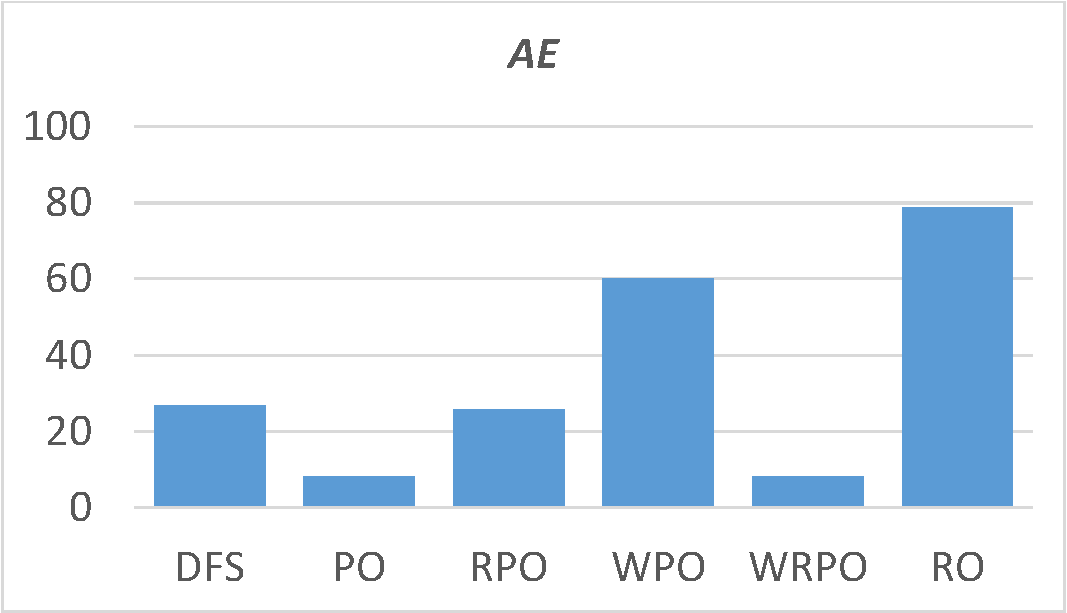
\includegraphics[width=0.32\linewidth]{ecoop-figures/ae-crop.pdf}
%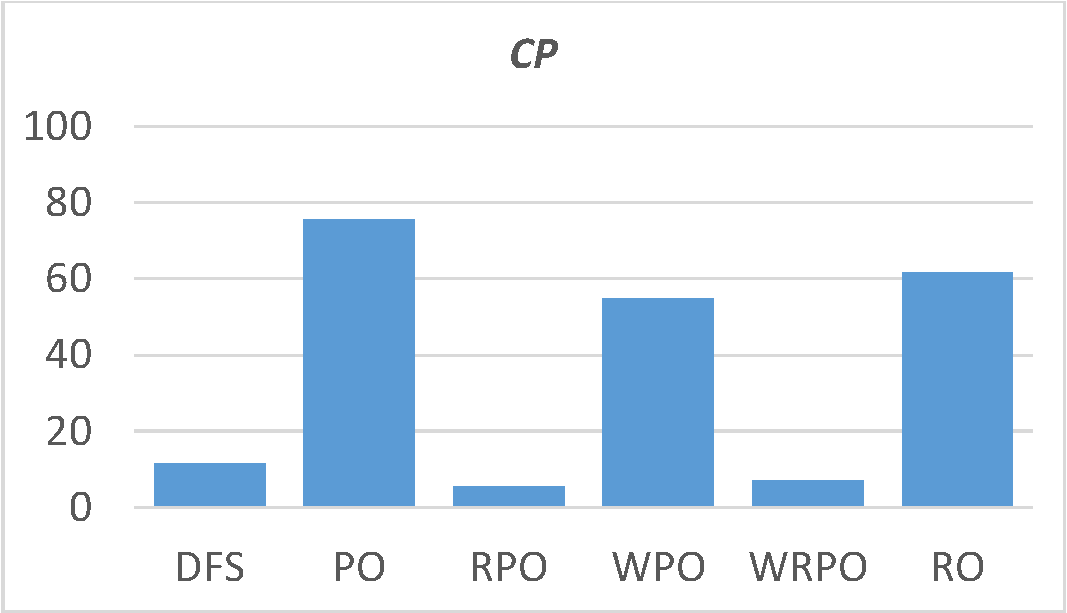
\includegraphics[width=0.32\linewidth]{ecoop-figures/cp-crop.pdf}
%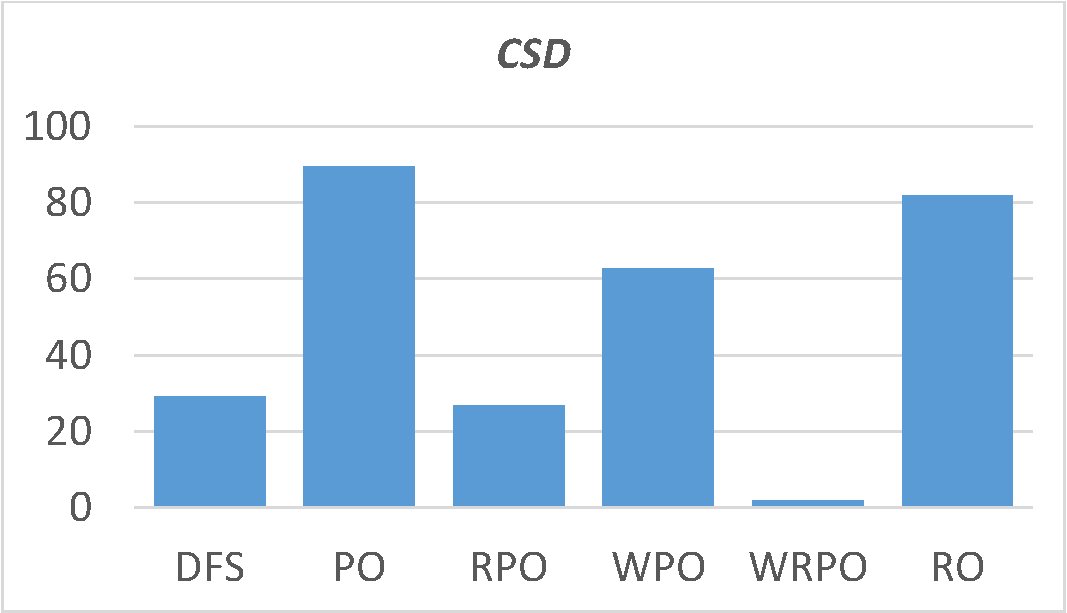
\includegraphics[width=0.32\linewidth]{ecoop-figures/csd-crop.pdf}
%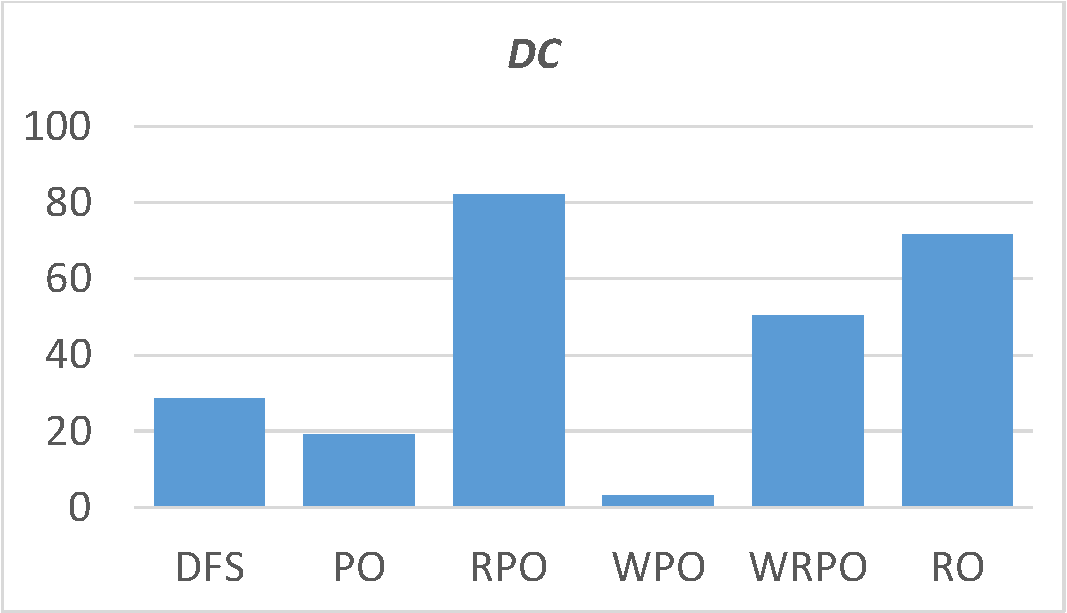
\includegraphics[width=0.32\linewidth]{ecoop-figures/dc-crop.pdf}
%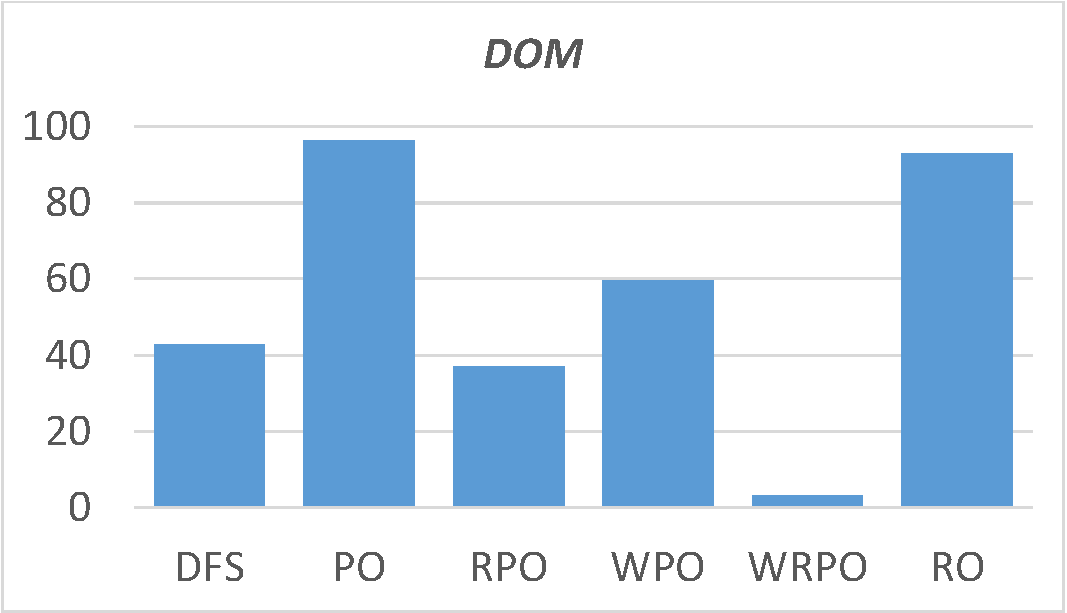
\includegraphics[width=0.32\linewidth]{ecoop-figures/dom-crop.pdf}
%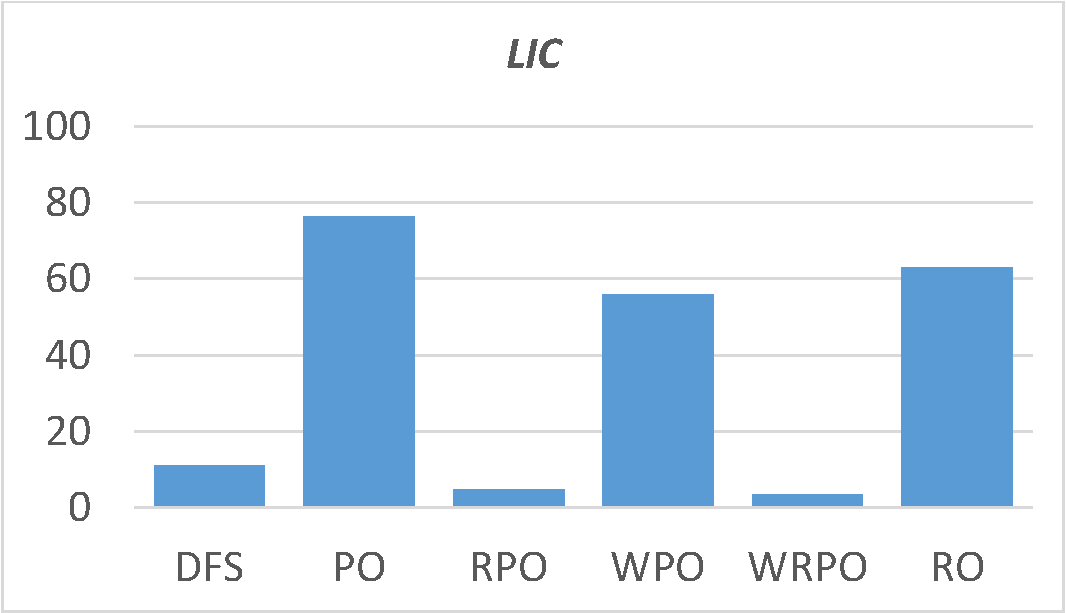
\includegraphics[width=0.32\linewidth]{ecoop-figures/lic-crop.pdf}
%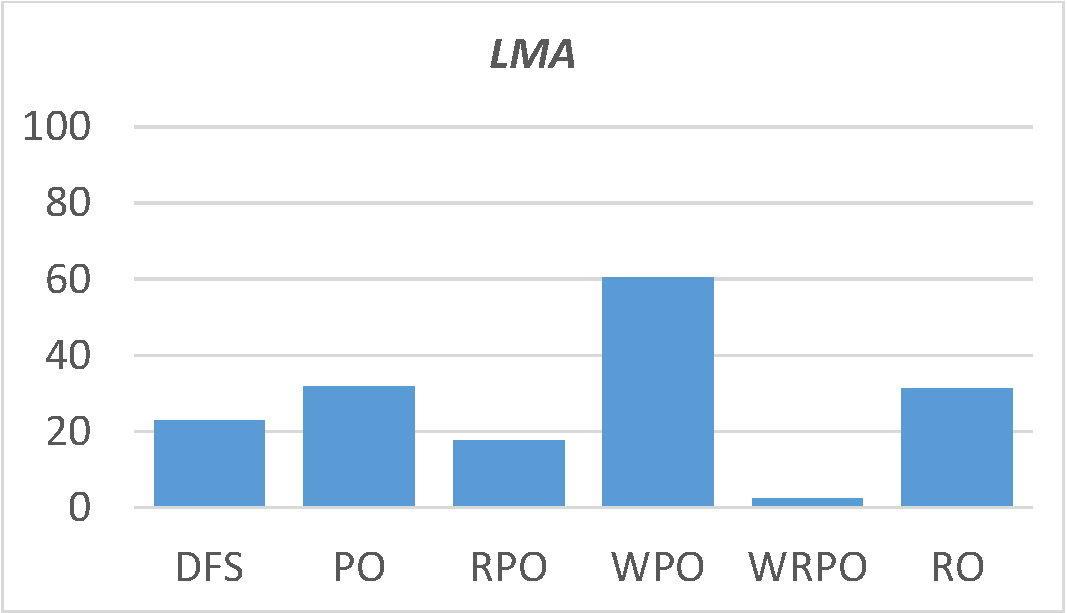
\includegraphics[width=0.32\linewidth]{ecoop-figures/lma-crop.pdf}
%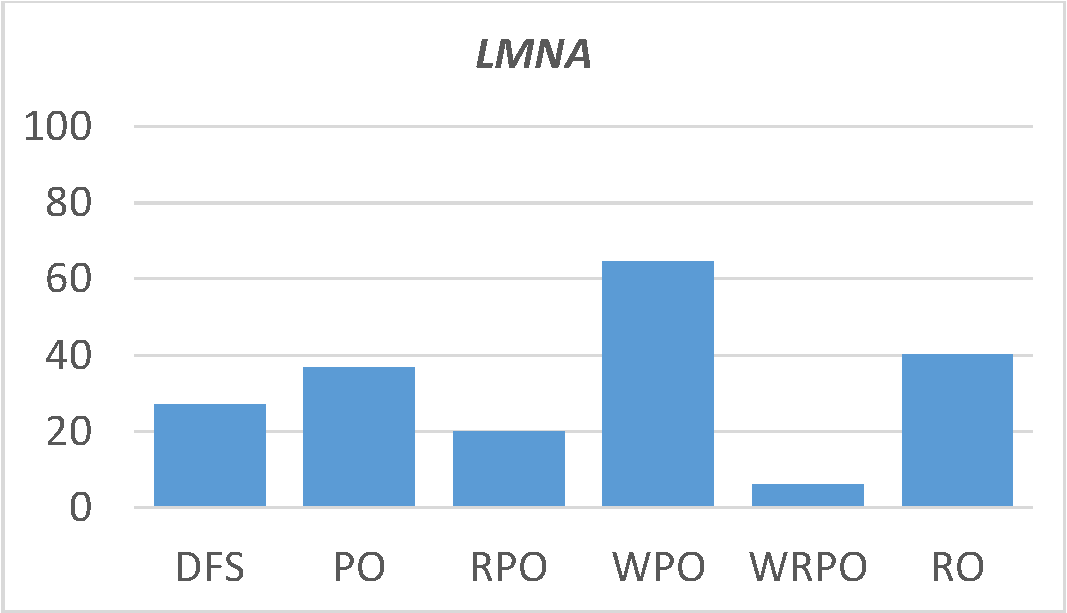
\includegraphics[width=0.32\linewidth]{ecoop-figures/lmna-crop.pdf}
%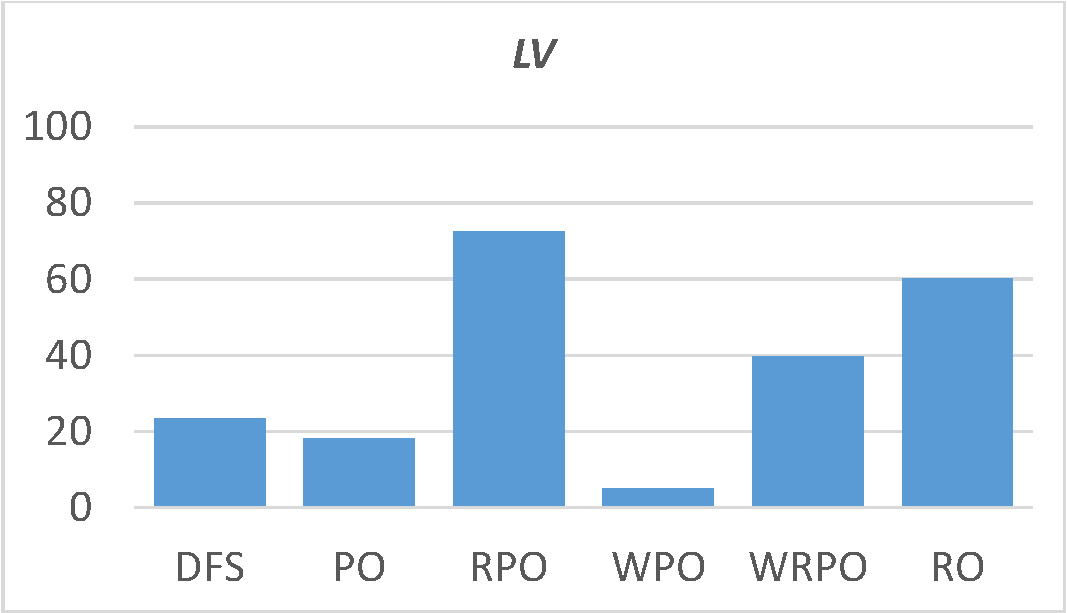
\includegraphics[width=0.32\linewidth]{ecoop-figures/lv-crop.pdf}
%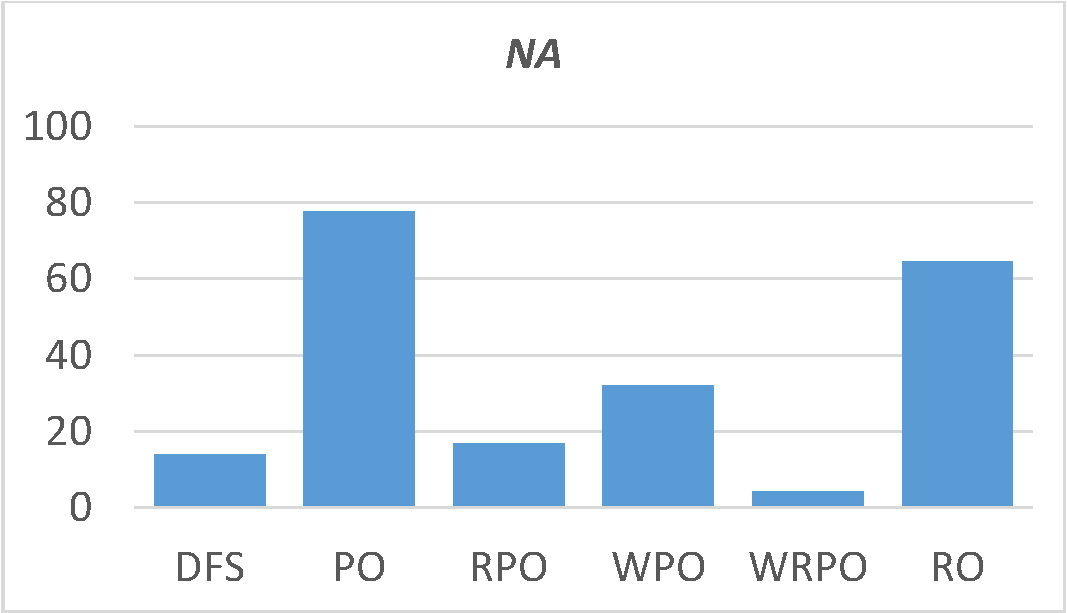
\includegraphics[width=0.32\linewidth]{ecoop-figures/na-crop.pdf}
%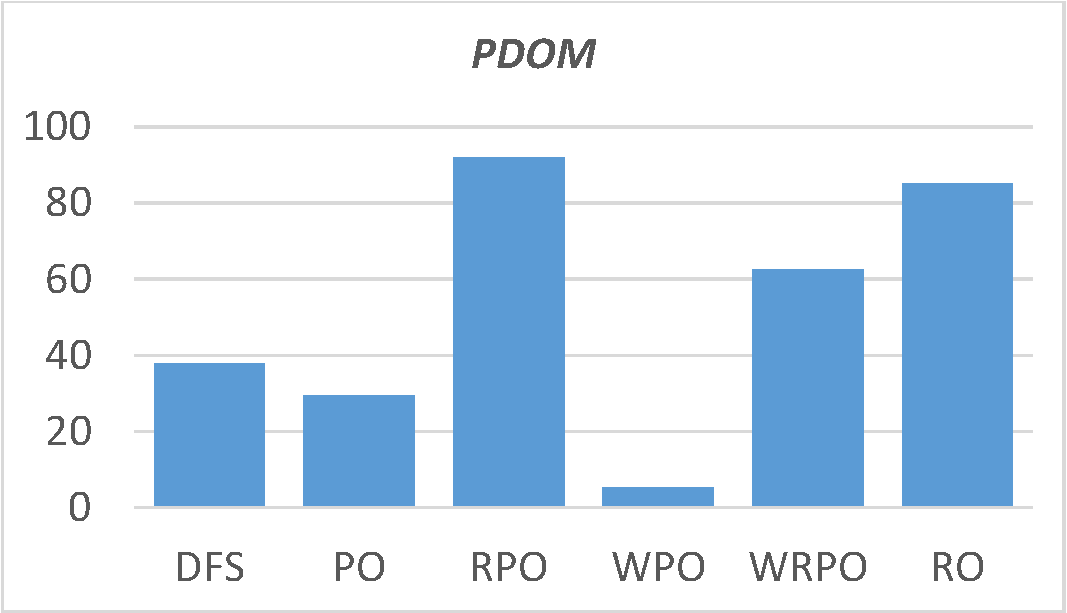
\includegraphics[width=0.32\linewidth]{ecoop-figures/pdom-crop.pdf}
%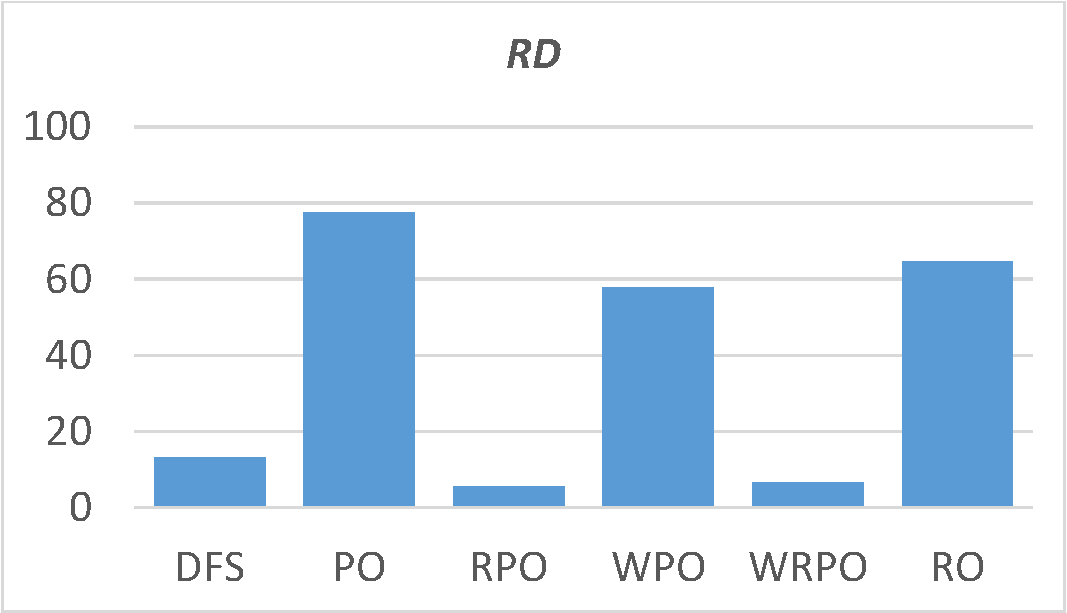
\includegraphics[width=0.32\linewidth]{ecoop-figures/rd-crop.pdf}
%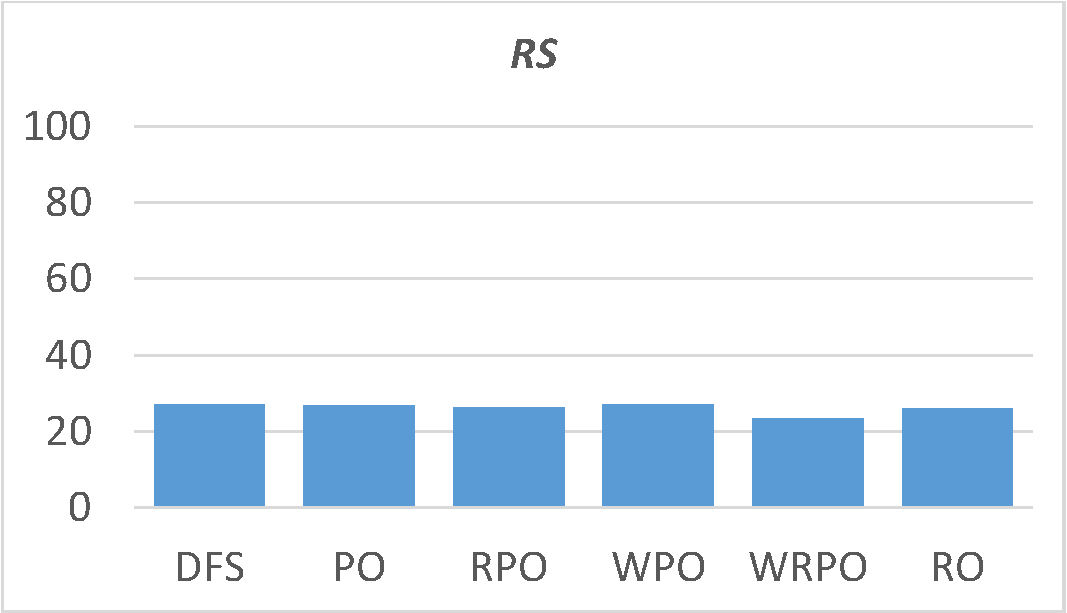
\includegraphics[width=0.32\linewidth]{ecoop-figures/rs-crop.pdf}
%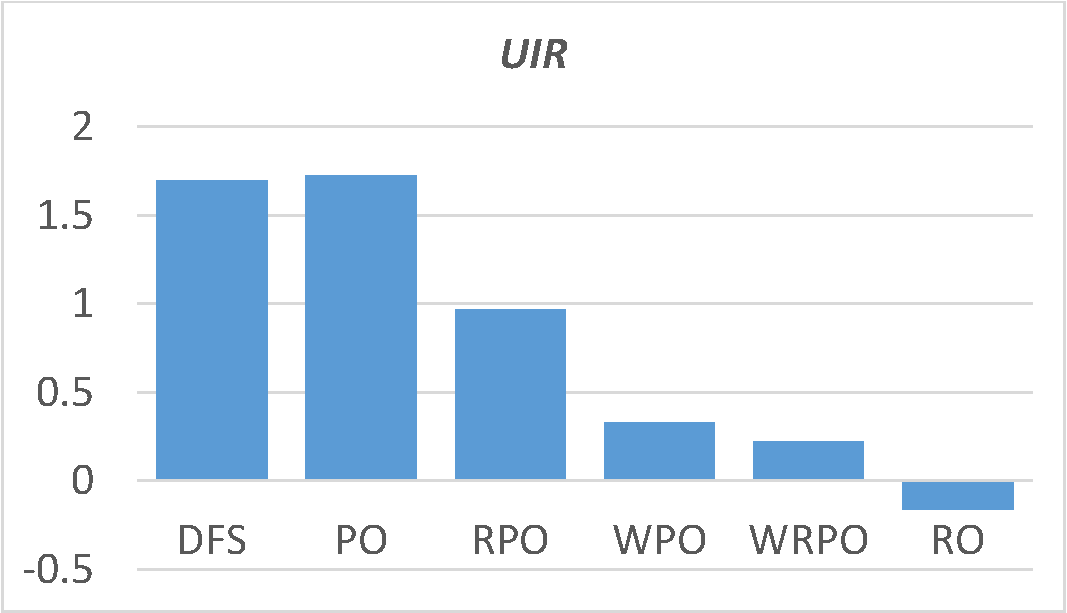
\includegraphics[width=0.32\linewidth]{ecoop-figures/uir-crop.pdf}
%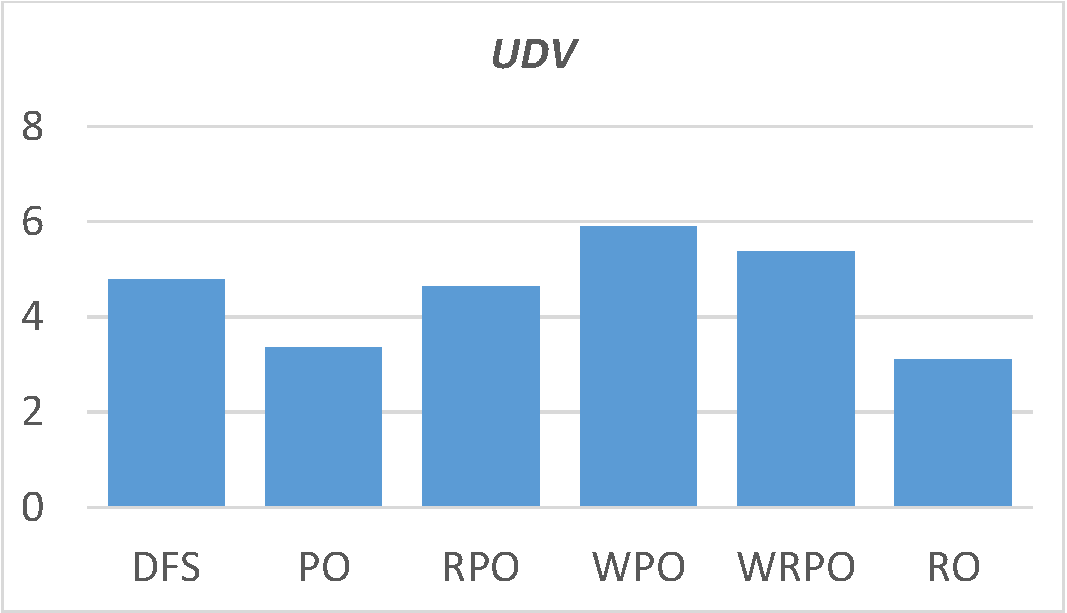
\includegraphics[width=0.32\linewidth]{ecoop-figures/udv-crop.pdf}
%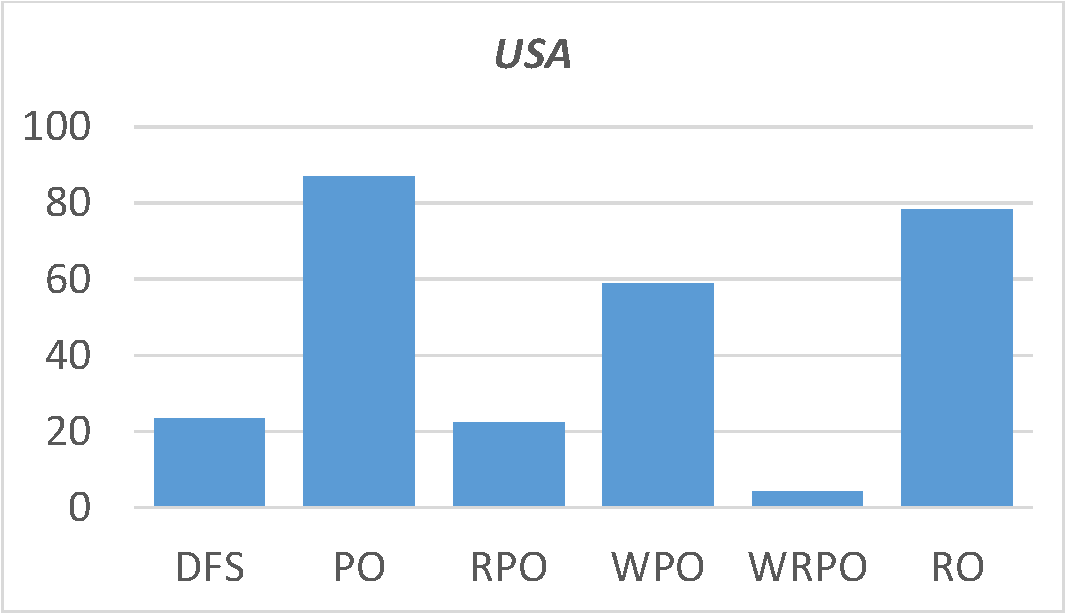
\includegraphics[width=0.32\linewidth]{ecoop-figures/usa-crop.pdf}
%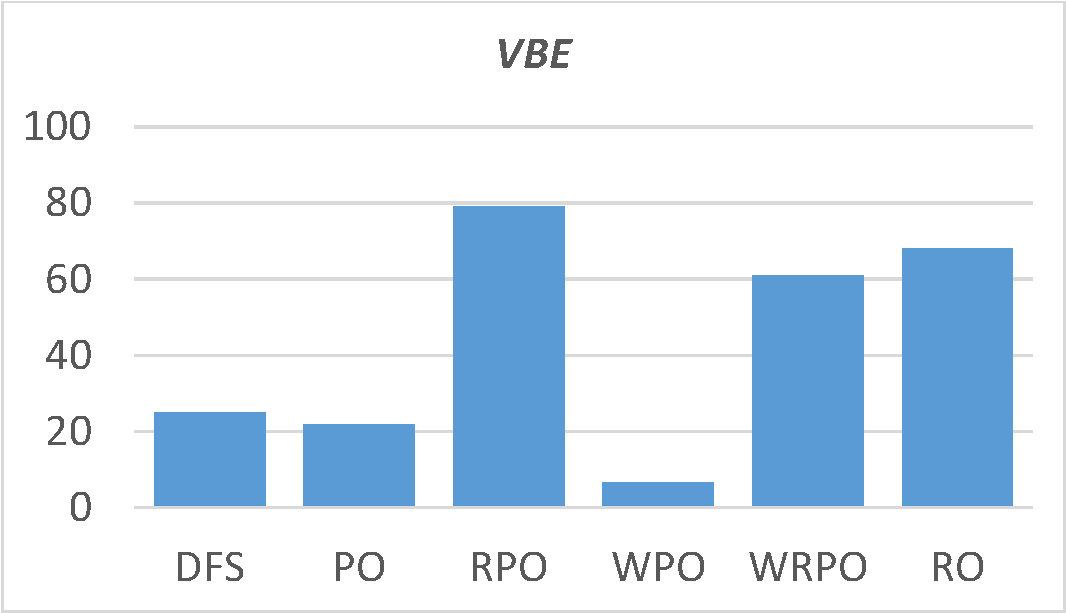
\includegraphics[width=0.32\linewidth]{ecoop-figures/vbe-crop.pdf}
%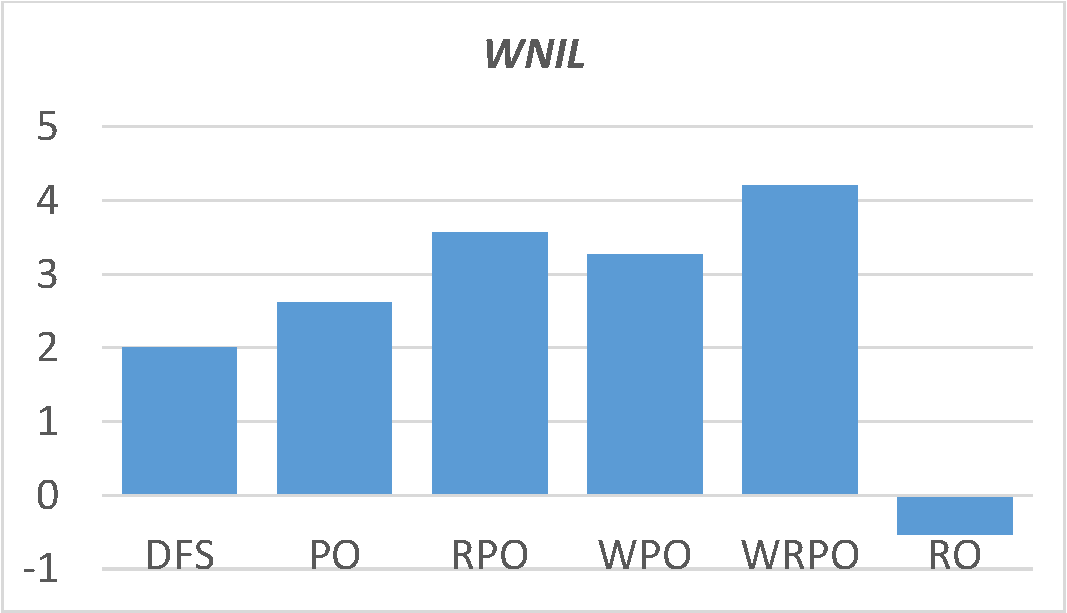
\includegraphics[width=0.32\linewidth]{ecoop-figures/wnil-crop.pdf}\newline
%\textbf{c) \textit{Overall}}\\
%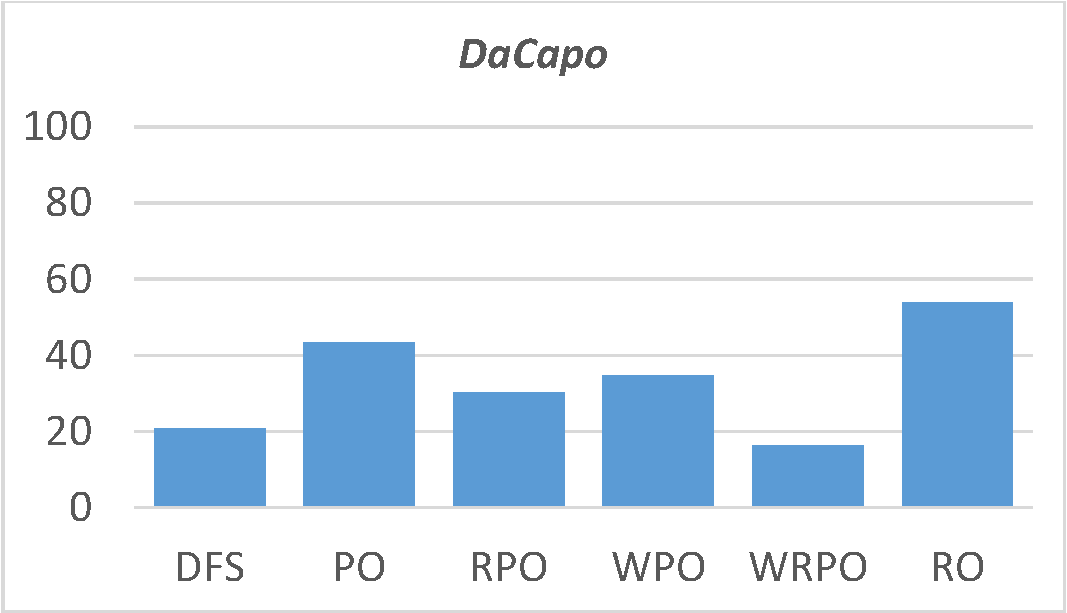
\includegraphics[width=0.32\linewidth]{ecoop-figures/dacapo-overall-crop.pdf}
  %\caption[Percentage reduction in execution time of hybrid approach over other candidate traversals on \textit{DaCapo} (Sequential mode) and \textit{SourceForge} (Cluster mode).]
%{Percentage reduction in execution time of hybrid approach over other candidate traversals on \textit{DaCapo} (Sequential mode) and \textit{SourceForge} (Cluster mode).
%\label{fig:dacapo-singlemachine-time-percentage}}
%\end{figure*}

%\begin{figure*}[ht!]
%\centering
%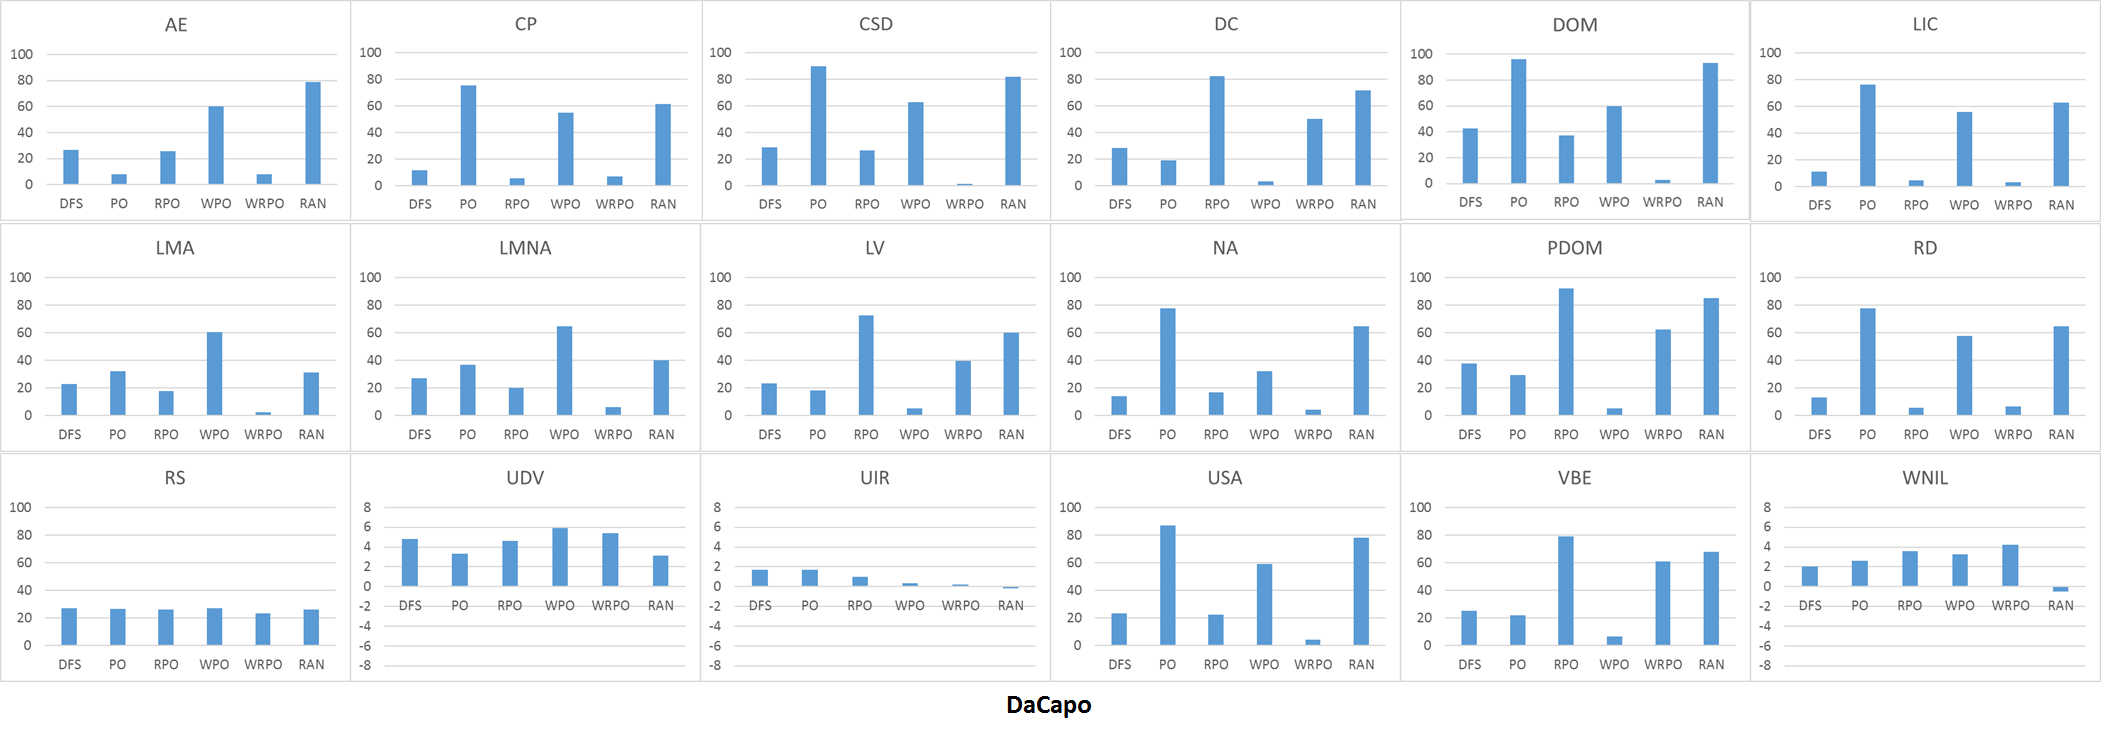
\includegraphics[width=\textwidth]{ecoop-figures/dacapo-seq-reduction.png}
%  \caption[Percentage reduction in execution time of hybrid approach over other candidate traversals on \textit{DaCapo} (Sequential mode), \textit{DaCapo} (Cluster mode), \textit{SourceForge} (Cluster mode).]
%{Percentage reduction in execution time of hybrid approach over other candidate traversals on \textit{DaCapo} (Sequential mode), \textit{DaCapo} (Cluster mode), \textit{SourceForge} (Cluster mode).
%\label{fig:dacapo-singlemachine-time-percentage}}
%\end{figure*}

\begin{figure}%
\centering
\scriptsize
\begin{tabular}{lrrrrrr|rrrrrr}
\toprule
\multicolumn{1}{l}{Analysis} & \multicolumn{1}{c|}{DaCapo}                    & \multicolumn{1}{c}{GitHub} \\
\midrule
\multicolumn{1}{l}{CP} & \cellcolor{lightblue}9\%  & \cellcolor{lightblue}5\%  \\
\multicolumn{1}{l}{CSD} & \cellcolor{lightblue}4\%  & \cellcolor{lightblack}12\% \\
\multicolumn{1}{l}{DC} & \cellcolor{lightblue}7\%  & \cellcolor{lightblue}7\%  \\
\multicolumn{1}{l}{LIC} & \cellcolor{lightblue}7\%  & \cellcolor{lightblack}19\% \\
\multicolumn{1}{l}{USA} & \cellcolor{lightblue}9\%  & \cellcolor{lightblue}9\% \\
\multicolumn{1}{l}{VFR} & \cellcolor{lightblack}15\%  & \cellcolor{lightblue}9\% \\
\multicolumn{1}{l}{MWN} & \cellcolor{lightblack}15\%  & \cellcolor{lightblue}9\% \\
\multicolumn{1}{l}{AE} & \cellcolor{lightblack}14\%  &  \cellcolor{lightblack}11\% \\
\multicolumn{1}{l}{DOM} & \cellcolor{lightblue}6\%  & \cellcolor{lightblue}6\% \\
\multicolumn{1}{l}{LMA} & \cellcolor{lightblue}6\%  & \cellcolor{lightblue}6\% \\
\multicolumn{1}{l}{LMNA} & \cellcolor{lightblue}9\%  & \cellcolor{lightblue}7\% \\
\multicolumn{1}{l}{LV} & \cellcolor{lightblack}11\%  & \cellcolor{lightblack}11\%  \\
\multicolumn{1}{l}{NA} & \cellcolor{lightblack}10\%  & \cellcolor{lightblack}10\%  \\
\multicolumn{1}{l}{PDOM} & \cellcolor{lightblack}10\%  & \cellcolor{lightblack}24\% \\
\multicolumn{1}{l}{RD} & \cellcolor{lightblue}9\%  & \cellcolor{lightblue}5\% \\
\multicolumn{1}{l}{RS} & \cellcolor{lightblack}28\%  & \cellcolor{lightblue}7\% \\
\multicolumn{1}{l}{VBE} & \cellcolor{lightblack}13\%  & \cellcolor{lightblack}10\% \\
\multicolumn{1}{l}{SS} & \cellcolor{lightblack}22\%  & \cellcolor{lightblack}10\%  \\
\multicolumn{1}{l}{UDV} &  \cellcolor{lightblue}3\%   &  \cellcolor{lightblue}0\%  \\
\multicolumn{1}{l}{UIR} &  \cellcolor{lightblue}0\%   &  \cellcolor{lightblue}0\%  \\
\multicolumn{1}{l}{WNIL} &  \cellcolor{lightblue}2\%   &  \cellcolor{lightblue}0\% \\
\bottomrule
\end{tabular}%
\caption{Reduction in running times against hand optimized analysis.}
\label{fig:reduction-oopsla}
\end{figure}


Another way to extract more performance is to hand optimize the analysis.
\fignref{fig:reduction-oopsla} compares Hybrid approach against hand optimized analysis. Hand optimized analysis has single best optimized traversal strategy applied for each analysis. For data-flow analysis, hand optimized analysis uses WPO/WRPO guideline while for non data flow analysis, it uses ANY traversal strategy, as it is the best traversal strategy for non data-flow analysis. WPO/WRPO guideline suggests that if the direction of the traversal is backward, use WPO else use WRPO. This guideline  
simplifies the hybrid approach, where the decision is based on only traversal 
direction while Hybrid approach uses the decision tree in \fignref{fig:decision-diagram}. 
\fignref{fig:reduction-oopsla} shows the 
comparison of hybrid approach against hand optimized analysis. We can see that for 
about half of the data-flow analysis, we gain at least 10\% reduction. For analysis like 
RS, SS, VFR and MWN, the gain is much higher since these analyses are 
selective in terms of the program statements that they analyze. WPO and WRPO 
would not work for these analyses since in case of both WPO and WRPO, there 
exists a fixed cost of creating and maintaining a worklist of size equals to 
the number of CFG nodes. When analyses selectively analyzes a small subset of 
all nodes in the CFGs, this overhead becomes substantial. Our hybrid strategy 
is not only able to select an alternative strategy instead of WPO/WRPO for 
such selective analyses, whenever possible (when the input graphs do not 
contain loops), but also optimize WPO/WRPO (in case of input graphs with loops), 
such that the overheads are minimized.
For non-data flow analysis, there is no gain against hand optimized analysis since ANY is the best traversal strategy for such analysis and both Hybrid approach and hand optimized analysis applied ANY traversal strategy for all the graphs for non-data flow analysis.
\section{Correctness of Analysis Results}
\label{sec:soundness}

To evaluate the correctness of analysis results, we first chose worklist 
as standard strategy to run analyses on DaCapo dataset to create the 
groundtruth of the results. We then ran analyses using our hybrid approach 
and compared the results with the groundtruth. In all analyses on all 
input graphs from the dataset, the results from our hybrid approach always 
exactly matched the corresponding ones in the groundtruth. 
%\todo{That means the 
%hybrid approach does not compromise on the correctness of the result while 
%picking and optimizing the best traversal strategy.} 

\section{Traversal Strategy Selection Precision}
\label{sec:prediction-accuracy}

% Table generated by Excel2LaTeX from sheet 'Sheet1'
\begin{table}
\footnotesize
\centering
\caption{Traversal strategy prediction precision.}
\setlength{\tabcolsep}{2pt}
\begin{tabular}{cr}
\toprule
Analysis & Precision \\
\midrule
DOM, PDOM, WNIL, UDV, UIR & 100.00\% \\
CP, CSD, DC, LIC, USA, VFR, MWN, AE, LMA, LMNA, LV, NA, RD, RS, VBE, SS  & 99.99\% \\
\bottomrule
\end{tabular}%
\label{tab:prediction-precision}%
\end{table}%

\begin{figure}[h]
\centering
\subfloat[CP]{
\fbox{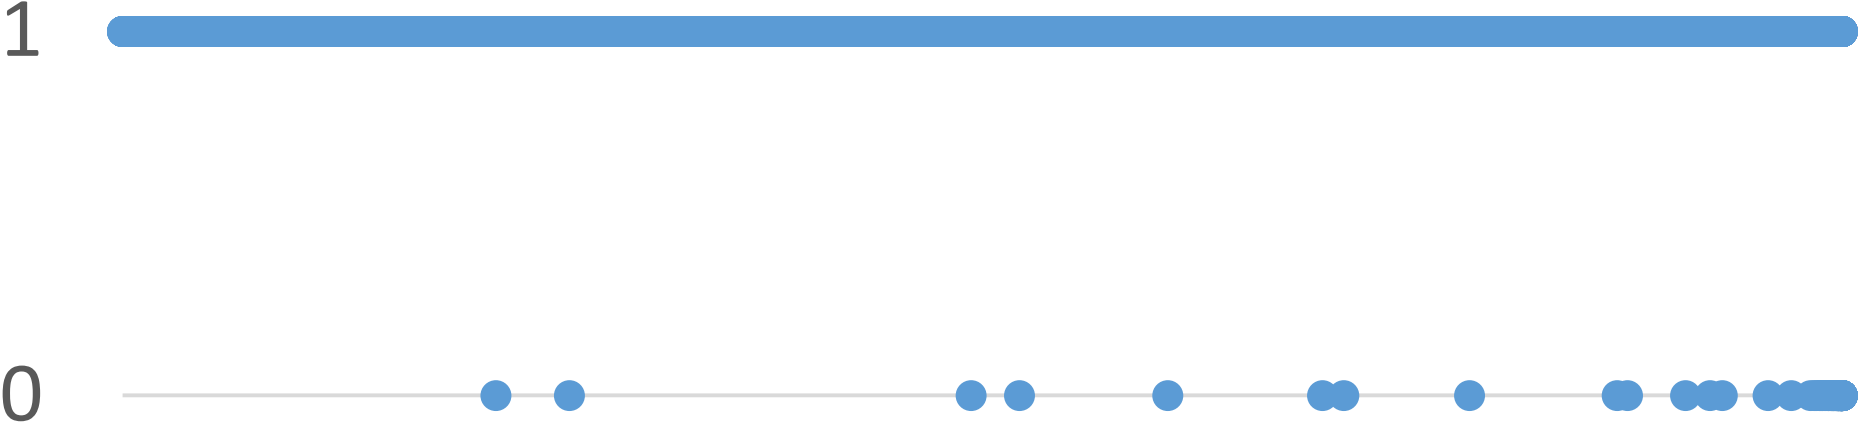
\includegraphics[width=0.22\linewidth]{figures/loop-cp.png}}
\label{fig:loop-cp}
}
\subfloat[CSD]{
\fbox{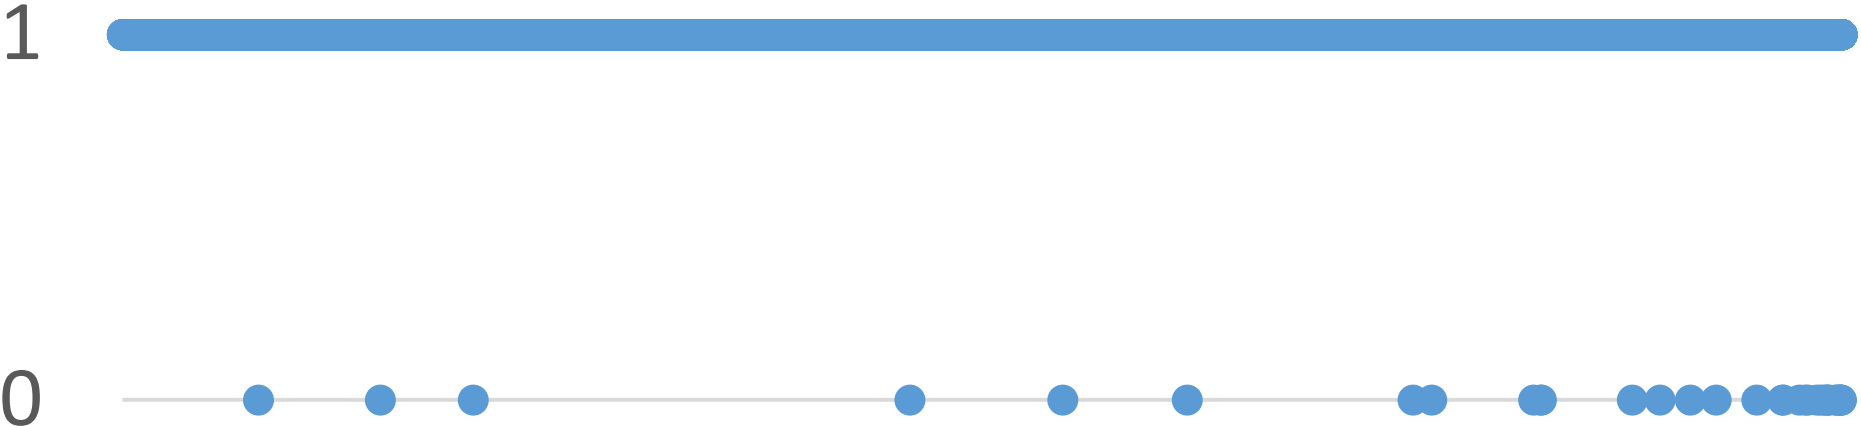
\includegraphics[width=0.22\linewidth]{figures/loop-csd.png}}
\label{fig:loop-csd}
}
\subfloat[DC]{
\fbox{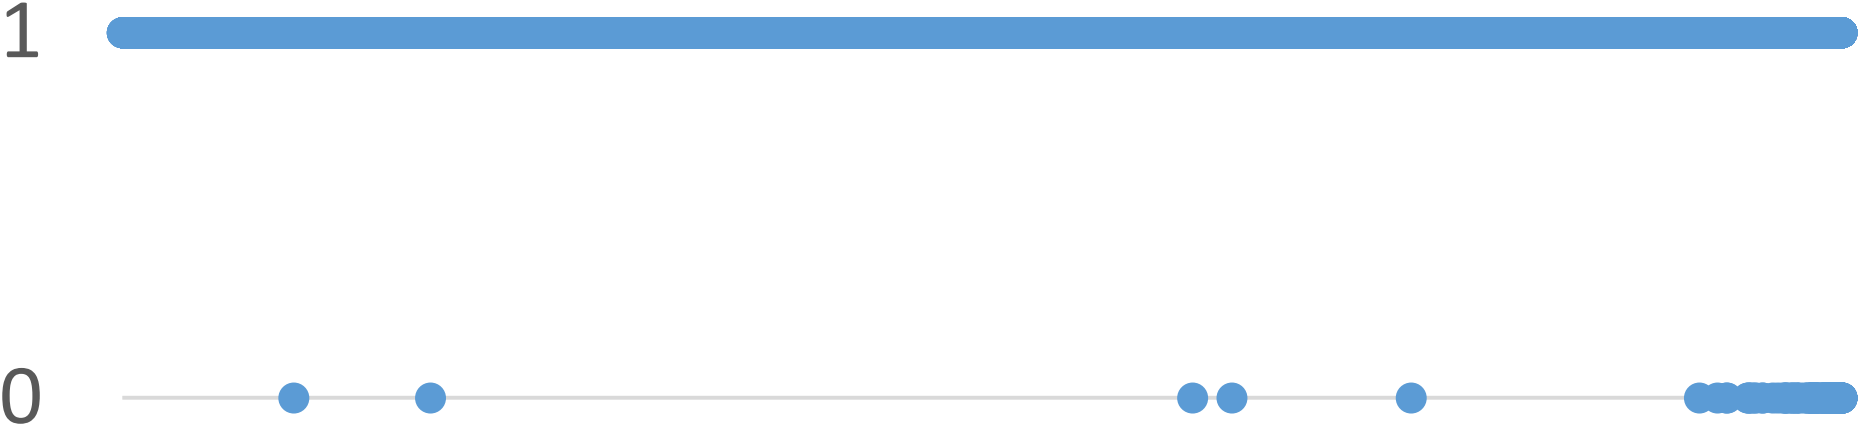
\includegraphics[width=0.22\linewidth]{figures/loop-dc.png}}
\label{fig:loop-dc}
}
\subfloat[LIC]{
\fbox{\includegraphics[width=0.22\linewidth]{figures/loop-lic.png}}
\label{fig:loop-lic}
}\\
\subfloat[USA]{
\fbox{\includegraphics[width=0.22\linewidth]{figures/loop-usa.png}}
\label{fig:loop-use}
}
\subfloat[VFR]{
	\fbox{\includegraphics[width=0.22\linewidth]{figures/loop-vfr.png}}
	\label{fig:loop-vfr}
}
\subfloat[MWN]{
	\fbox{\includegraphics[width=0.22\linewidth]{figures/loop-mwn.png}}
	\label{fig:loop-mwn}
}
\subfloat[AE]{
\fbox{\includegraphics[width=0.22\linewidth]{figures/loop-ae.png}}
\label{fig:loop-ae}
}\\
\subfloat[LMA]{
\fbox{\includegraphics[width=0.22\linewidth]{figures/loop-lma.png}}
\label{fig:loop-lma}
}
\subfloat[LMNA]{
\fbox{\includegraphics[width=0.22\linewidth]{figures/loop-lmna.png}}
\label{fig:loop-lmna}
}
\subfloat[LV]{
\fbox{\includegraphics[width=0.22\linewidth]{figures/loop-lv.png}}
\label{fig:loop-lv}
}
\subfloat[NA]{
\fbox{\includegraphics[width=0.22\linewidth]{figures/loop-na.png}}
\label{fig:loop-na}
}\\
\subfloat[RD]{
\fbox{\includegraphics[width=0.22\linewidth]{figures/loop-rd.png}}
\label{fig:loop-rd}
}
\subfloat[RS]{
\fbox{\includegraphics[width=0.22\linewidth]{figures/loop-rs.png}}
\label{fig:loop-rs}
}
\subfloat[VBE]{
\fbox{\includegraphics[width=0.22\linewidth]{figures/loop-vbe.png}}
\label{fig:loop-vbe}
}
\subfloat[SS]{
	\fbox{\includegraphics[width=0.22\linewidth]{figures/loop-ss.png}}
	\label{fig:loop-ss}
}\\
\caption{Scatter charts for analyses that have loop sensitive traversals. 
%$x$-axis lists the CFGs in the increasing of the node size. 
}
\label{fig:loops}
\end{figure}



In this experiment, we evaluated how well the hybrid approach picks the most 
time-efficient strategy. We ran the 21 analyses on the DaCapo dataset using 
all the candidate traversals and the one selected by the hybrid approach. One 
selection is counted for each pair of a traversal and an input graph where 
the hybrid approach selects a traversal strategy based on the properties of 
the analysis and input graph. A selection is considered correct if its 
running time is at least as good as the running time of the fastest among all 
candidates. The precision is computed as the ratio between the number of 
correct selections over the total number of all selections. 
%
As shown in \tabref{tab:prediction-precision}, the selection precision is 100\% 
for all analyses that are not \textit{loop sensitive}. For analyses that 
involve \textit{loop sensitive} traversals, the prediction precision is 99.99\%. 

We further analyzed the result to see what contributed to these mispredictions. 
Let us break the CFGs in the DaCapo dataset by the graph \graphprop{}: sequential CFGs, 
CFGs with branches and no loops, and CFGs with loops, and discuss the selection precision.

For \textbf{sequential CFGs \& CFGs with branches and no loops}, the selection  
precision is 100\%---the hybrid approach always picks the most time-efficient 
traversal strategy.

For \textbf{CFGs with loops}, the selection precision is 100\% for \emph{loop 
	insensitive} traversals. The mispredictions occur with \emph{loop sensitive} 
traversals on CFGs with loops. Figure \ref{fig:loops} shows scatter charts 
for the traversal selection results for 16 analyses that are \textit{loop 
	sensitive}. In the chart, 1 indicates a correct selection and 0 indicates a 
misprediction. CFGs are organized along the $x$- axis in the increasing order 
of their sizes measured as the numbers of nodes. 
%
The scatter charts show that the mispredictions tend to happen with larger 
CFGs. 
%
The reason is that, for \textit{loop sensitive} traversals, the hybrid 
approach picks worklist as the best strategy. The worklist approach was 
picked because it visits only as many nodes as needed when compared to other 
traversal strategies which visit redundant nodes. However using worklist 
imposes an overhead of creating and maintaining a worklist containing all 
nodes in the CFG. This overhead is negligible for small CFGs. However, when 
running analyses on large CFGs, this overhead could become higher 
than the cost for visiting redundant nodes. Therefore, selecting worklist for 
\emph{loop sensitive} traversals on large CFGs might not always result in the 
best running times. 

\begin{figure}[h]
\centering

\includegraphics[width=0.32\linewidth]{tex-figures/misprediction/cp-crop.pdf}
\label{fig:mis-cp}
\includegraphics[width=0.32\linewidth]{tex-figures/misprediction/csd-crop.pdf}
\label{fig:mis-csd}
\includegraphics[width=0.32\linewidth]{tex-figures/misprediction/DC-crop.pdf}
\label{fig:mis-dc}
\\
\includegraphics[width=0.32\linewidth]{tex-figures/misprediction/LIC-crop.pdf}
\label{fig:mis-lic}
\includegraphics[width=0.32\linewidth]{tex-figures/misprediction/usa-crop.pdf}
\label{fig:mis-use}
	\includegraphics[width=0.32\linewidth]{tex-figures/misprediction/vfr-crop.pdf}
	\label{fig:mis-vfr}
	\\
	\includegraphics[width=0.32\linewidth]{tex-figures/misprediction/mwn-crop.pdf}
	\label{fig:mis-mwn}
\includegraphics[width=0.32\linewidth]{tex-figures/misprediction/AE-crop.pdf}
\label{fig:mis-ae}
\includegraphics[width=0.32\linewidth]{tex-figures/misprediction/LMA-crop.pdf}
\label{fig:mis-lma}
\\
\includegraphics[width=0.32\linewidth]{tex-figures/misprediction/LMNA-crop.pdf}
\label{fig:mis-lmna}
\includegraphics[width=0.32\linewidth]{tex-figures/misprediction/LV-crop.pdf}
\label{fig:mis-lv}
\includegraphics[width=0.32\linewidth]{tex-figures/misprediction/NA-crop.pdf}
\label{fig:mis-na}
\\
\includegraphics[width=0.32\linewidth]{tex-figures/misprediction/rd-crop.pdf}
\label{fig:mis-rd}
\includegraphics[width=0.32\linewidth]{tex-figures/misprediction/rs-crop.pdf}
\label{fig:mis-rs}
\includegraphics[width=0.32\linewidth]{tex-figures/misprediction/VBE-crop.pdf}
\label{fig:mis-vbe}
\\
	\includegraphics[width=0.32\linewidth]{tex-figures/misprediction/SS-crop.pdf}
	\label{fig:mis-ss}
\caption{Hybrid approach's performance against best approaches for mis-predicted graphs.}
\label{fig:mis-graph}
\end{figure}


%\begin{figure}
%	\centering
%	\includegraphics[width=0.50\linewidth]{tex-figures/loop-ae-ns.pdf}
%	\caption{Hybrid approach's performance against best approaches for mis-predicted graphs.}%
%	\label{fig:loop-ae-ns}%
%\end{figure}

\fignref{fig:mis-graph} shows the Hybrid approach's performance against best 
approaches for mis-predicted graphs for 16 analyses that has \emph{loop sensitive} traversals. We can see that for 
majority of the mis-predicted graphs, Hybrid approach's performance is 
comparable to the best approaches. 
%As graph's size increases, Hybrid's performance for mis-predicted graphs worsens and is no more comparable to the best approach. 

\section{Analysis on the Decision Tree Distribution}
\label{sec:analysis-decision-tree}

\begin{figure*}
	\centering
	\scriptsize
\begin{tabular}{lrrrrrrrrrrr}
\toprule
      & P1    & P2    & P3    & P4    & P5    & P6    & P7    & P8    & P9    & P10   & P11 \\
\midrule
CP    & \cellcolor{lightgreen}35\%   & \cellcolor{lightred}0\%   & \cellcolor{lightgreen}10\%   & \cellcolor{lightred}0\%   & \cellcolor{lightred}0\%   & \cellcolor{lightred}0\%   & \cellcolor{lightred}0\%   & \cellcolor{lightred}0\%   & \cellcolor{lightblack}5\%   & \cellcolor{lightred}0\%   & \cellcolor{lightgreen}50\% \\
CSD   & \cellcolor{lightgreen}35\%   & \cellcolor{lightred}0\%   & \cellcolor{lightgreen}10\%   & \cellcolor{lightred}0\%   & \cellcolor{lightred}0\%   & \cellcolor{lightred}0\%   & \cellcolor{lightred}0\%   & \cellcolor{lightred}0\%   & \cellcolor{lightblack}5\%   & \cellcolor{lightred}0\%   & \cellcolor{lightgreen}50\% \\
DC    & \cellcolor{lightred}0\%   & \cellcolor{lightgreen}35\%   & \cellcolor{lightred}0\%   & \cellcolor{lightgreen}10\%   & \cellcolor{lightred}0\%   & \cellcolor{lightred}0\%   & \cellcolor{lightred}0\%   & \cellcolor{lightred}0\%   & \cellcolor{lightred}0\%   & \cellcolor{lightblack}5\%   & \cellcolor{lightgreen}50\% \\
LIC   & \cellcolor{lightgreen}35\%   & \cellcolor{lightred}0\%   & \cellcolor{lightgreen}10\%   & \cellcolor{lightred}0\%   & \cellcolor{lightred}0\%   & \cellcolor{lightred}0\%   & \cellcolor{lightred}0\%   & \cellcolor{lightred}0\%   & \cellcolor{lightblack}5\%   & \cellcolor{lightred}0\%   & \cellcolor{lightgreen}50\% \\
USA   & \cellcolor{lightgreen}35\%   & \cellcolor{lightred}0\%   & \cellcolor{lightgreen}10\%   & \cellcolor{lightred}0\%   & \cellcolor{lightred}0\%   & \cellcolor{lightred}0\%   & \cellcolor{lightred}0\%   & \cellcolor{lightred}0\%   & \cellcolor{lightblack}5\%   & \cellcolor{lightred}0\%   & \cellcolor{lightgreen}50\% \\
VFR   & \cellcolor{lightgreen}35\%   & \cellcolor{lightred}0\%   & \cellcolor{lightgreen}10\%   & \cellcolor{lightred}0\%   & \cellcolor{lightred}0\%   & \cellcolor{lightred}0\%   & \cellcolor{lightred}0\%   & \cellcolor{lightred}0\%   & \cellcolor{lightblack}5\%   & \cellcolor{lightred}0\%   & \cellcolor{lightgreen}50\% \\
MWN   & \cellcolor{lightgreen}35\%   & \cellcolor{lightred}0\%   & \cellcolor{lightgreen}10\%   & \cellcolor{lightred}0\%   & \cellcolor{lightred}0\%   & \cellcolor{lightred}0\%   & \cellcolor{lightred}0\%   & \cellcolor{lightred}0\%   & \cellcolor{lightblack}5\%   & \cellcolor{lightred}0\%   & \cellcolor{lightgreen}50\% \\
AE    & \cellcolor{lightgreen}69\%   & \cellcolor{lightred}0\%   & \cellcolor{lightgreen}21\%   & \cellcolor{lightred}0\%   & \cellcolor{lightred}0\%   & \cellcolor{lightred}0\%   & \cellcolor{lightred}0\%   & \cellcolor{lightred}0\%   & \cellcolor{lightgreen}10\%   & \cellcolor{lightred}0\%   & \cellcolor{lightred}0\% \\
DOM   & \cellcolor{lightgreen}69\%   & \cellcolor{lightred}0\%   & \cellcolor{lightgreen}21\%   & \cellcolor{lightred}0\%   & \cellcolor{lightblack}7\%   & \cellcolor{lightred}0\%   & \cellcolor{lightblack}3\%   & \cellcolor{lightred}0\%   & \cellcolor{lightred}0\%   & \cellcolor{lightred}0\%   & \cellcolor{lightred}0\% \\
LMA   & \cellcolor{lightgreen}69\%   & \cellcolor{lightred}0\%   & \cellcolor{lightgreen}21\%   & \cellcolor{lightred}0\%   & \cellcolor{lightred}0\%   & \cellcolor{lightred}0\%   & \cellcolor{lightred}0\%   & \cellcolor{lightred}0\%   & \cellcolor{lightgreen}10\%   & \cellcolor{lightred}0\%   & \cellcolor{lightred}0\% \\
LMNA  & \cellcolor{lightgreen}69\%   & \cellcolor{lightred}0\%   & \cellcolor{lightgreen}21\%   & \cellcolor{lightred}0\%   & \cellcolor{lightred}0\%   & \cellcolor{lightred}0\%   & \cellcolor{lightred}0\%   & \cellcolor{lightred}0\%   & \cellcolor{lightgreen}10\%   & \cellcolor{lightred}0\%   & \cellcolor{lightred}0\% \\
LV    & \cellcolor{lightred}0\%   & \cellcolor{lightgreen}69\%   & \cellcolor{lightred}0\%   & \cellcolor{lightgreen}21\%   & \cellcolor{lightred}0\%   & \cellcolor{lightred}0\%   & \cellcolor{lightred}0\%   & \cellcolor{lightred}0\%   & \cellcolor{lightred}0\%   & \cellcolor{lightgreen}10\%   & \cellcolor{lightred}0\% \\
NA    & \cellcolor{lightgreen}69\%   & \cellcolor{lightred}0\%   & \cellcolor{lightgreen}21\%   & \cellcolor{lightred}0\%   & \cellcolor{lightred}0\%   & \cellcolor{lightred}0\%   & \cellcolor{lightred}0\%   & \cellcolor{lightred}0\%   & \cellcolor{lightgreen}10\%   & \cellcolor{lightred}0\%   & \cellcolor{lightred}0\% \\
PDOM  & \cellcolor{lightred}0\%   & \cellcolor{lightgreen}69\%   & \cellcolor{lightred}0\%   & \cellcolor{lightgreen}21\%   & \cellcolor{lightred}0\%   & \cellcolor{lightblack}7\%   & \cellcolor{lightred}0\%   & \cellcolor{lightblack}3\%   & \cellcolor{lightred}0\%   & \cellcolor{lightred}0\%   & \cellcolor{lightred}0\% \\
RD    & \cellcolor{lightgreen}69\%   & \cellcolor{lightred}0\%   & \cellcolor{lightgreen}21\%   & \cellcolor{lightred}0\%   & \cellcolor{lightred}0\%   & \cellcolor{lightred}0\%   & \cellcolor{lightred}0\%   & \cellcolor{lightred}0\%   & \cellcolor{lightgreen}10\%   & \cellcolor{lightred}0\%   & \cellcolor{lightred}0\% \\
RS    & \cellcolor{lightgreen}69\%   & \cellcolor{lightred}0\%   & \cellcolor{lightgreen}21\%   & \cellcolor{lightred}0\%   & \cellcolor{lightred}0\%   & \cellcolor{lightred}0\%   & \cellcolor{lightred}0\%   & \cellcolor{lightred}0\%   & \cellcolor{lightgreen}10\%   & \cellcolor{lightred}0\%   & \cellcolor{lightred}0\% \\
VBE   & \cellcolor{lightred}0\%   & \cellcolor{lightgreen}69\%   & \cellcolor{lightred}0\%   & \cellcolor{lightgreen}21\%   & \cellcolor{lightred}0\%   & \cellcolor{lightred}0\%   & \cellcolor{lightred}0\%   & \cellcolor{lightred}0\%   & \cellcolor{lightred}0\%   & \cellcolor{lightgreen}10\%   & \cellcolor{lightred}0\% \\
SS    & \cellcolor{lightgreen}69\%   & \cellcolor{lightred}0\%   & \cellcolor{lightgreen}21\%   & \cellcolor{lightred}0\%   & \cellcolor{lightred}0\%   & \cellcolor{lightred}0\%   & \cellcolor{lightred}0\%   & \cellcolor{lightred}0\%   & \cellcolor{lightgreen}10\%   & \cellcolor{lightred}0\%   & \cellcolor{lightred}0\% \\
UDV   & \cellcolor{lightred}0\%   & \cellcolor{lightred}0\%   & \cellcolor{lightred}0\%   & \cellcolor{lightred}0\%   & \cellcolor{lightred}0\%   & \cellcolor{lightred}0\%   & \cellcolor{lightred}0\%   & \cellcolor{lightred}0\%   & \cellcolor{lightred}0\%   & \cellcolor{lightred}0\%   & \cellcolor{lightgreen}100\% \\
UIR   & \cellcolor{lightred}0\%   & \cellcolor{lightred}0\%   & \cellcolor{lightred}0\%   & \cellcolor{lightred}0\%   & \cellcolor{lightred}0\%   & \cellcolor{lightred}0\%   & \cellcolor{lightred}0\%   & \cellcolor{lightred}0\%   & \cellcolor{lightred}0\%   & \cellcolor{lightred}0\%   & \cellcolor{lightgreen}100\% \\
WNIL  & \cellcolor{lightred}0\%   & \cellcolor{lightred}0\%   & \cellcolor{lightred}0\%   & \cellcolor{lightred}0\%   & \cellcolor{lightred}0\%   & \cellcolor{lightred}0\%   & \cellcolor{lightred}0\%   & \cellcolor{lightred}0\%   & \cellcolor{lightred}0\%   & \cellcolor{lightred}0\%   & \cellcolor{lightgreen}100\% \\
\midrule
Overall & \cellcolor{lightgreen}34.54\%   & \cellcolor{lightgreen}9.87\%   & \cellcolor{lightblack}10.32\%   & \cellcolor{lightblack}2.95\%   & \cellcolor{lightblue}0.26\%   & \cellcolor{lightblue}0.26\%   & \cellcolor{lightblue}0.11\%   & \cellcolor{lightblue}0.11\%   & \cellcolor{lightblack}4.78\%   & \cellcolor{lightblack}1.10\%   & \cellcolor{lightgreen}35.71\% \\
\bottomrule
\end{tabular}%
	\caption{Distribution of decisions over the paths of the decision tree.}
	\label{fig:decision-distribution}
	\label{fig:paths-sf}
\end{figure*}

%\begin{table}%
%\centering
%\scriptsize
%\caption{Reduction in running times. Background colors indicate the ranges of 
%values: \colorbox{lightred}{0\%}, \colorbox{lightblue}{(0\%, 1\%)}, 
%\colorbox{lightblack}{[1\%, 10\%)} and \colorbox{lightgreen}{[10\%, 100\%]}.}
%\begin{tabular}{lrrrrrrrrrrr}
%\toprule
      %& P1    & P2    & P3    & P4    & P5    & P6    & P7    & P8    & P9    & P10   & P11 \\
%\midrule
%CP    & 32\%  & 0\%   & 13\%  & 0\%   & 0\%   & 0\%   & 0\%   & 0\%   & 5\%   & 0\%   & 50\% \\
%CSD   & 32\%  & 0\%   & 13\%  & 0\%   & 0\%   & 0\%   & 0\%   & 0\%   & 5\%   & 0\%   & 50\% \\
%DC    & 0\%   & 32\%  & 0\%   & 13\%  & 0\%   & 0\%   & 0\%   & 0\%   & 0\%   & 5\%   & 50\% \\
%USA   & 22\%  & 0\%   & 8\%   & 0\%   & 0\%   & 0\%   & 0\%   & 0\%   & 3\%   & 0\%   & 67\% \\
%AE    & 65\%  & 0\%   & 25\%  & 0\%   & 0\%   & 0\%   & 0\%   & 0\%   & 10\%  & 0\%   & 0\% \\
%Dom   & 65\%  & 0\%   & 25\%  & 0\%   & 7\%   & 0\%   & 2\%   & 0\%   & 0\%   & 0\%   & 0\% \\
%LIC   & 22\%  & 0\%   & 8\%   & 0\%   & 0\%   & 0\%   & 0\%   & 0\%   & 3\%   & 0\%   & 67\% \\
%LMA   & 65\%  & 0\%   & 25\%  & 0\%   & 0\%   & 0\%   & 0\%   & 0\%   & 10\%  & 0\%   & 0\% \\
%LMNA  & 65\%  & 0\%   & 25\%  & 0\%   & 0\%   & 0\%   & 0\%   & 0\%   & 10\%  & 0\%   & 0\% \\
%LV    & 0\%   & 2\%   & 0\%   & 97\%  & 0\%   & 0\%   & 0\%   & 0\%   & 0\%   & 0\%   & 0\% \\
%NA    & 65\%  & 0\%   & 25\%  & 0\%   & 0\%   & 0\%   & 0\%   & 0\%   & 10\%  & 0\%   & 0\% \\
%PDOM  & 0\%   & 65\%  & 0\%   & 25\%  & 0\%   & 7\%   & 0\%   & 2\%   & 0\%   & 0\%   & 0\% \\
%RD    & 65\%  & 0\%   & 25\%  & 0\%   & 0\%   & 0\%   & 0\%   & 0\%   & 10\%  & 0\%   & 0\% \\
%RS    & 65\%  & 0\%   & 25\%  & 0\%   & 0\%   & 0\%   & 0\%   & 0\%   & 10\%  & 0\%   & 0\% \\
%VBE   & 0\%   & 65\%  & 0\%   & 25\%  & 0\%   & 0\%   & 0\%   & 0\%   & 0\%   & 10\%  & 0\% \\
%UDV   & 0\%   & 0\%   & 0\%   & 0\%   & 0\%   & 0\%   & 0\%   & 0\%   & 0\%   & 0\%   & 100\% \\
%UIR   & 0\%   & 0\%   & 0\%   & 0\%   & 0\%   & 0\%   & 0\%   & 0\%   & 0\%   & 0\%   & 100\% \\
%WNIL  & 0\%   & 0\%   & 0\%   & 0\%   & 0\%   & 0\%   & 0\%   & 0\%   & 0\%   & 0\%   & 100\% \\
%\midrule
%Overall & 13.99\% & 5.09\% & 5.47\% & 53.01\% & 0.14\% & 0.14\% & 0.05\% & 0.05\% & 1.90\% & 0.57\% & 19.59\% \\
%\bottomrule
%\end{tabular}%
%\label{tab:decision-distribution}
%\end{table}

%\begin{figure}[!t]
	%\centering
	%\subfloat[DaCapo] {
		%\includegraphics[width=0.8\linewidth]{ecoop-figures/distribution-decision-dacapo.png}
		%\label{fig:paths-dacapo}
	%}\\
	%\subfloat[SourceForge] {
	%\includegraphics[width=0.8\linewidth]{ecoop-figures/distribution-decision-sf.png}
		%\label{fig:paths-sf}
	%}\\
	%\subfloat[All analyses] {
	%\includegraphics[width=0.8\linewidth]{ecoop-figures/distribution-decision-overall.png}
		%\label{fig:paths-all}
	%}
	%\caption{Distribution of decisions over the paths of the decision tree.}
	%\label{fig:decision-distribution}
%\end{figure}


\begin{figure*}[h]
	\centering
	\scriptsize
	%\setlength{\tabcolsep}{5pt}
\begin{tabular}{lrrrrrrrrrrr}
\toprule
      & P1    & P2    & P3    & P4    & P5    & P6    & P7    & P8    & P9    & P10   & P11 \\
\midrule
CP    & \cellcolor{lightgreen}32\%  & \cellcolor{lightred}0\%   & \cellcolor{lightgreen}13\%  & \cellcolor{lightred}0\%   & \cellcolor{lightred}0\%   & \cellcolor{lightred}\cellcolor{lightred}0\%   & \cellcolor{lightred}0\%   & \cellcolor{lightred}0\%   & \cellcolor{lightblack}5\%   & \cellcolor{lightred}0\%   & \cellcolor{lightgreen}50\% \\
CSD   & \cellcolor{lightgreen}32\%  & \cellcolor{lightred}0\%   & \cellcolor{lightgreen}13\%  & \cellcolor{lightred}0\%   & \cellcolor{lightred}0\%   & \cellcolor{lightred}0\%   & \cellcolor{lightred}0\%   & \cellcolor{lightred}0\%   & \cellcolor{lightblack}5\%   & \cellcolor{lightred}0\%   & \cellcolor{lightgreen}50\% \\
DC    & \cellcolor{lightred}0\%   & \cellcolor{lightgreen}32\%  & \cellcolor{lightred}0\%   & \cellcolor{lightgreen}13\%  & \cellcolor{lightred}0\%   & \cellcolor{lightred}0\%   & \cellcolor{lightred}0\%   & \cellcolor{lightred}0\%   & \cellcolor{lightred}0\%   & \cellcolor{lightblack}5\%   & \cellcolor{lightgreen}50\% \\
LIC   & \cellcolor{lightgreen}32\%  & \cellcolor{lightred}0\%   & \cellcolor{lightgreen}13\%  & \cellcolor{lightred}0\%   & \cellcolor{lightred}0\%   & \cellcolor{lightred}0\%   & \cellcolor{lightred}0\%   & \cellcolor{lightred}0\%   & \cellcolor{lightblack}5\%   & \cellcolor{lightred}0\%   & \cellcolor{lightgreen}50\% \\
USA   & \cellcolor{lightgreen}32\%  & \cellcolor{lightred}0\%   & \cellcolor{lightgreen}13\%  & \cellcolor{lightred}0\%   & \cellcolor{lightred}0\%   & \cellcolor{lightred}0\%   & \cellcolor{lightred}0\%   & \cellcolor{lightred}0\%   & \cellcolor{lightblack}5\%   & \cellcolor{lightred}0\%   & \cellcolor{lightgreen}50\% \\
VFR   & \cellcolor{lightgreen}32\%  & \cellcolor{lightred}0\%   & \cellcolor{lightgreen}13\%  & \cellcolor{lightred}0\%   & \cellcolor{lightred}0\%   & \cellcolor{lightred}0\%   & \cellcolor{lightred}0\%   & \cellcolor{lightred}0\%   & \cellcolor{lightblack}5\%   & \cellcolor{lightred}0\%   & \cellcolor{lightgreen}50\% \\
MWN   & \cellcolor{lightgreen}32\%  & \cellcolor{lightred}0\%   & \cellcolor{lightgreen}13\%  & \cellcolor{lightred}0\%   & \cellcolor{lightred}0\%   & \cellcolor{lightred}0\%   & \cellcolor{lightred}0\%   & \cellcolor{lightred}0\%   & \cellcolor{lightblack}5\%   & \cellcolor{lightred}0\%   & \cellcolor{lightgreen}50\% \\
AE    & \cellcolor{lightgreen}65\%  & \cellcolor{lightred}0\%   & \cellcolor{lightgreen}25\%  & \cellcolor{lightred}0\%   & \cellcolor{lightred}0\%   & \cellcolor{lightred}0\%   & \cellcolor{lightred}0\%   & \cellcolor{lightred}0\%   & \cellcolor{lightgreen}10\%  & \cellcolor{lightred}0\%   & \cellcolor{lightred}0\% \\
DOM   & \cellcolor{lightgreen}65\%  & \cellcolor{lightred}0\%   & \cellcolor{lightgreen}25\%  & \cellcolor{lightred}0\%   & \cellcolor{lightblack}7\%   & \cellcolor{lightred}0\%   & \cellcolor{lightblack}2\%   & \cellcolor{lightred}0\%   & \cellcolor{lightred}0\%   & \cellcolor{lightred}0\%   & \cellcolor{lightred}0\% \\
LMA   & \cellcolor{lightgreen}65\%  & \cellcolor{lightred}0\%   & \cellcolor{lightgreen}25\%  & \cellcolor{lightred}0\%   & \cellcolor{lightred}0\%   & \cellcolor{lightred}0\%   & \cellcolor{lightred}0\%   & \cellcolor{lightred}0\%   & \cellcolor{lightgreen}10\%  & \cellcolor{lightred}0\%   & \cellcolor{lightred}0\% \\
LMNA  & \cellcolor{lightgreen}65\%  & \cellcolor{lightred}0\%   & \cellcolor{lightgreen}25\%  & \cellcolor{lightred}0\%   & \cellcolor{lightred}0\%   & \cellcolor{lightred}0\%   & \cellcolor{lightred}0\%   & \cellcolor{lightred}0\%   & \cellcolor{lightgreen}10\%  & \cellcolor{lightred}0\%   & \cellcolor{lightred}0\% \\
LV   & \cellcolor{lightred}0\%   & \cellcolor{lightgreen}65\%  & \cellcolor{lightred}0\%   & \cellcolor{lightgreen}25\%  & \cellcolor{lightred}0\%   & \cellcolor{lightred}0\%   & \cellcolor{lightred}0\%   & \cellcolor{lightred}0\%   & \cellcolor{lightred}0\%   & \cellcolor{lightgreen}10\%  & \cellcolor{lightred}0\% \\
NA    & \cellcolor{lightgreen}65\%  & \cellcolor{lightred}0\%   & \cellcolor{lightgreen}25\%  & \cellcolor{lightred}0\%   & \cellcolor{lightred}0\%   & \cellcolor{lightred}0\%   & \cellcolor{lightred}0\%   & \cellcolor{lightred}0\%   & \cellcolor{lightgreen}10\%  & \cellcolor{lightred}0\%   & \cellcolor{lightred}0\% \\
PDOM  & \cellcolor{lightred}0\%   & \cellcolor{lightgreen}65\%  & \cellcolor{lightred}0\%   & \cellcolor{lightgreen}25\%  & \cellcolor{lightred}0\%   & \cellcolor{lightblack}7\%   & \cellcolor{lightred}0\%   & \cellcolor{lightblack}2\%   & \cellcolor{lightred}0\%   & \cellcolor{lightred}0\%   & \cellcolor{lightred}0\% \\
RD    & \cellcolor{lightgreen}65\%  & \cellcolor{lightred}0\%   & \cellcolor{lightgreen}25\%  & \cellcolor{lightred}0\%   & \cellcolor{lightred}0\%   & \cellcolor{lightred}0\%   & \cellcolor{lightred}0\%   & \cellcolor{lightred}0\%   & \cellcolor{lightgreen}10\%  & \cellcolor{lightred}0\%   & \cellcolor{lightred}0\% \\
RS    & \cellcolor{lightgreen}65\%  & \cellcolor{lightred}0\%   & \cellcolor{lightgreen}25\%  & \cellcolor{lightred}0\%   & \cellcolor{lightred}0\%   & \cellcolor{lightred}0\%   & \cellcolor{lightred}0\%   & \cellcolor{lightred}0\%   & \cellcolor{lightgreen}10\%  & \cellcolor{lightred}0\%   & \cellcolor{lightred}0\% \\
VBE   & \cellcolor{lightred}0\%   & \cellcolor{lightgreen}65\%  & \cellcolor{lightred}0\%   & \cellcolor{lightgreen}25\%  & \cellcolor{lightred}0\%   & \cellcolor{lightred}0\%   & \cellcolor{lightred}0\%   & \cellcolor{lightred}0\%   & \cellcolor{lightred}0\%   & \cellcolor{lightgreen}10\%  & \cellcolor{lightred}0\% \\
SS    & \cellcolor{lightgreen}65\%  & \cellcolor{lightred}0\%   & \cellcolor{lightgreen}25\%  & \cellcolor{lightred}0\%   & \cellcolor{lightred}0\%   & \cellcolor{lightred}0\%   & \cellcolor{lightred}0\%   & \cellcolor{lightred}0\%   & \cellcolor{lightgreen}10\%  & \cellcolor{lightred}0\%   & \cellcolor{lightred}0\% \\
UDV   & \cellcolor{lightred}0\%   & \cellcolor{lightred}0\%   & \cellcolor{lightred}0\%   & \cellcolor{lightred}0\%   & \cellcolor{lightred}0\%   & \cellcolor{lightred}0\%   & \cellcolor{lightred}0\%   & \cellcolor{lightred}0\%   & \cellcolor{lightred}0\%   & \cellcolor{lightred}0\%   & \cellcolor{lightgreen}100\% \\
UIR   & \cellcolor{lightred}0\%   & \cellcolor{lightred}0\%   & \cellcolor{lightred}0\%   & \cellcolor{lightred}0\%   & \cellcolor{lightred}0\%   & \cellcolor{lightred}0\%   & \cellcolor{lightred}0\%   & \cellcolor{lightred}0\%   & \cellcolor{lightred}0\%   & \cellcolor{lightred}0\%   & \cellcolor{lightgreen}100\% \\
WNIL  & \cellcolor{lightred}0\%   & \cellcolor{lightred}0\%   & \cellcolor{lightred}0\%   & \cellcolor{lightred}0\%   & \cellcolor{lightred}0\%   & \cellcolor{lightred}0\%   & \cellcolor{lightred}0\%   & \cellcolor{lightred}0\%   & \cellcolor{lightred}0\%   & \cellcolor{lightred}0\%   & \cellcolor{lightgreen}100\% \\
\midrule
Overall & \cellcolor{lightgreen}32.46\% & \cellcolor{lightgreen}9.27\% & \cellcolor{lightgreen}12.69\% & \cellcolor{lightblack}3.62\% & \cellcolor{lightblue}0.26\% & \cellcolor{lightblue}0.26\% & \cellcolor{lightblue}0.10\% & \cellcolor{lightblue}0.10\% & \cellcolor{lightblack}4.50\% & \cellcolor{lightblack}1.04\% & \cellcolor{lightgreen}35.70\% \\
\bottomrule
\end{tabular}%
	\caption{Distribution of decisions over the paths of the decision tree for the DaCapo Dataset.}
	\label{fig:paths-dacapo}
\end{figure*}

%\begin{table}%
%\centering
%\scriptsize
%\caption{Reduction in running times. Background colors indicate the ranges of 
%values: \colorbox{lightred}{0\%}, \colorbox{lightblue}{(0\%, 1\%)}, 
%\colorbox{lightblack}{[1\%, 10\%)} and \colorbox{lightgreen}{[10\%, 100\%]}.}
%\begin{tabular}{lrrrrrrrrrrr}
%\toprule
      %& P1    & P2    & P3    & P4    & P5    & P6    & P7    & P8    & P9    & P10   & P11 \\
%\midrule
%CP    & 32\%  & 0\%   & 13\%  & 0\%   & 0\%   & 0\%   & 0\%   & 0\%   & 5\%   & 0\%   & 50\% \\
%CSD   & 32\%  & 0\%   & 13\%  & 0\%   & 0\%   & 0\%   & 0\%   & 0\%   & 5\%   & 0\%   & 50\% \\
%DC    & 0\%   & 32\%  & 0\%   & 13\%  & 0\%   & 0\%   & 0\%   & 0\%   & 0\%   & 5\%   & 50\% \\
%USA   & 22\%  & 0\%   & 8\%   & 0\%   & 0\%   & 0\%   & 0\%   & 0\%   & 3\%   & 0\%   & 67\% \\
%AE    & 65\%  & 0\%   & 25\%  & 0\%   & 0\%   & 0\%   & 0\%   & 0\%   & 10\%  & 0\%   & 0\% \\
%Dom   & 65\%  & 0\%   & 25\%  & 0\%   & 7\%   & 0\%   & 2\%   & 0\%   & 0\%   & 0\%   & 0\% \\
%LIC   & 22\%  & 0\%   & 8\%   & 0\%   & 0\%   & 0\%   & 0\%   & 0\%   & 3\%   & 0\%   & 67\% \\
%LMA   & 65\%  & 0\%   & 25\%  & 0\%   & 0\%   & 0\%   & 0\%   & 0\%   & 10\%  & 0\%   & 0\% \\
%LMNA  & 65\%  & 0\%   & 25\%  & 0\%   & 0\%   & 0\%   & 0\%   & 0\%   & 10\%  & 0\%   & 0\% \\
%LV    & 0\%   & 2\%   & 0\%   & 97\%  & 0\%   & 0\%   & 0\%   & 0\%   & 0\%   & 0\%   & 0\% \\
%NA    & 65\%  & 0\%   & 25\%  & 0\%   & 0\%   & 0\%   & 0\%   & 0\%   & 10\%  & 0\%   & 0\% \\
%PDOM  & 0\%   & 65\%  & 0\%   & 25\%  & 0\%   & 7\%   & 0\%   & 2\%   & 0\%   & 0\%   & 0\% \\
%RD    & 65\%  & 0\%   & 25\%  & 0\%   & 0\%   & 0\%   & 0\%   & 0\%   & 10\%  & 0\%   & 0\% \\
%RS    & 65\%  & 0\%   & 25\%  & 0\%   & 0\%   & 0\%   & 0\%   & 0\%   & 10\%  & 0\%   & 0\% \\
%VBE   & 0\%   & 65\%  & 0\%   & 25\%  & 0\%   & 0\%   & 0\%   & 0\%   & 0\%   & 10\%  & 0\% \\
%UDV   & 0\%   & 0\%   & 0\%   & 0\%   & 0\%   & 0\%   & 0\%   & 0\%   & 0\%   & 0\%   & 100\% \\
%UIR   & 0\%   & 0\%   & 0\%   & 0\%   & 0\%   & 0\%   & 0\%   & 0\%   & 0\%   & 0\%   & 100\% \\
%WNIL  & 0\%   & 0\%   & 0\%   & 0\%   & 0\%   & 0\%   & 0\%   & 0\%   & 0\%   & 0\%   & 100\% \\
%\midrule
%Overall & 13.99\% & 5.09\% & 5.47\% & 53.01\% & 0.14\% & 0.14\% & 0.05\% & 0.05\% & 1.90\% & 0.57\% & 19.59\% \\
%\bottomrule
%\end{tabular}%
%\label{tab:decision-distribution}
%\end{table}

%\begin{figure}[!t]
	%\centering
	%\subfloat[DaCapo] {
		%\includegraphics[width=0.8\linewidth]{ecoop-figures/distribution-decision-dacapo.png}
		%\label{fig:paths-dacapo}
	%}\\
	%\subfloat[SourceForge] {
	%\includegraphics[width=0.8\linewidth]{ecoop-figures/distribution-decision-sf.png}
		%\label{fig:paths-sf}
	%}\\
	%\subfloat[All analyses] {
	%\includegraphics[width=0.8\linewidth]{ecoop-figures/distribution-decision-overall.png}
		%\label{fig:paths-all}
	%}
	%\caption{Distribution of decisions over the paths of the decision tree.}
	%\label{fig:decision-distribution}
%\end{figure}


Decision tree is the key component in our hybrid approach. Given an analysis 
traversal and an input graph, a path along the check points in the tree will 
be used to determine the traversal strategy at the corresponding leaf node. 
There are such 11 paths leading to 11 leaf nodes as shown in \figref{fig:decision-diagram}. 
%
In this experiment, we want to study the contribution of each path in 
determining strategies for CFGs from the two datasets. Two tables in 
\figref{fig:decision-distribution} show the result for 21 analyses. Background colors indicate the ranges of values: \colorbox{lightred}{0\%}, 
\colorbox{lightblue}{(0\%, 1\%)}, \colorbox{lightblack}{[1\%, 10\%)} and \colorbox{lightgreen}{[10\%, 100\%]}.
%
%We evaluated the importance of all the paths in the decision tree that leads to the traversal strategy decision by computing the number of times a path has been taken by the CFGs in the \textit{DaCapo} dataset and the \textit{SourceForge} dataset for the 18 analyses. Figure \ref{fig:decision-distribution} shows two tables, one for each dataset with distribution of decisions over the paths of the decision tree. 
The result shows a trend which is consistent between two datasets that 5 
paths (P1, P2, P3 and P11) in the decision tree were used often---more 
than average. Paths P4, P9 and P10 are less frequently used and paths P5, P6, 
P7 and P8 were rarely used. 
%Paths P5, P6, P7, P8 has been visited very less. 
These four paths were taken less often than the others because they are only 
used for CFGs with loops which are only 10\% of the CFGs in the datatsets.
%and this 10\% is shared between these 4 paths. 
%But this 10\% is significant as \textit{SourceForge} dataset contains about 16 million CFGs with loops and the gain in execution time by choosing the best strategy for these CFGs is significant and hence these 4 paths are important in the decision tree. 
In addition, these paths are taken when the traversal is data-flow sensitive 
and loop insensitive. Only two of our analyses contains such traversal.
%
It is also worth to note that, from \figref{fig:decision-diagram}, those four paths 
(P5--P8) are the longest paths in the tree. The fact that these longest paths 
are rare (less than 1\% for both DaCapo and GitHub datasets) shows that 
most analyses and graphs are classified by our technique using fewer dynamic 
checks.

%The path P11 which leads to sequential order traversal strategy is dominant as all the analysis involves atleast one \textit{data flow insensitive} traversal and for such traversal, according to hybrid approach, sequential order traversal strategy is chosen for all the CFGs. Hence path P11 occupies atleast half of the pie-chart for all the analysis. One can argue that sequential order traversal strategy could be chosen as the default strategy if it occupies half of the pie-chart. Performance of sequential order traversal strategy in Figure \ref{fig:dacapo-singlemachine-time-percentage} answers that argument as hybrid approach gains atleast 40\% reduction in time when compared to sequential order traversal strategy. This is because for traversal for which sequential order traversal strategy is chosen are trivial traversals and for traversals for which sequential order traversal strategy is not chosen, are the traversals that contain major chunk of the analysis. Hence choosing the best traversal for these traversals are important.

\section{Analysis on Traversal Optimization}
\label{sec:analysis-traversal-opt}

\begin{figure}
\centering
\includegraphics[width=\linewidth]{figures/hybrid-optimization}
\caption{Reduction in execution time of the hybrid approach due to traversal optimization.}%
\label{fig:hy-opt-off}%
\end{figure}

We evaluated the importance of optimizing the chosen traversal strategy by 
comparing the hybrid approach with the non-optimized version. We computed 
the reduction rate on the running times for the 21 analyses. 
\fignref{fig:hy-opt-off} shows the reduction in execution time due to 
traversal strategy optimization. For analyses that involve at least one 
\textit{data-flow sensitive} traversal, the optimization helps to reduce at 
least 60\% of running time. This is because optimizations in such traversals 
reduce the number of iterations of traversals over the graphs by eliminating 
the redundant result re-computation traversal and the
unnecessary fixpoint condition checking traversal. For analyses involving only 
\textit{data-flow insensitive} traversal, there is no reduction in execution time, as 
hybrid approach does not attempt to optimize.


%\section{Hybrid Approach vs. Hand-Optimized Analysis}
%\label{sec:hand-optimized}
%
%% Table generated by Excel2LaTeX from sheet 'Sheet1'
\begin{table}
	\footnotesize
	\centering
	\caption{Overhead incurred by Hybrid approach when compared with hand optimized analysis using decision tree (\fignref{fig:decision-diagram}) as guideline.}
	\setlength{\tabcolsep}{2pt}
	\begin{tabular}{cr}
		\toprule
		Analysis & Increase in Runtime \\
		\midrule
		CP, CSD, LIC, DOM, PDOM, RD & 1\% \\
		DC, USA, VFR, MWN, AE, LMA, LMNA, LV, NA, RS, VBE, SS, UDV, UIR, WNIL  & 2\% \\
		\bottomrule
	\end{tabular}%
	\label{tab:hand-optimize-table}%
\end{table}%
%
%This section evaluates the overhead incurred by the hybrid approach for selecting 
%the traversal strategies at runtime. We compared the running times of the 21 
%analyses using the hybrid approach and the hand-optimized version where the best 
%traversal strategy is applied using the decision tree in \fignref{fig:decision-diagram} 
%as guideline. \tabref{tab:hand-optimize-table} shows the increase 
%in running times due to the cost of selection of traversal strategies at runtime. The 
%running time increases only by 1\% to 2\% but it in return provides significant 
%value in providing automated support to ease programmer's burden and reduce 
%errors, when possible.

\chapter{Case Studies}
\label{sec:case-studies}

\begin{figure}
%\begin{figure}[t]%
\centering
\scriptsize
\setlength{\tabcolsep}{4pt}
\begin{tabular}{lrrr}
\toprule
Case & Hybrid & WRPO & Reduce \\
\midrule
APM & 1527 & 1702 & 10\% \\
AUM & 883 & 963 & 8\% \\
SVT & 1417 & 1501 & 6\% \\
\bottomrule
\end{tabular}%
\caption{Running time (minutes) of the case studies on GitHub data.}
\label{fig:case-study-table}
%\end{figure}
\end{figure}

We implemented three case studies using our formalism for source 
code analysis and evaluated using hybrid and WRPO traversal. We are comparing 
against only WRPO since it is the next best performing traversal. 
%for all the three case studies.

\textbf{API Precondition Mining (APM).} This case study mines a large corpus 
of API usages to derive potential preconditions for API methods~\cite{nguyen2014mining}. 
The key idea of this work is that API preconditions would be checked frequently in a 
corpus with a large number of API usages, while project-specific 
conditions would be less frequent. 
%
This case study analysis mined the preconditions for all methods of 
\lstinline|java.lang.String|. 

\textbf{API Usage Mining (AUM).} This case study analyzes API usage code and 
mines API usage patterns~\cite{zhong2009mapo}. The mined patterns help 
developers understand and write API usages more effectively 
with less errors. Our analysis mined usage patterns for 
\lstinline|java.util| APIs. 

\textbf{Finding Security Vulnerabilities with Tainted Object 
Propagation (SVT).} This case study formulated a variety of widespread SQL 
injections, as tainted object propagation problems~\cite{livshits2005finding}. 
Our analysis looked for all SQL injection vulnerabilities 
matching the specifications in the statically analyzed code. 

\autoref{fig:case-study-table} shows that hybrid traversal helps reduce 
running times significantly by 80--175 minutes, which is from 6\%--10\% relatively. 

%\input{tex-figures/precondition-result}
%
%\autoref{fig:precondition-result} shows the first and second most occurring 
%preconditions for top-4 most frequently-used methods in \lstinline|java.lang.String|. 
%%
%All of them have only one argument. {\receiver} and {\argument} denote the 
%receiver and the argument, respectively. All the first conditions correctly 
%capture the constraint of non-nullability on the receivers of those instant 
%methods. 

\chapter{Threats to Validity}
\label{sec:threats}
% \todo{1. Second paragraph had data about branches along with loops - add that back please.\newline
% 2. check this sentence\newline
% "role in improving the overall performance of the analysis a large dataset of graphs."}\par
Our first threat to validity is our selection of source code analysis used in our
evaluation. While there exists no source for a standard set of analysis, we
relied mainly on text books and source code analysis tools to select analysis. We
have selected basic control and data-flow analyses, and analyses to find bugs or
code smells.
We made sure to include analysis that covers all the properties of interest. For
instance, our analysis set includes: both forward/backward analysis, data-flow sensitive and insensitive analysis, loop sensitive and insensitive
analysis. 
% As part of future work, we plan to extend the scope to
% inter-procedural analyses, which should enable more sophisticated choices like
% pointer and alias analysis.

Our next threat to validity is our selection of ultra-large-scale datasets that
provide graphs for running the analyses. The datasets do not contain a balanced
distribution of different graph \graphprop{} (sequential, branch and loop). Both
DaCapo and GitHub datasets contains majority of sequential graphs (65\% and
69\%, respectively) and only 10\% are graphs with loops. The impact of this
threat can be seen in our evaluation of the importance of paths and decisions in
our decision tree. Paths and decisions along sequential graphs are taken more
often. This threat is not easy to mitigate, as it is hard to find and difficult
to expect a real-world code dataset to contain a balanced distribution of graphs
of various types. Nonetheless, our evaluation shows that the selection and
optimization of the best traversal strategy for these 35\% of the graphs (graphs
with branches and loops) plays an important role in improving the overall
performance of the analysis over a large dataset of graphs.
% Possible threats:
% \begin{itemize}
% 	\item Analysis
% 	\begin{itemize}
% 		\item Selected analysis contains only 4 backward traversals when compared to 11 forward traversals. So the decisions and reductions will be slightly skewed towards traversal strategies favoring forward traversals.
% 		\item Only two analysis with loop insensitive property were included in the traversal which undermines the decisions favoring loop insensitive traversals.
% 	\end{itemize}
% 	\item Running time
% 	\begin{itemize}
% 	\item All analyses were run only once as running multiple times on such large dataset is not feasible.
% 	\end{itemize}
% 	\item Dataset
% 	\begin{itemize}
% 	\item Both the dataset contains only 10\% of cfg with loops. This once again undermines the decisions taken for cfgs with loops.
% 	\end{itemize}
% 	\item Traversal implementation (Not sure whether this is a threat)
% 	\begin{itemize}
% 	\item Traversals were implemented as optimized as possible. But there could be more optimized version out there which if used can alter the results.
% 	\end{itemize}
% \end{itemize}
\chapter{Related Work}
\label{sec:related}

To the best of our knowledge, our proposal to leverage information about the
program analysis code, and the nature of the data on which analysis is applied
to select appropriate traversal strategies has not been explored previously.
Below we discuss works that are related to various aspects of our proposal. 

\section{Mixing static and dynamic information.} %
The general philosophy of mixing static and dynamic information has a long 
history(~\cite{Ernst2003}) in both the software engineering and the programming 
languages communities, with examples such as DSD-Crasher(~\cite{DSD-Crasher}), 
Palus(~\cite{Palus}), segmented symbolic execution(~\cite{Le2013}), guided 
dynamic symbolic execution(~\cite{Christakis2016}), gradual typing(~\cite{Siek07})
, hybrid type checking (\cite{Flanagan06}), intensional polymorphism(~\cite{Harper95},~\cite{ 
Crary98}), etc. While our proposal also mixes static information 
about program analysis with dynamic information about the data, none of the 
previous works have proposed utilizing this information for selecting 
appropriate traversal strategies for realizing the program analysis.

\section{Optimizing program analysis.}%
Atkinson ~\cite{atkinson2001implementation} presented techniques that reduce 
the time and space required to perform data-flow analysis of large programs. 
While their techniques proposed modifications to the underlying data-flow 
analyses that yield improvement in performance and also proposed reclamation 
of the data-flow sets during data-flow analysis that result in saving space, 
hybrid approach gives performance gain by analyzing the user written 
algorithm and the input graph received.\newline Kildall ~\cite{kildall1973unified} 
presented an algorithm which, in conjunction with various optimizing 
functions, provides global program optimization, Optimizing functions have 
been described which provide constant propagation, common sub-expression 
elimination, and a degree of register optimization. While their approach 
provides unified approach to global program optimization, we concentrate on 
optimizing the process that does program optimization using the program's 
structure and the algorithms characteristics.

\section{Ultra-large-scale source code mining.}%
In terms of ultra large scale processing, Boa(~\cite{dyer2013boa}) is a 
language and infrastructure for analyzing ultra-large-scale software 
repositories. Boa provides a different kind of performance gain through its 
infrastructure and eases testing MSR-related hypotheses, it is not suitable 
for graph processing algorithms and does not leverage information from 
algorithms written in Boa.
~\cite{upadhyaya2017accelerating} also tried to accelerate Ultra large scale score code mining. Their key idea is to analyze the interaction pattern between the mining task and the artifact to cluster artifacts such that running the mining task on one candidate artifact from each cluster is sufficient to produce results for other artifacts in the same cluster. Their artifact clustering criteria go beyond syntactic, semantic, and functional similarities to mining-task-specific similarity, where the interaction pattern between the mining task and the artifact is used for clustering. While their approach does task-specific clustering and extrapolates results, we try to analyze the analysis and come up with the best way to traverse the graph so that we can finish the analysis by visiting lesser number of nodes and lesser operations.
~\cite{dyer2013declarative} developed domain-specific language abstractions for easily writing source code mining tasks on billions of AST nodes. While their language abstractions were for AST nodes, our language features were for traversing CFGs. Another important difference is that we can specify a user defined fixpoint for the traversals and the traversal will run till the fixpoint is reached. We can also provide the direction of traversal and the traversal can return outputs while the visitor construct in ~\cite{dyer2013declarative} does not.
\section{Graph traversal optimization.}%
There have been many works that targeted graph traversal optimization through 
various ways. Green-Marl(~\cite{hong2012green}) provides performance benefits 
by using domain specific knowledge in applying optimizations. It uses high-level 
algorithmic description written in Green-Marl to exploiting the exposed 
data level parallelism. While green marl provides performance benefits by 
taking algorithm written into consideration, hybrid approach takes both 
algorithm and graph structure into account. And in ultra large scale dataset, 
containing millions of graphs with different structures, the gain that we can 
incur by taking graph structure into account is significant.

Pregel(~\cite{malewicz2010pregel}) is a MapReduce like framework that aims to 
bring distributed processing to graph algorithms. While Pregel's performance 
gain is through parallelism and handles large graphs processing through 
vertex centric approach, our approach achieves performance gain by traversing 
the graph efficient suitable to the algorithm.

There have also been few libraries that support parallel or distributed graph 
analysis: Parallel BGL(~\cite{gregor2005parallel})  is a distributed version of 
BGL while SNAP(~\cite{bader2008snap})  is a stand-alone parallel graph analysis 
package.
% TODO - text below requires huge amount of editing.
% Organize under the categories given above.

\chapter{Conclusion and Future work}
\label{conclusion}
\section{Conclusion}
Improving the performance of source code analyses that runs on massive code bases
is an ongoing challenge. One way to improve the performance of
source code analysis expressed as traversals over graphs like CFGs, is by picking
the optimal traversal strategy that defines the order of nodes visited. The
selection of the best traversal strategy depends both on the properties of the
analysis and the input graph on which the analysis is run.
We proposed a hybrid technique for selecting and optimizing graph traversal
strategies for source code analysis expressed as traversals over graphs. Our
solution includes a system for expressing source code analysis as traversals, a set
of static properties of the analysis and algorithms to compute them, a decision
tree that checks static properties along with graph properties to select the
most time-efficient traversal strategy.
Our evaluation shows that the hybrid technique successfully selected the most
time-efficient traversal strategy for 99.99\%--100\% of the time and 
using the selected traversal strategy and optimizing it, the running times of a
representative collection of source code analysis in our evaluation
were considerably reduced by 1\%-28\% (13 minutes to 72 minutes in absolute time) when compared against the best performing traversal strategy. The case studies show that hybrid traversal reduces 80--175 minutes in running times for three software engineering tasks. The overhead imposed by 
collecting additional information for our approach is less than 0.2\% of 
the total running time for a large dataset and less than 0.01\% for an 
ultra-large dataset.\newline
\section{Future Work}
One possible future work is to understand how the complexity of analysis affects the decision making of traversal strategies for graphs with loops. Right now, We have mis-predictions for graphs with loops. We have identified that as graph size increases, mis-prediction increase. As part of future work, we would like to explore other factors that affect and expand the decision tree to predict correct strategies for large graphs with loops.\newline
Another possible future work will be to build an agent and train it using the decision tree so that it understands and builds a model that gives much more accurate decision tree with lesser mis-predictions.\newline
We could also expand our framework to inter-procedural analysis as we support only intra-procedural analysis right now. Expanding this will be a challenge as we will be dealing with multiple cfgs and the current algorithm for data flow sensitivity and loop sensitivity should be carefully revised. It also requires investigating if any new factors play a role in traversal strategy decision making for inter-procedural analysis.\newline 
Also there are analysis whose output changes with the traversal used. They are called traversal sensitive analysis and we need to come up with how to handle such analysis and investigate if there is any way we can recommend a traversal to the user.\newline
Another potential future work is to expand the decision tree to general graphs as we deal with only CFGs now. It requires investigating the factors that affect the traversal strategy decision for general graph analysis and if there is any room for improvement.\newline
We could also expand our framework such that after running the check once to select the optimal traversal, one would not have to rerun this unless the analysis technique under scrutiny has fundamentally changed. That is, one could store a cache of solutions which could be consulted prior to searching for the optimal traversal algorithm again.
\bibliography{Reference/refs,Reference/refs-static-dynamic}
%% An example bibliography from the standard thesis template
\renewcommand{\bibname}{\centerline{BIBLIOGRAPHY}}
\unappendixtitle
\interlinepenalty=300
% For no page break use thebibnopage environment
\begin{thebibliography}{99}
\addcontentsline{toc}{chapter}{BIBLIOGRAPHY}

\bibitem[Allen, B.~S.~(1984)]{allen}
Allen, B.~S. (1984). System-assigned learning strategies and CBI.
\emph{Journal of Instructional Computing Research},
\emph{1}(1), 3--18.
\filbreak

\bibitem[Bruner, J.~(1960)]{bruner}
Bruner, J. (1960). \emph{The process of education}.
New York: Random House.
\filbreak

\bibitem[Cox, S.~R.~(1974)]{cox}
Cox, S.~R. (1974). Computer-assisted instruction and student performance
in macroeconomic principles.
\emph{The Journal of Economic Education},
\emph{6}(1), 29--37.
\filbreak

\end{thebibliography}

\end{document}